% Customizable fields and text areas start with % >> below.
% Lines starting with the comment character (%) are normally removed before release outside the collaboration, but not those comments ending lines

% svn info. These are modified by svn at checkout time.
% The last version of these macros found before the maketitle will be the one on the front page,
% so only the main file is tracked.
% Do not edit by hand!
\RCS$Revision: 327113 $
\RCS$HeadURL: svn+ssh://svn.cern.ch/reps/tdr2/notes/SUS-16-006/trunk/SUS-16-006.tex $
\RCS$Id: SUS-16-006.tex 327113 2016-02-22 12:13:52Z cavana $
%%%%%%%%%%%%% local definitions %%%%%%%%%%%%%%%%%%%%%
% This allows for switching between one column and two column (cms@external) layouts
% The widths should  be modified for your particular figures. You'll need additional copies if you have more than one standard figure size.
\newlength\cmsFigWidth
\ifthenelse{\boolean{cms@external}}{\setlength\cmsFigWidth{0.85\columnwidth}}{\setlength\cmsFigWidth{0.4\textwidth}}
\ifthenelse{\boolean{cms@external}}{\providecommand{\cmsLeft}{top\xspace}}{\providecommand{\cmsLeft}{left\xspace}}
\ifthenelse{\boolean{cms@external}}{\providecommand{\cmsRight}{bottom\xspace}}{\providecommand{\cmsRight}{right\xspace}}
\input{ptdr-definitions}
\newcommand{\todo}[1]{{\color{magenta}{FIXME: #1}}}
\renewcommand{\fixme}[1]{\todo{#1}}
\newcommand{\sectionauthor}[1]{\texorpdfstring{{\color{blue} #1}}{#1}}
\newcommand{\disclaimer}[1]{\emph{Outlook: #1}}

\newcommand{\update}[1]{{\color{blue}{#1}}}

% some more units
\newcommand{\T}{\ensuremath{\,\text{T}}\xspace}                % Tesla unit
\newcommand{\meter}{\ensuremath{\,\text{m}}\xspace}            % m unit
\newcommand{\um}{\mu\ensuremath{\,\text{m}}\xspace}            % micron unit
\newcommand{\ns}{\ensuremath{\,\text{ns}}\xspace}              % ns unit
\newcommand{\us}{\mu\ensuremath{\,\text{s}}\xspace}            % ns unit
\newcommand{\mrad}{\ensuremath{\,\text{mrad}}\xspace}          % mrad unit
\newcommand{\urad}{\mu\ensuremath{\,\text{rad}}\xspace}        % micro rad.
\newcommand{\kHz}{\ensuremath{\,\text{kHz}}\xspace}            % kHz unit
\newcommand{\MHz}{\ensuremath{\,\text{MHz}}\xspace}            % MHz unit
\newcommand{\GHz}{\ensuremath{\,\text{GHz}}\xspace}            % GHz unit
\newcommand{\rad}{\ensuremath{\,\text{rad}}\xspace}            %  rad.
\newcommand{\pb}{\ensuremath{\,\text{pb}}\xspace}

% some more particles
\def\antibar#1{\ensuremath{#1\bar{#1}}}
\newcommand{\ppbar}{\antibar{\mathrm{p}}\xspace}
\newcommand{\pp}{\ensuremath{\mathrm{pp}}\xspace}
\newcommand{\e}{\ensuremath{\mathrm{e}}\xspace}
\newcommand{\epm}{\ensuremath{\mathrm{e^{\pm}}}\xspace}
\newcommand{\W}{\ensuremath{\mathrm{W}}\xspace}

%%%%%%%%% For dijet resolution by max likelihood %%%%%%%%%%%%%%%
\newcommand{\pti}[1]{\ensuremath{p_{\text{T},#1}}\xspace}
\newcommand{\ptgen}{\ensuremath{\pt^{\text{gen}}}\xspace}
\newcommand{\pttrue}{\ensuremath{\pt^{\text{true}}}\xspace}
\newcommand{\ptmin}{\ensuremath{\pt^{\text{min}}}\xspace}
\newcommand{\ptmax}{\ensuremath{\pt^{\text{max}}}\xspace}
\newcommand{\ptreco}{\ensuremath{\pt(\text{recoJet})}\xspace}
\newcommand{\ptave}{\ensuremath{\pt^{\text{ave}}}\xspace}
\newcommand{\ptavemin}{\ensuremath{\pt^{\text{ave,min}}}\xspace}
\newcommand{\ptavemax}{\ensuremath{\pt^{\text{ave,max}}}\xspace}
\newcommand{\ptref}{\ensuremath{\pt^{\text{ref}}}\xspace}
\newcommand{\ppl}{\ensuremath{p_{||}}\xspace}
\newcommand{\ppli}[1]{\ensuremath{p_{||,#1}}\xspace}
\newcommand{\dif}[1]{\ensuremath{\text{d}#1}\xspace}
\newcommand{\mean}[1]{\ensuremath{\langle#1\rangle}}
\newcommand{\tev}{\TeV}
\newcommand{\mht}{\ensuremath{\slash\mkern-12mu{H}_{\text{T}}}\xspace}
\newcommand{\njets}{\ensuremath{N_{\text{jets}}}\xspace}
\newcommand{\ntops}{\ensuremath{N_{\text{tops}}}\xspace}
\newcommand{\nbjets}{\ensuremath{N_{\text{b-jets}}}\xspace}

%%%%%%%%% For resolution by MPF %%%%%%%%%%%%%%%
\newcommand{\pthat}{\ensuremath{\hat{\text{p}}_\mathrm{T}}\xspace}
\newcommand{\ptrecjet}{\ensuremath{p_{\mathrm{T}}^{\mathrm{recoJet}}}\xspace}
\newcommand{\ptparjet}{\ensuremath{p_{\mathrm{T}}^{\mathrm{particleJet}}}\xspace}
\newcommand{\ptgenjet}{\ensuremath{p_{\mathrm{T}}^{\mathrm{GenJet}}}\xspace}
\newcommand{\ptg}{\ensuremath{p_{\mathrm{T}}^{\gamma}}\xspace}
\newcommand{\ptj}{\ensuremath{p_{\mathrm{T}}^{\mathrm{jet}}}\xspace}
\newcommand{\ptja}{\ensuremath{p_{\mathrm{T}}^{\mathrm{jet1}}}\xspace}
\newcommand{\ptjb}{\ensuremath{p_{\mathrm{T}}^{\mathrm{jet2}}}\xspace}
\newcommand{\ptjc}{\ensuremath{p_{\mathrm{T}}^{\mathrm{jet3}}}\xspace}
\newcommand{\rj}{\ensuremath{R_{\mathrm{jet}}}\xspace}
\newcommand{\rg}{\ensuremath{R_{\mathrm{G}}}\xspace}
\newcommand{\ptiv}[1]{\ensuremath{\mathbf{p}_{\mathrm{T},#1}}\xspace}
\newcommand{\ptivsq}[1]{\ensuremath{|{\mathbf{p}_{\mathrm{T},#1}|}^{2}}\xspace}
\newcommand{\ptivsqm}[1]{\ensuremath{|{\mathbf{p}_{\mathrm{T},#1}^{\mathrm{meas}}|}^{2}}\xspace}
\newcommand{\ptivsqt}[1]{\ensuremath{|{\mathbf{p}_{\mathrm{T},#1}^{\mathrm{true}}|}^{2}}\xspace}
\newcommand{\ptivm}[1]{\ensuremath{\mathbf{p}_{\mathrm{T},#1}^{\mathrm{meas}}}\xspace}
\newcommand{\ptivt}[1]{\ensuremath{\mathbf{p}_{\mathrm{T},#1}^{\mathrm{true}}}\xspace}
\newcommand{\ptjeta}{\ensuremath{\mathbf{p}_{\mathrm{T}}^{\mathrm{jet1}}}\xspace}
\newcommand{\ptjetb}{\ensuremath{\mathbf{p}_{\mathrm{T}}^{\mathrm{jet2}}}\xspace}
\newcommand{\ptjetc}{\ensuremath{\mathbf{p}_{\mathrm{T}}^{\mathrm{jet3}}}\xspace}
\newcommand{\ptjetd}{\ensuremath{\mathbf{p}_{\mathrm{T}}^{\mathrm{jet4}}}\xspace}
\newcommand{\metSM}{\ensuremath{E_{\mathrm{T}}^{\mathrm{Estimated}}}\xspace}
\newcommand{\metC}{\ensuremath{E_{\mathrm{T}}^{\mathrm{C}}}\xspace}
\newcommand{\metbf}{\ensuremath{{\mathbf{E}}_{\mathrm{T}}^{\mathrm{miss}}}\xspace}
\newcommand{\met}{\MET}

%%%%%%% More definitions
\newcommand\defRTDR{\ensuremath{ R2 = \sqrt{[\pi-\Delta\phi(J_{1},\mht) ]^2 +[\Delta\phi(J_{2},\mht) ]^2}    }}
\newcommand\wpj{\ensuremath{\W + {\rm jets}}\xspace}
\newcommand\zpj{\ensuremath{\Z + {\rm jets}}\xspace}
\renewcommand{\ttbar}{\ensuremath{{\rm t\bar{t}}}\xspace}
\newcommand\qqbar{\ensuremath{{\rm q\bar{q}}}\xspace}
\newcommand\ttbarMuNu{\ensuremath{\ttbar ( \mu \nu ) {\rm +jets}}\xspace}
\newcommand\wtauhad{\ensuremath{\W \rightarrow \tau_{\rm h} \nu}\xspace}
\newcommand\ttbarTAUHNu{\ensuremath{\ttbar \rightarrow \tau_{\rm h} \nu + {\rm jets}}\xspace}
\newcommand\ttbarDITAUHNu{\ensuremath{\ttbar \rightarrow \tau_{\rm h} \nu + \tau_{\rm h} \nu + {\rm jets}}\xspace}
\newcommand\ttbarMUTAUHNu{\ensuremath{\ttbar ( \mu \nu + \tau_{\mu} \nu) {\rm +jets}}\xspace}
\newcommand\defMHT{\ensuremath{ {\rm MHT} = \mht = | - \sum_{i} \vec{p_{T} (jet_{i}) }|}}
\newcommand{\ztautau}{\ensuremath{\Z \rightarrow \tau \tau}\xspace}
\newcommand{\zmumu}{\ensuremath{\Z \rightarrow \mu^{+} \mu^{-}}\xspace}
\newcommand{\zee}{\ensuremath{\Z \rightarrow \e^{+} \e^{-}}\xspace}
\newcommand{\znunu}{\ensuremath{\Z \rightarrow \nu \bar{\nu}}\xspace}
\newcommand{\zll}{\ensuremath{\Z \rightarrow \ell^{+}\ell^{-}}\xspace}
\newcommand{\wlnu}{\ensuremath{\W \rightarrow \ell\nu}\xspace}
\newcommand{\wenu}{\ensuremath{\W \rightarrow \e\nu}\xspace} 
\newcommand{\wmunu}{\ensuremath{\W \rightarrow \mu \nu}\xspace}
\newcommand{\zellell}{\ensuremath{\Z \rightarrow \ell^{+} \ell^{-}}\xspace}
\newcommand{\znunubr}{\ensuremath{\Z ( \nu \bar{\nu} )}\xspace}
\newcommand{\zellellbr}{\ensuremath{\Z ( \ell^{+} \ell^{-} )}\xspace}
\newcommand{\wmunubr}{\ensuremath{\W (\mu \nu )}\xspace}
\newcommand{\wenubr}{\ensuremath{\W (\e\nu )}\xspace}
\newcommand{\wlnubr}{\ensuremath{\W (\ell \nu )}\xspace}
\newcommand{\wellnubr}{\ensuremath{\W (\ell \nu )}\xspace}
\newcommand{\wtaunubr} {\ensuremath{\W (\tau \nu )}\xspace}
\newcommand{\ztautaubr}{\ensuremath{\Z (\tau \tau)}\xspace}
\newcommand{\zmumubr}  {\ensuremath{\Z (\mu \mu)}\xspace}
\newcommand{\zeebr}    {\ensuremath{\Z (\e \e)}\xspace}
\newcommand{\tauh}{\ensuremath{\tau_\mathrm{h}}\xspace}

\newcommand{\topquark}{\ensuremath{{\rm t}}\xspace}
\newcommand{\bottomquark}{\ensuremath{{\rm b}}\xspace}
\newcommand{\charmquark}{\ensuremath{{\rm c}}\xspace}
\newcommand{\jet}{\ensuremath{{\rm j}}\xspace}
\newcommand{\proton}{\ensuremath{{\rm p}}\xspace}
\newcommand{\Wboson}{\ensuremath{{\rm W}}\xspace}

\newcommand{\susy}{{\sc susy}\xspace}
\newcommand{\squark}{\sQua}
\newcommand{\gluino}{\sGlu}
\newcommand{\supq}{\sUp}
\newcommand{\sdown}{\sDw}
\newcommand{\sstrange}{\ensuremath{\tilde{s}}\xspace}
\newcommand{\scharm}{\ensuremath{\tilde{c}}\xspace}
\newcommand{\sbottom}{\sBot}
\newcommand{\chiOneZero}{\ensuremath{\tilde{\chi}^{0}_{1}}\xspace}
\newcommand{\chiOnePlus}{\ensuremath{\tilde{\chi}^{\pm}_{1}}\xspace}

\renewcommand{\sTop}{\ensuremath{\tilde{{\mathrm t}}}\xspace}
\newcommand{\santiTop}{\ensuremath{\tilde{{\mathrm t}}^\ast}\xspace}
\newcommand{\stopair}{\ensuremath{\tilde{{\mathrm t}}\tilde{{\mathrm t}}^\ast}\xspace}

\newcommand{\MEt}{\not\!\! E_{\mathrm{T}}}

%%%%%%%%
\newcommand{\mhtv}[1]{\ensuremath{\slash\mkern-15mu{\vec{H}}_{\text{T}}^{#1}}\xspace}
%\newcommand{\METv}{\ensuremath{\slash\mkern-12mu{\vec{E}}_{\text{T}}}\xspace}
\renewcommand{\MET}{\ensuremath{p^{\rm miss}_{\rm T}}\xspace} 
\newcommand{\METv}{\ensuremath{\vec{p}^{\rm miss}_{\rm T}}\xspace} 
\newcommand{\ptv}{\ensuremath{\vec{p}_{\rm T}}\xspace} 
\newcommand{\MHT}{\mht}
\newcommand{\MHTv}{\mhtv{}}
\newcommand{\MPT}{\mathrm{MPT}}
\newcommand{\seed}{\mathrm{seed}}
\newcommand{\reco}{\mathrm{reco}}
\newcommand{\gen}{\mathrm{gen}}
\newcommand{\soft}{\mathrm{soft}}
\newcommand{\true}{\mathrm{true}}
\newcommand{\smeared}{\mathrm{smeared}}
\newcommand{\ptcl}{\mathrm{particle}}
\newcommand{\recoJet}{\mathrm{recoJet}}
\newcommand{\genJet}{\mathrm{genJet}}
\newcommand{\ptSoft}{\ensuremath{p_{\mathrm{T,\soft}}}}
\newcommand{\ptSoftV}{\ensuremath{\vec{p}_{\mathrm{T,\soft}}}}
\newcommand{\recoSoft}{\ensuremath{\vec{p}_{\mathrm{T,\soft}}^{\,\reco}}}
\newcommand{\genSoft}{\ensuremath{\vec{p}_{\mathrm{T,\soft}}^{\,\ptcl}}}
\newcommand{\trueSoft}{\ensuremath{\vec{p}_{\mathrm{T,\soft}}^{\,\true}}}
\newcommand{\seedSoft}{\ensuremath{\vec{p}_{\mathrm{T,\soft}}^{\,\seed}}}
\newcommand{\ptV}{\ensuremath{\vec{p}_{\mathrm{T}}}}
\newcommand{\ppp}[3]{\ensuremath{p_{#1,#2}^{#3}}}
\newcommand{\ppt}[2]{\ppp{\mathrm{T}}{#1}{#2}}
\newcommand{\pptV}[2]{\ensuremath{\vec{p}_{\mathrm{T},#1}^{\,#2}}}
\newcommand{\ptInv}{\ptV^{\,\mathrm{invisible}}}
\newcommand{\ptAve}[1]{\langle\pt^{#1}\rangle}
\newcommand{\particleJet}{\mathrm{particleJet}}
\newcommand{\seedJet}{\mathrm{seedJet}}
\newcommand{\seedJets}{\mathrm{seedJets}}
\newcommand{\seedMHT}{\MHT^{\seed}}
\newcommand{\seedMHTv}{\mhtv{\seed}}
\newcommand{\seedHT}{\mathrm{seedHT}}
\newcommand{\partonHT}{\mathrm{partonHT}}
\newcommand{\Dphi}{\Delta\phi}
\newcommand{\DphiMPTMHT}{\Delta\phi(\MPT,\MHT)}
\newcommand{\DphiMHTjet}[1]{\Delta\phi(\MHT,\mathrm{jet\,1\mbox{-}#1})}
\newcommand{\minDphi}{\mathrm{min}\,\Delta\phi(\MHT,\mathrm{jet\,1\mbox{-}3})}
\newcommand{\ssoftT}{\sigma_{\mathrm{T}}^{\soft}}
\newcommand{\ssoftPhi}{\sigma_{\mathrm{\phi}}^{\soft}}
\newcommand{\E}[1]{\times10^{#1}}
\newcommand{\maxL}{\mathrm{max\mbox{-}}\rsL}
\newcommand{\rsN}{(\mathrm{R}+\mathrm{S})^{N}}
\newcommand{\effMu}{\varepsilon_{\mu}}
\newcommand{\fakeMu}{\ensuremath{\slash\mkern-12mu{\mu}}\xspace}
\newcommand{\effSplit}{\varepsilon_{\mathrm{split}}}
\newcommand{\ptRel}{\ensuremath{\pt^{\mathrm{rel}}}}
\newcommand{\ptMu}{\ensuremath{\ptV^{\,\mu}}}
\newcommand{\ptJet}{\ensuremath{\ptV^{\,\mathrm{jet}}}}
\newcommand{\footnoteremember}[2]{\footnote{#2}\newcounter{#1}\setcounter{#1}{\value{footnote}}}
\newcommand{\footnoterecall}[1]{\footnotemark[\value{#1}]} 

\newcommand{\minus}{\mbox{-}}
\newcommand{\plus}{\mbox{+}}
\newcommand{\genParticle}{\mathrm{genParticle}}
\newcommand{\minSeedPT}{p_{\mathrm{T,min}}^{\mathrm{seed}}\xspace}
\newcommand{\smearedMHT}{\MHT^{\smeared}}
\newcommand{\smearedMHTv}{\mhtv{\smeared}}
\newcommand{\jet}{\mathrm{jet}}
\newcommand{\rsL}{L}
\newcommand{\rsLjets}{\rsL_{\mathrm{jets}}}
\newcommand{\rsLsoft}{\rsL_{\mathrm{soft}}}
\newcommand{\rsLcooled}{L_{\mathrm{cooled}}}
\newcommand{\lnLjs}[2]{\minus\ln\rsL_{#1\mathrm{j}+#2\mathrm{s}}^{\max}}
\newcommand{\minLnL}{\min(-\ln\rsL)}
\newcommand{\fcool}{f_{\mathrm{cool}}}
\newcommand{\calo}{\mathrm{calo}}
\newcommand{\caloSoft}{\ensuremath{\vec{p}_{\mathrm{T,\soft}}^{\,\calo}}}
\newcommand{\bisector}{\hat{\eta}}
\newcommand{\along}{\hat{\xi}}
\newcommand{\rs}{\mathrm{R}\mbox{+}\mathrm{S}}
\newcommand{\softRes}{R_{\soft}}
\newcommand{\lfrac}[2]{l_{#1}^{#2}}
\newcommand{\lfracApprox}[2]{l_{#1}^{\prime#2}}
\newcommand{\mufrac}[2]{\mu_{#1}^{#2}}
\newcommand{\mufracApprox}[2]{\mu_{#1}^{\prime#2}}
\newcommand{\br}{\mathrm{BR}}
\newcommand{\brMu}{\br_{\mu}}
\newcommand{\res}{r}
\newcommand{\resLep}{\res_{\mathrm{lep}}}
\newcommand{\resHad}{\res_{\mathrm{had}}}
\newcommand{\resBad}{\res_{\mathrm{bad}}}
\newcommand{\resGood}{\res_{\mathrm{good}}}
\newcommand{\resLepApprox}{\resLep^{\prime}}
\newcommand{\resHadApprox}{\resHad^{\prime}}
\newcommand{\distLep}{h_{\mathrm{lep}}^{\prime}}
\newcommand{\distHad}{h_{\mathrm{had}}^{\prime}}
\newcommand{\gausGood}{\mathcal{G}_{\mathrm{good}}}
\newcommand{\fracBad}{w_{\mathrm{bad}}}
\newcommand{\fracGood}{w_{\mathrm{good}}}
\newcommand{\dope}[2]{d_{#1}^{#2}}
\newcommand{\dopeApprox}[2]{d_{#1}^{\prime#2}}
\newcommand{\dopeMu}{d_{n,\mu\mbox{-}\mathrm{tag}}}
\newcommand{\dijet}{\mathrm{dijet}}
\newcommand{\ndof}{\mathrm{ndof}}
\newcommand{\METvJ}{\ensuremath{\slash\mkern-12mu{\,\vec{J}}_{\text{T}}}\xspace}
\newcommand{\badFrac}{\ensuremath{f_{\mathrm{ECAL}}^{\mathrm{masked}}}\xspace}

\newcommand{\DeltaPhi}{\ensuremath{\Delta\phi} }
\newcommand{\DeltaPhiMin}{\ensuremath{\Delta\phi_{\text{min}}} }

\newcommand{\MTTwo}{\ensuremath{M_{\mathrm{T2}}}\xspace}
\newcommand{\mt}{\ensuremath{M_{\mathrm{T}}}\xspace}
\newcommand{\MT}{\mt}
\newcommand{\MTt}{\ensuremath{M^{\mbox{\scriptsize 3-jet}}_{\mathrm{T}}}\xspace}
\newcommand{\MTb}{\ensuremath{M^{\mathrm{Rsys}}_{\mathrm{T}}}\xspace}
\newcommand{\pTopv}{\ensuremath{\vec{p}^{\mbox{\scriptsize 3-jet}}}\xspace}
\newcommand{\pTopT}{\ensuremath{p_{\mathrm{T}}^{\mbox{\scriptsize 3-jet}}}\xspace}
\newcommand{\pTop}{\ensuremath{p^{\mbox{\scriptsize 3-jet}}}\xspace}
\newcommand{\pTopFourVec}{\ensuremath{\boldsymbol{p}^{\mbox{\scriptsize 3-jet}}}\xspace}
\newcommand{\ptTop}{\ensuremath{p_{\mathrm T}^{\mbox{\scriptsize 3-jet}}}\xspace}
\newcommand{\pRsystemFourVec}{\ensuremath{\boldsymbol{p}^{\mathrm{Rsys}}}\xspace}
\newcommand{\pRsystem}{\ensuremath{p^{\mathrm{Rsys}}}\xspace}
\newcommand{\pRsystemv}{\ensuremath{\vec{p}^{\mathrm{Rsys}}}\xspace}
\newcommand{\ptRsys}{\ensuremath{p_{\mathrm T}^{\mathrm{Rsys\,top}}}\xspace}

\newcommand{\RQCD}{\ensuremath{R_\mathrm{QCD}}\xspace}
\newcommand{\ttbarZ}{\ensuremath{{\ttbar{}\Z}}\xspace}
\newcommand{\ttbarW}{\ensuremath{{\ttbar{}\W}}\xspace}
 
\newcommand{\RmumuDataMC}{\ensuremath{R^{\mu\mu}_\mathrm{data/MC}}\xspace}

\newcommand{\powheg}{{\sc powheg}\xspace}

\newcommand{\ifb}{\ensuremath{\fbinv}}

\newcommand{\zjets}{{{\cPZ}+jets}\xspace}
\newcommand{\wjets}{{{\PW}+jets}\xspace}

%\symexamp{MADGRAPH}{\MADGRAPH}
%\symexamp{cPqt}{\cPqt}

\newcommand{\mlsp}{\ensuremath{m_{{\PSGcz}_1}}\xspace}
\newcommand{\mstop}{\ensuremath{m_{\sTop}}\xspace}


%%%%%%%%%%%%%%%  Title page %%%%%%%%%%%%%%%%%%%%%%%%
\cmsNoteHeader{SUS-16-006} % This is over-written in the CMS environment: useful as preprint no. for export versions
% >> Title: please make sure that the non-TeX equivalent is in PDFTitle below
\title{Search for Scalar Top-quark Production in the All-hadronic Channel at 13 \TeV}


% >> Authors
%Author is always "The CMS Collaboration" for PAS and papers, so author, etc, below will be ignored in those cases
%For multiple affiliations, create an address entry for the combination
%To mark authors as primary, use the \author* form
%\address[neu]{Northeastern University}
%\address[fnal]{Fermilab}
%\address[cern]{CERN}
\author[cern]{The CMS Collaboration}

% >> Date
% The date is in yyyy/mm/dd format. Today has been
% redefined to match, but if the date needs to be fixed, please write it in this fashion.
% For papers and PAS, \today is taken as the date the head file (this one) was last modified according to svn: see the RCS Id string above.
% For the final version it is best to "touch" the head file to make sure it has the latest date.
\date{\today}

% >> Abstract
% Abstract processing:
% 1. **DO NOT use \include or \input** to include the abstract: our abstract extractor will not search through other files than this one.
% 2. **DO NOT use %**                  to comment out sections of the abstract: the extractor will still grab those lines (and they won't be comments any longer!).
% 3. For PASs: **DO NOT use tex macros**         in the abstract: CDS MathJax processor used on the abstract doesn't understand them _and_ will only look within $$. The abstracts for papers are hand formatted so macros are okay.
\abstract{
Results of a search for direct production of supersymmetric scalar top-quark pairs which subsequently decay to an all-hadronic final state are presented. The data sample analyzed corresponds to 2.3~\fbinv of proton-proton collisions collected at a center-of-mass energy of 13~TeV by the CMS detector at the CERN LHC.  No significant deviations beyond the Standard Model are observed and exclusion limits at 95\% confidence are set.  
}

% >> PDF Metadata
% Do not comment out the following hypersetup lines (metadata). They will disappear in NODRAFT mode and are needed by CDS.
% Also: make sure that the values of the metadata items are sensible and are in plain text:
% (1) no TeX! -- for \sqrt{s} use sqrt(s) -- this will show with extra quote marks in the draft version but is okay).
% (2) no %.
% (3) No curly braces {}.
\hypersetup{%
pdfauthor={The LPC SUSY Team},%
pdftitle={Search for Scalar Top-quark Production in the All-hadronic Channel at 13 \TeV},%
pdfsubject={CMS},%
pdfkeywords={CMS, physics, SUSY}}

\maketitle %maketitle comes after all the front information has been supplied
% >> Text
%%%%%%%%%%%%%%%%%%%%%%%%%%%%%%%%  Begin text %%%%%%%%%%%%%%%%%%%%%%%%%%%%%
%% **DO NOT REMOVE THE BIBLIOGRAPHY** which is located before the appendix.
%% You can take the text between here and the bibiliography as an example which you should replace with the actual text of your document.
%% If you include other TeX files, be sure to use "\input{filename}" rather than "\input filename".
%% The latter works for you, but our parser looks for the braces and will break when uploading the document.
%%%%%%%%%%%%%%%

\newsavebox{\closureBox}

%%%%%%%%%%%%%%%%%%%%%%%%%%%%%%%%%%%%%%%%%%%%%%%%%%
\section{Introduction}
\label{sec:introduction}
%%%%%%%%%%%%%%%%%%%%%%%%%%%%%%%%%%%%%%%%%%%%%%%%%%

%-------------
The standard model (SM) of fundamental particles and their interactions has been extremely successful in describing phenomena in the atomic and subatomic realms.
%
After the discovery of a boson with properties consistent with the SM Higgs at the LHC~\cite{Chatrchyan:2012ufa,Aad:2012tfa}, attention has shifted to searches for new physics to explain the fine-tuned cancellation of large quantum corrections required  to stabilize the Higgs boson at a light mass of 125~GeV~\cite{finetune1,finetune2,finetune3,finetune4,finetune5,finetune5,finetune6}. 
%
Supersymmetry (SUSY) is a new symmetry beyond the SM that provides an elegant mechanism to mitigate this hierarchy problem.
%
SUSY proposes a super-partner for each SM particle with the same quantum numbers except for spin, which differs by a half-integer unit.
%
The loop corrections to the Higgs boson mass due to these sparticles are opposite in sign to those of the SM particles~\cite{Barbieri:1987fn,deCarlos1993320,Dimopoulos1995573,Barbieri199676,Papucci:2011wy} predicting a finite value for the Higgs boson mass.
%
This behavior can survive the breaking of SUSY, which is necessary to explain the non-observation of superpartners with exactly the same mass as their SM counterparts, provided that the superpartners are not themselves too heavy.
%
In addition to solving the problem of radiative stability, some SUSY models also offer a dark matter candidate to explain astrophysical observations~\cite{DarkMatterReview,DMGeneral}.

%-------------
Of particular interest is the search for the top squark, the SUSY partner of the top quark, which should be relatively light (less than $\sim 1\TeV$) for SUSY to provide a natural, rather than fine-tuned, solution to the hierarchy problem. 
%
Searches for top squark pair production have been performed by the ATLAS Collaboration~\cite{ATLAS1,ATLAS2,ATLAS5,ATLAS5a,ATLAS6,ATLAS7,ATLAS8} and the CMS Collaboration~\cite{CMS-STOP-had,CMS-STOP-lepton,CMS-alphaT,CMS-tophiggsino,CMS-SUS-13-024,CMS-SUS-14-010,RAZOR_8TeV,stop8TeV,hadstop_UCSB} at the LHC using the Run~1 data.
%
This summary reports on a search for top squark production in multijet events with a large imbalance in transverse momentum, based on 13~TeV data collected by the CMS experiment in 2015.
%
The search strategy follows closely the one reported in~\cite{stop8TeV} with several improvements. 
%
For this search, the top squark mass is assumed to be sufficiently large such that the decay into a top quark is always available. 
%
We then study two decay branching fraction scenarios: first, when a top squark decays with 100\% probability to a top quark and a stable, weakly interacting, lightest neutralino $\sTop\rightarrow\topquark\chiOneZero$, referred to as the T2tt model; and second, when a top squark decays with 50\% probability to a bottom quark and the lightest chargino $\sTop\rightarrow\bottomquark\chiOnePlus$ (which subsequently decays to a virtual W boson and the $\chiOneZero$), referred to as the T2tb model. 
%
The T2tb model assumes a gaugino mass splitting between the \chiOnePlus and the \chiOneZero of 5~GeV.
%
The main target signal processes of top squark pair production considered in this search are represented pictorially in Figure~\ref{Fig:signal_diagrams}.

%-------------
A central feature of the analysis is the use of a novel top quark tagging algorithm inspired by the one described in~\cite{Kaplan:2008ie,Plehn:2010st,Kaplan:2012gd} for increased signal-to-background sensitivity.
%
This top quark tagging algorithm is improved, with respect to the one described in Ref.~\cite{stop8TeV}, to enhance the sensitivity for top quark decays where either the W boson or the products of the entire top quark decay mostly merge into a single jet, as expected for highly-boosted top quarks.
%
The analysis is based on exclusive search regions defined in terms of the number of top quark candidates and the number of b-tagged jets, as well as the value of missing momentum (\MET) and \MTTwo.
%
The background estimation follows well-established methods, mostly data driven, that have been used in previous CMS analyses~\cite{RA2,RA2_2011,RA2_2012,stop8TeV}.

%%%%%%%%%%%%%%%%%%%%%%%%%%%%%%%%%%%%%%%%%%%%%%%%%%
\begin{figure}[ht!]
\begin{centering}
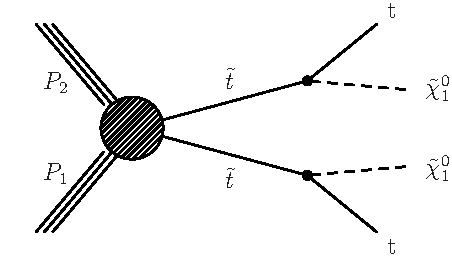
\includegraphics[width=0.40\textwidth]{figures/T2tt.pdf}
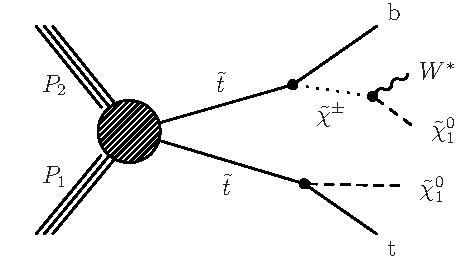
\includegraphics[width=0.40\textwidth]{figures/T2tb.pdf}\\
\caption{Signal models of interest in this search: 
top squark pair production with the top squark decaying into a top quark and 
neutralino or into a bottom quark and chargino.} 
\label{Fig:signal_diagrams}
\end{centering}
\end{figure}
%%%%%%%%%%%%%%%%%%%%%%%%%%%%%%%%%%%%%%%%%%%%%%%%%%

%%%%%%%%%%%%%%%%%%%%%%%%%%%%%%%%%%%%%%%%%%%%%%%%%%
\section{Detector and event reconstruction}
%%%%%%%%%%%%%%%%%%%%%%%%%%%%%%%%%%%%%%%%%%%%%%%%%%

%-------------
The CMS detector is a multi-purpose apparatus of cylindrical design with respect to the beams.  
%
The main features of the detector relevant to this analysis are described here; more details can be found in Ref.~\cite{CMS}.
%
A polar angle $\theta$ is defined with respect to the counterclockwise beam direction.  
%
A convenient coordinate is the pseudo-rapidity $\eta$, defined as $\eta = -\ln \tan (\theta/2)$.
%
Charged particle trajectories are measured by the silicon pixel and strip tracker, covering $|\eta| < 2.5$.
%
The tracker is immersed in a $3.8 \T$ magnetic field provided by a superconducting solenoid of $6{\rm m}$ in diameter that also encircles several calorimeters.
%
The tracker provides resolution of the transverse momentum, represented by \pt, of approximately 1.5\% for charged particles with $\pt\sim100$\GeVc.
%
A lead-tungstate crystal electromagnetic calorimeter (ECAL) and a brass-scintillator hadronic calorimeter (HCAL) surround the tracking volume and cover the region $|\eta| < 3$. 
%
Quartz-steel forward hadron calorimeters extend the coverage to $|\eta|\le 5$.
%
Muons are identified in gas ionization detectors embedded in the steel return yoke of the magnet.
%
The data for this analysis are recorded using a two level trigger system described in Ref.~\cite{CMS}.

%-------------
The recorded events are reconstructed using the particle-flow algorithm~\cite{PFT-09-001}. 
%
This algorithm reconstructs charged hadrons, neutral hadrons, photons, muons, and electrons using the information from the tracker, the ECAL and HCAL calorimeters, and the muon system.
%
The \METv is defined as the negative vector sum of the transverse momentum of all particles reconstructed in the event and \MET is the magnitude of the \METv vector.
%
All photons and neutral hadrons in an event, but only those charged particles which originate from the primary interaction, are clustered into jets using the anti-$k_\mathrm{T}$ clustering algorithm with the size parameter $0.4$~\cite{antikt}.
%
Neutral particles from overlapping pp interactions (``pileup"), and from the underlying events, are subtracted using the Fastjet technique~\cite{PU_JET_AREAS,JET_AREAS}, which is based on the calculation of the $\eta$-dependent transverse momentum density, evaluated on an event-by-event basis.
%
Jet energy-momenta are corrected using factors derived from simulation, and, for jets in data, an additional residual energy-momentum correction is applied to account for differences in the jet energy-momentum scales~\cite{JETJINST} between simulations and data.
%
Only jets with $\pt>30\GeVc$ are used in this search.

%-------------
For this analysis, a jet is considered a b-quark jet (b-tagged) if it passes  
the medium working point requirements of the "Combined Secondary Vertex" (CSV) method~\cite{bTagPAS}.
%
The b-quark identification efficiency is  67\% overall.
%
The probability of a jet originating from a light quark or gluon to be mis-identified as a b-quark jet is 1.4\%, averaged over \pt in \ttbar events~\cite{bTagPAS}.
%
For this analysis, b-tagged jets are required to have $\pt>30$\GeVc and be within $|\eta|<2.4$. 

%-------------
Muons are reconstructed using the muon detectors and by finding compatible track segments in the silicon tracker, and are required to be within $|\eta|<2.1.$
%
Electron candidates are reconstructed starting from a cluster of energy deposits in the ECAL that is then matched to the momentum associated with a track in the silicon tracker.
%
Electron candidates are required to have $|\eta|<1.44$ or $1.56<|\eta|<2.5$ to avoid the transition region between the ECAL barrel and the endcap.
%
Muon and electron candidates are required to originate within 2\,mm of the beam axis in the transverse plane.

%Jets are reconstructed with the Particle Flow (PF) technique and clustered with the anti-$k_\mathrm{T}$ algorithm with a resolution parameter D=0.4~\cite{antikt} (AK4).

%%%%%%%%%%%%%%%%%%%%%%%%%%%%%%%%%%%%%%%%%%%%%%%%%%
\section{Analysis Description}
%%%%%%%%%%%%%%%%%%%%%%%%%%%%%%%%%%%%%%%%%%%%%%%%%%

%-------------
The analysis is designed for maximum sensitivity to the T2tt model resulting in final states with many light-flavour jets, b-tagged jets, no leptons, and large \MET. 
%
Targeting the above-mentioned final states, data are initially selected by requiring a number of jets and b-jets (\njets and \nbjets) and a large \MET. 
%
The search regions are ultimately defined in exclusive bins of \ntops, \nbjets, \MET and a kinematic variable \MTTwo, defined in Sec.~\ref{sec:searchregions}. SM backgrounds come from processes such as QCD multijet events, Z bosons produced in association with jets (Z+jets), top quarks or W bosons produced in association with jets (t/W+jets), and smaller contributions from rare SM processes.
%
%The top reconstruction and identification procedure (top tagging) is described in this section, as well as the Monte Carlo (MC) samples that model signal and backgrounds.
%
%The data selection process starts with the trigger requirements and follows with a pre-selection and the definition of the search bins. 

%%%%%%%%%%%%%%%%%%%%%%%%%%%%%%%%%%%%%%%%%%%%%%%%%%
\subsection{Top quark reconstruction and identification}
%%%%%%%%%%%%%%%%%%%%%%%%%%%%%%%%%%%%%%%%%%%%%%%%%%

%-------------
The procedure to reconstruct and identify the hadronically-decaying top quarks (top-tagging) in the 2015 13~TeV analysis is similar to the one used in Ref.~\cite{stop8TeV}, where reconstruction of the hadronically decaying top quarks is performed as described in Refs.~\cite{Kaplan:2008ie,Plehn:2010st,Kaplan:2012gd}.  
%
The collection of four or more jets from events in the pre-selection sample is divided into all possible sets of three jets and a remnant system, where the remnant system must contain at least one b-tagged jet. 
%
The fully reconstructed top quark is one of the three-jet (trijet) combinations. 
%
To be considered as a fully reconstructed top quark, the trijet system must satisfy the following requirements. 
%
(i) Each jet lies within a cone of radius 1.5 in ($\eta,\phi$) space, centered at the direction defined by the trijet combination. 
%
The radius requirement implies a moderate Lorentz boost of the top quark as expected for events with large $\Delta m = m_{\sTop} - m_{\chiOneZero}$ targeted in this search.
%
(ii) The trijet system mass ($m_{\text{3-jet}}$) must be within the range 100-250~\GeVcc.
%
(iii) The trijet system must satisfy one of the three following criteria:
\begin{equation} \label{eq:taggerEQ}
   \begin{array}{l}
     \displaystyle{
     \mbox{a)}~~ 0.2< \arctan\left(\frac{m_{13}}{m_{12}}\right) < 1.3 ~~\mbox{and}~~ R_\mathrm{min} < \frac{m_{23}}{m_{\text{3-jet}}} < R_\mathrm{max}}, \\
     %%
     \displaystyle{
     \mbox{b)}~~ R_\mathrm{min}^{2}\left(1+\left(\frac{m_{13}}{m_{12}}\right)^2\right) 
     < 1-\left(\frac{m_{23}}{m_{\text{3-jet}}}\right)^2 
     < R_\mathrm{max}^{2}\left(1+\left(\frac{m_{13}}{m_{12}}\right)^2\right) ~~\mbox{and}~~ \frac{m_{23}}{m_{\text{3-jet}}} > 0.35}, \\
     %%
     \displaystyle{
     \mbox{c)}~~ R_\mathrm{min}^{2}\left(1+\left(\frac{m_{12}}{m_{13}}\right)^2\right) 
     < 1-\left(\frac{m_{23}}{m_{\text{3-jet}}}\right)^2 
     < R_\mathrm{max}^{2}\left(1+\left(\frac{m_{12}}{m_{13}}\right)^2\right) ~~\mbox{and}~~ \frac{m_{23}}{m_{\text{3-jet}}} > 0.35}. \\
   \end{array} 
\end{equation}
%
Here, $m_{12}$, $m_{13}$, and $m_{23}$ are the dijet masses, where the jet indices 1, 2, and 3 are \pt ordered.
%
The following numerical constants have values $R_\mathrm{min} = 0.85\cdot(m_{\W}/m_{\mathrm{\topquark}})$, $R_\mathrm{max} = 1.25\cdot(m_{\W}/m_{\mathrm{\topquark}})$, $m_{\W} = 80.4$~\GeV, and $m_{\mathrm{\topquark}} = 173.4$~\GeV~\cite{PDG}.
%
The top-quark tagging (t-tagging) conditions of a), b), or c) can be reduced (under certain approximations detailed in Ref.~\cite{Plehn:2010st}) to the requirement that $m_{23}/m_{\text{3-jet}}$, $m_{12}/m_{\text{3-jet}}$, or $m_{13}/m_{\text{3-jet}}$, respectively, be consistent with the $m_{\W}/m_{\mathrm{\topquark}}$ ratio.
%
The other conditions are motivated by the Lorentz structure of the tW coupling and suppress contributions from light-quark and gluon jets~\cite{Plehn:2010st}. 
%
If multiple trijet combinations satisfy these criteria, the triplet with mass closest to the top quark mass is selected.

%-------------
The top-tagging algorithm is improved in this work, compared with ~\cite{stop8TeV}, to be sensitive to boosted senarios where decay products from the $W$ boson or top quark are merged.  
%
Specifically, the jet mass is used to determine if the jet represents the merged decay products of a $W$ boson (merged $W$ jet) or a top quark (merged top jet).  
%
When the jet mass is in the 70-110 \gev range, it is considered as a $W$ boson, and a top quark when it is in the 110-220 \gev range.
%
Once a merged $W$ boson jet is identified, an additional jet is combined with it to form a potential top candidiate. 
%
The merged $W$ boson jet is treated as a ``dijet'' system in the top tagging algorithm, and  $R_{min} < m_W/m_{W+j} < R_{max}$ is used as a criteria to decide if it is a good top candidate. 
%
In case a single jet is identified as a top quark jet, it is simply treated as a top candidate. 
%
For merged top quark jets, the tagger has good efficiency over a wide range of top quark \pt, from $\sim25\%$ at 200 \gev to close to 80\% at 1~TeV. 

%%%%%%%%%%%%%%%%%%%%%%%%%%%%%%%%%%%%%%%%%%%%%%%%%%
\subsection{Trigger path}
\label{sec:trig}
%%%%%%%%%%%%%%%%%%%%%%%%%%%%%%%%%%%%%%%%%%%%%%%%%%

%-------------
Events in the search regions, as well as the single-lepton and multijet samples for electroweak and QCD background estimations are collected from a Level 1 hardware trigger which applies a threshold on the scalar summed transverse energy over all (calorimeter-only) jets in the event of at least 175~\GeV. 
%
If the event is accepted, the high-level trigger then requires a calorimeter-based \HT $>280$ \gev and a calorimeter-based \met $>70$ \gev.  
%
Finally, the high-level trigger applies a threshold on the scalar summed transverse momenta (\HT) over all particle flow based jets in the event of greater than 350~\GeV in coincidence with a threshold on the missing transverse momentum (\MET) above 100~\GeV computed using all particle flow candidates in the event.  
%
Studies show that this analysis is fully efficient, if one requires at least 175~\GeV of particle-flow based \MET together with at least 500~\GeV of particle-flow based $H_{\rm T}$.

%%%%%%%%%%%%%%%%%%%%%%%%%%%%%%%%%%%%%%%%%%%%%%%%%%
\subsection{Pre-selection}
\label{sec:pre-selection}
%%%%%%%%%%%%%%%%%%%%%%%%%%%%%%%%%%%%%%%%%%%%%%%%%%

%-------------
The search looks for multijet events, with b-jets decaying from top quarks, large \MET and no leptons. 
%
Initially, a loose pre-selection selection is applied in \MET, \njets and \nbjets, which preserves 2-20\% of the signal events. 
%
The events passing the pre-selection selection are then later classified into search regions. 
%
The following criteria define the pre-selection selection.

%-------------
All events must pass filters designed to remove detector- and beam-related noise.  
%
All jets considered in this analysis are required to have $\pt>$30 \gev and $|\eta|<$2.4.  
%
In addition, all jets must pass a set of ``loose'' jet identification criteria. 
%
The minimum number of such jets in an event must be $\njets\geq4$, with the leading two jets required to have $\pt>$50 \gev.  
%
The missing transverse momentum must satisfy \MET $\ge$ 200 \gev, where the threshold is chosen so as to be well on the trigger efficiency plateau and also to allow a low 175~\GeV $\<$ \MET sideband for background studies.  
%
The scalar summed transverse momentum of the event must satisfy \HT $\ge$ 500 \gev, with \HT = $\sum_{\mathrm{jets}} \pt$, also chosen to be on the trigger efficiency plateau.  
%
Jets in the \HT calculation must meet the same jet seletion criteria defined above.  
%
The number of heavy-flavor tagged jets in the event must satisfy \nbjets $\ge$ 1, with b-jets identified using the CSV b-tagging algorithm (CSVM), medium working point.
%
Events are vetoed if they contain isolated muon candidates that satisfy $\pt>$10 \gev and $|\eta|<$2.4.
%
A relative-isolation criteria is enforced for which an isolation cone shrinks as a function of increasing muon \pt. 
%
The \pt in the shrinking cone is required to be less than 20\% of the muon \pt. 
%
Events are further vetoed if the contain isolated electron candidates that have $\pt>$10 \gev and $|\eta|<$2.5. 
%
Isolated electrons are determined using a similar isolation requirement as for muons, except that less than 10\% of the electron energy is required to be in the shrinking isolation cone.
%
A requirement on the angle between \MET and the first three leading jets, $\Delta\phi(\MET, j_{1,2,3})>$ 0.5, 0.5, 0.3, is applied to remove events coming from QCD processes.
%
After applying the cuts described above the residual background comes from \ttbar, single top, and $W+$jets events with one $W\rightarrow l\nu$ decay where $l$ can be an electron, muon or tau decaying hadronically. 
%
To further suppress these backgrounds, we reject events that have one or more isolated tracks. 
%
The track isolation is calculated from charged PF candidates consistent with the reconstructed primary vertex ($|dz(PV)|<0.1~\mathrm{cm}$).
%
The requirements are different for muon, electron and charged hadron tracks.
%
For both electron and muon tracks, the isolated track requirements are: $\pt>$5 \gev, $|\eta|<$2.5 and a relative isolation of less than 0.2.
%
For charged hadron tracks, the \pt requirement is raised to be at least 10 \gev and the relative isolation value to be less than 0.1. 
%
To improve signal-to-background event discrimination, events with one isolated track, as defined above, are only rejected if they satisfy $m_T(tk,\met) = \sqrt{2p_{T}^{tk}\met(1-\cos\Delta\phi)}<100\;\mathrm{GeV}$, where $p_{T}^{tk}$ is the transverse momentum of the track and $\Delta\phi$ is the azimuthal separation between the track and \METv. 
%
Tables~\ref{tab:cutflowMC1},~\ref{tab:cutflowMC2} in Appendix~\ref{sec:appendixcutflow} illustrate the effect of the pre-selection cuts on background SM processes using MC simulation. Table~\ref{tab:cutflowMC3} in Appendix~\ref{sec:appendixcutflow} shows the effects of the pre-selection cuts on two example signal models.  

%%%%%%%%%%%%%%%%%%%%%%%%%%%%%%%%%%%%%%%%%%%%%%%%%%
\subsection{Search region selections}
\label{sec:searchregions}
%%%%%%%%%%%%%%%%%%%%%%%%%%%%%%%%%%%%%%%%%%%%%%%%%%

%-------------
We bin the search regions in terms of the number of b-tagged jets and top candidates. 
%
A top candidate is defined to be an object that satifies the top-tag criteria as shown in equation~\ref{eq:taggerEQ} with the QCD rejection cut removed ($m_{23}/m_{3-jet}>$0.35). 
%
If a top candidate is reconstructed in the event and a b-tagged jet identified in the remaining system (R-sys), this candidate is added first to the top counting list. 
%
Events with only one top candidate and no b-tagged jet in the R-sys are rejected.
%
Additional top candidates reconstructed from the R-sys are considered, starting from those with mass closest to the top quark mass. 
%
To avoid any two top candidates to share the same jets, we verify that the additional top candidate does not include a jet identified as part of an existing candidate. 
%
If it does, the additional candidate is discarded. 
%
Note that, as stated in Ref.~\cite{stop8TeV}, the top candidate definition has no explicit requirement on b-tagged jets. 
%
Thus there is not a one-to-one correspondence between the number of top candidates and the number of b-tagged jets in an event.  
%
The number of b-jets and top candidates variables are binned as $\nbjets=1$, $\nbjets=2$ and $\ntops=1$, $\ntops=2$. 
%
Exclusive search regions are defined for all combinations of \nbjets and \ntops bins.
%

%-------------
To improve background suppression, in particular the \ttbar contribution, the \MET and \MTTwo variables are added to the set that defines the search regions. 
%
The variable \MTTwo~\cite{Lester:1999tx,Barr:2003rg} is an extension of the transverse mass variable that is sensitive to the pair production of heavy particles, each of which decays to an invisible particle.
%
The \pTop, the \pRsystem, and the \MET in an event are used to constructed \MTTwo assuming the invisible particles are massless.
%
The \MTTwo variable is defined as:
%%%%%%%%%%%%%%%%%%%%%%%%%%%%%%%%%%%%%%%%%%%%%%%%%%
\begin{equation} \label{eq:MT2}
   \begin{array}{l}
     \displaystyle{ \MTTwo \equiv \min_{\vec{q}_{T}^{(1)}+\vec{q}_{T}^{(2)} = \vec{p}_{T}} [\max\{m_{T}^2(\vec{p}_{T}^{t^{(1)}}, \vec{q}_{T}^{(1)}; m_{\chi_1^0}), m_{T}^2(\vec{p}_{T}^{t^{(2)}}, \vec{q}_{T}^{(2)}; m_{\chi_1^0})\}]  } 
   \end{array}
\end{equation}
%%%%%%%%%%%%%%%%%%%%%%%%%%%%%%%%%%%%%%%%%%%%%%%%%%
where the $m_{T}^2$ is the transverse mass,
%%%%%%%%%%%%%%%%%%%%%%%%%%%%%%%%%%%%%%%%%%%%%%%%%%
\begin{equation} \label{eq:MTdef}
   \begin{array}{l}
     \displaystyle{
        m_{T}^2(\vec{p}_{T}^{t^{(1)}}, \vec{q}_{T}^{(1)}; m_{\chi_1^0}) \equiv m_{t^{(1)}}^{2} + m_{\chi_1^0}^2 + 2(E_{T}^{t^{(1)}}E_{T}^{(1)} - \vec{p}_{T}^{t^{(1)}} \cdot \vec{q}_{T}^{(1)})
     }
   \end{array}
\end{equation} 
%%%%%%%%%%%%%%%%%%%%%%%%%%%%%%%%%%%%%%%%%%%%%%%%%%
\MTTwo is a minimization of two transverse masses with a constraint that the sum of the transverse momenta of both $\chi_1^0$'s is equal to the missing transverse momentum of the event, i.e., $\vec{q}_{T}^{(1)}+\vec{q}_{T}^{(2)} = \vec{p}_{T}$. 
%
\MTTwo has a kinematic upper limit which is the \sTop mass. 
%
The superscripts $(1)$ and $(2)$ in the equations refer to the individual decays of the \sTop particles. 
%
In the specific case of the analysis described in this summary, we replace the quantities related to superscript $(1)$ by those of associated with the fully reconstructed top quark, i.e., the \pTop. 
%
Similarly, we replace the quantities related to superscript $(2)$ by those of the partially reconstructed top quark, i.e., the \pRsystem  for $\ntops =1$ and the fully reconstructed top quark for $\ntops \ge 2$. \MET then corresponds to $\vec{p}_{T}$ in the equation~\ref{eq:MT2}. 
%
Since we assume that the invisible particle is massless, $m_{\chi_1^0}$ should be zero in Eqs.~\ref{eq:MT2}-~\ref{eq:MTdef}. 

%-------------
We start from the fact that, by construction, there is always at least one hadronic top candidate in events that lie in the search bins. 
%
If there are two top candidates, \MTTwo is calculated using the pair of top candidates and \met. 
%
In the case of more than two top candidates, we compute \MTTwo for all combinations and choose the \MTTwo with the smallest value. 
%
If only one top candidate is identified by the top-tagging algorithm, we reconstruct the other top quark from the remanent of the event using the b-tagged jet as a seed and the R-sys jet closest to the b-tagged jet with an invariant mass between 50 \gev and the top quark mass. 
%
In case no R-sys jet combination satisfies that invariant mass requirement, we use the b-tagged jet as the only remanent of the other top quark. 
%
In the latter case, \MTTwo is calculated from the reconstructed top candidate, the remanent and the \met.

%-------------
Figure~\ref{fig:compSBvars} demonstrates the background composition following the pre-selection cuts and as a function of \ntops, \nbjets, \MET and \MTTwo, which are used to define the search bins.
%%%%%%%%%%%%%%%%%%%%%%%%%%%%%%%%%%%%%%%%%%%%%%%%%%
\begin{figure}[h]
  \begin{center}
    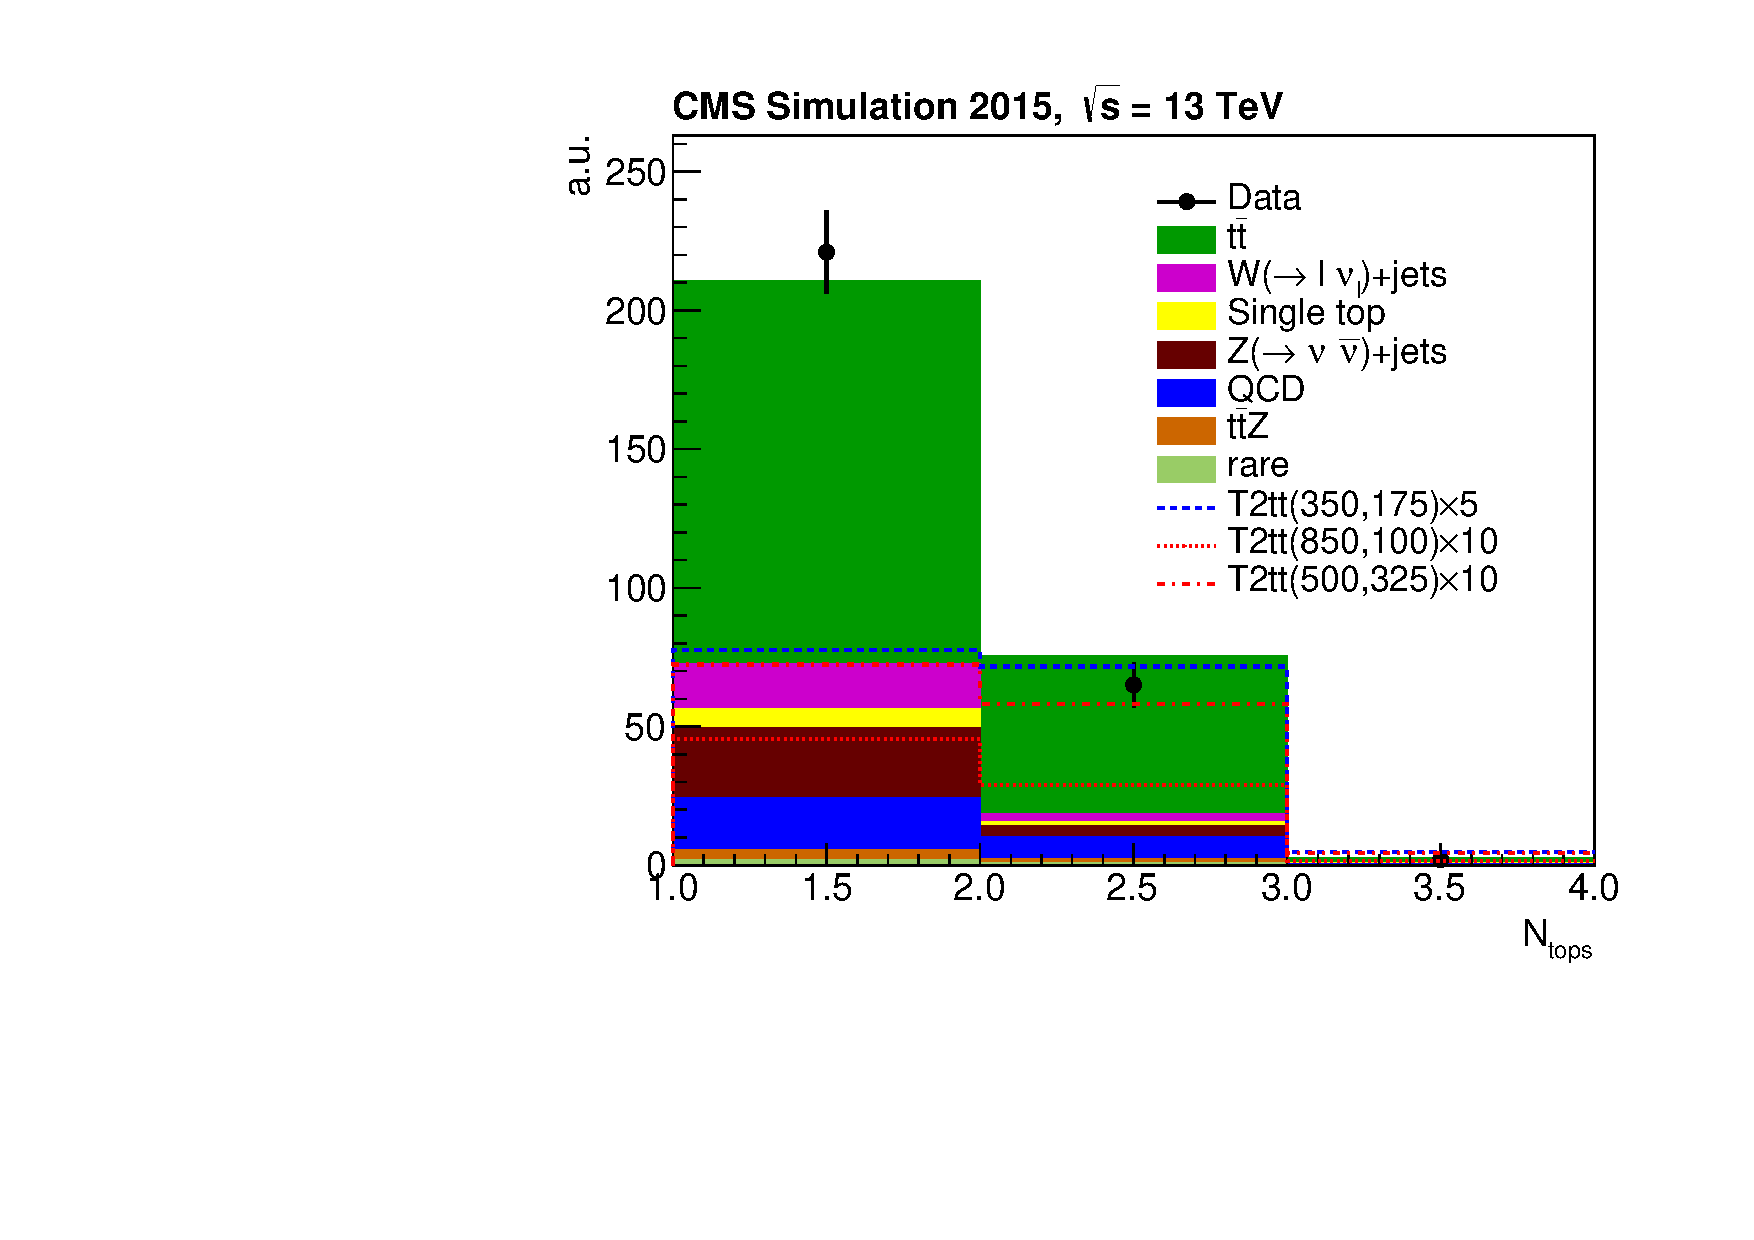
\includegraphics[width=0.48\linewidth]{figures/comb_nTops_baseline.pdf}
    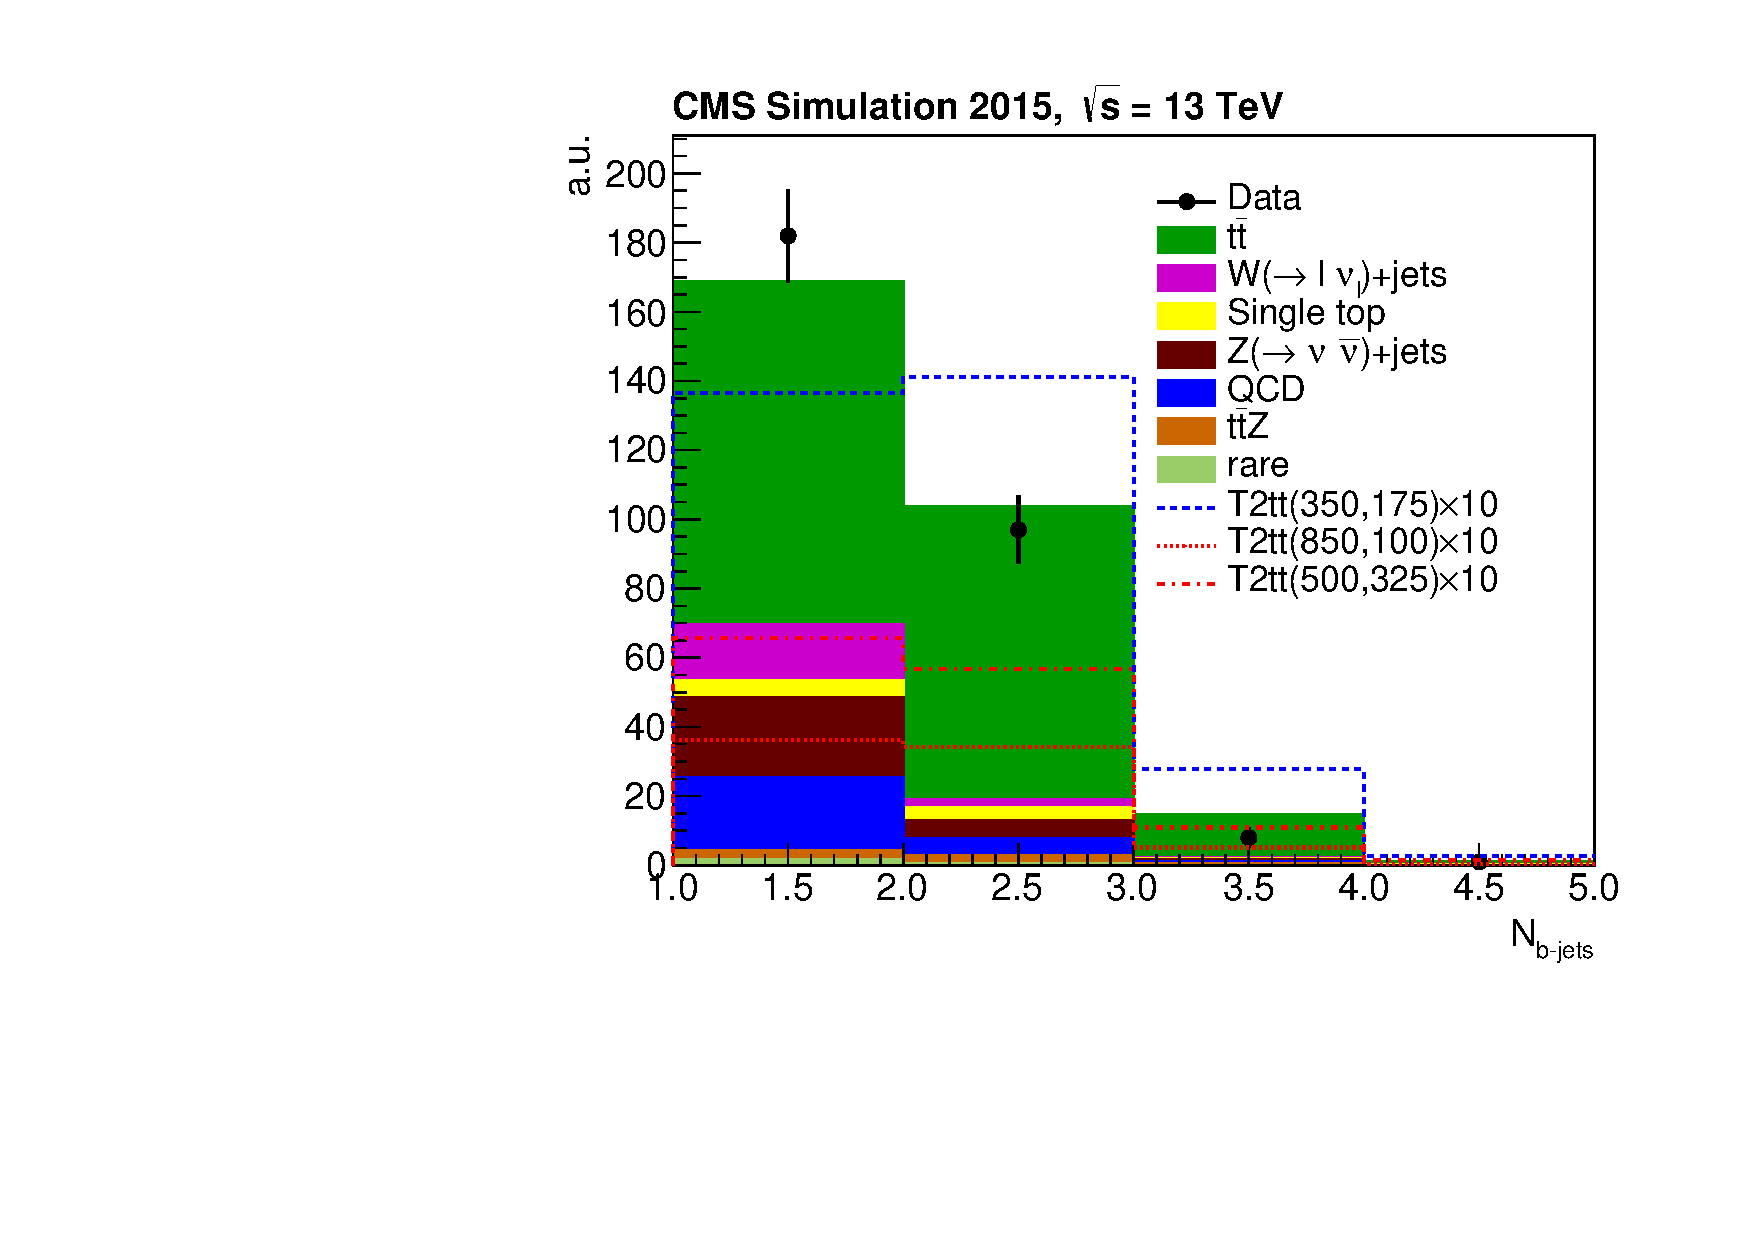
\includegraphics[width=0.48\linewidth]{figures/comb_nbJets_baseline.pdf} \\
    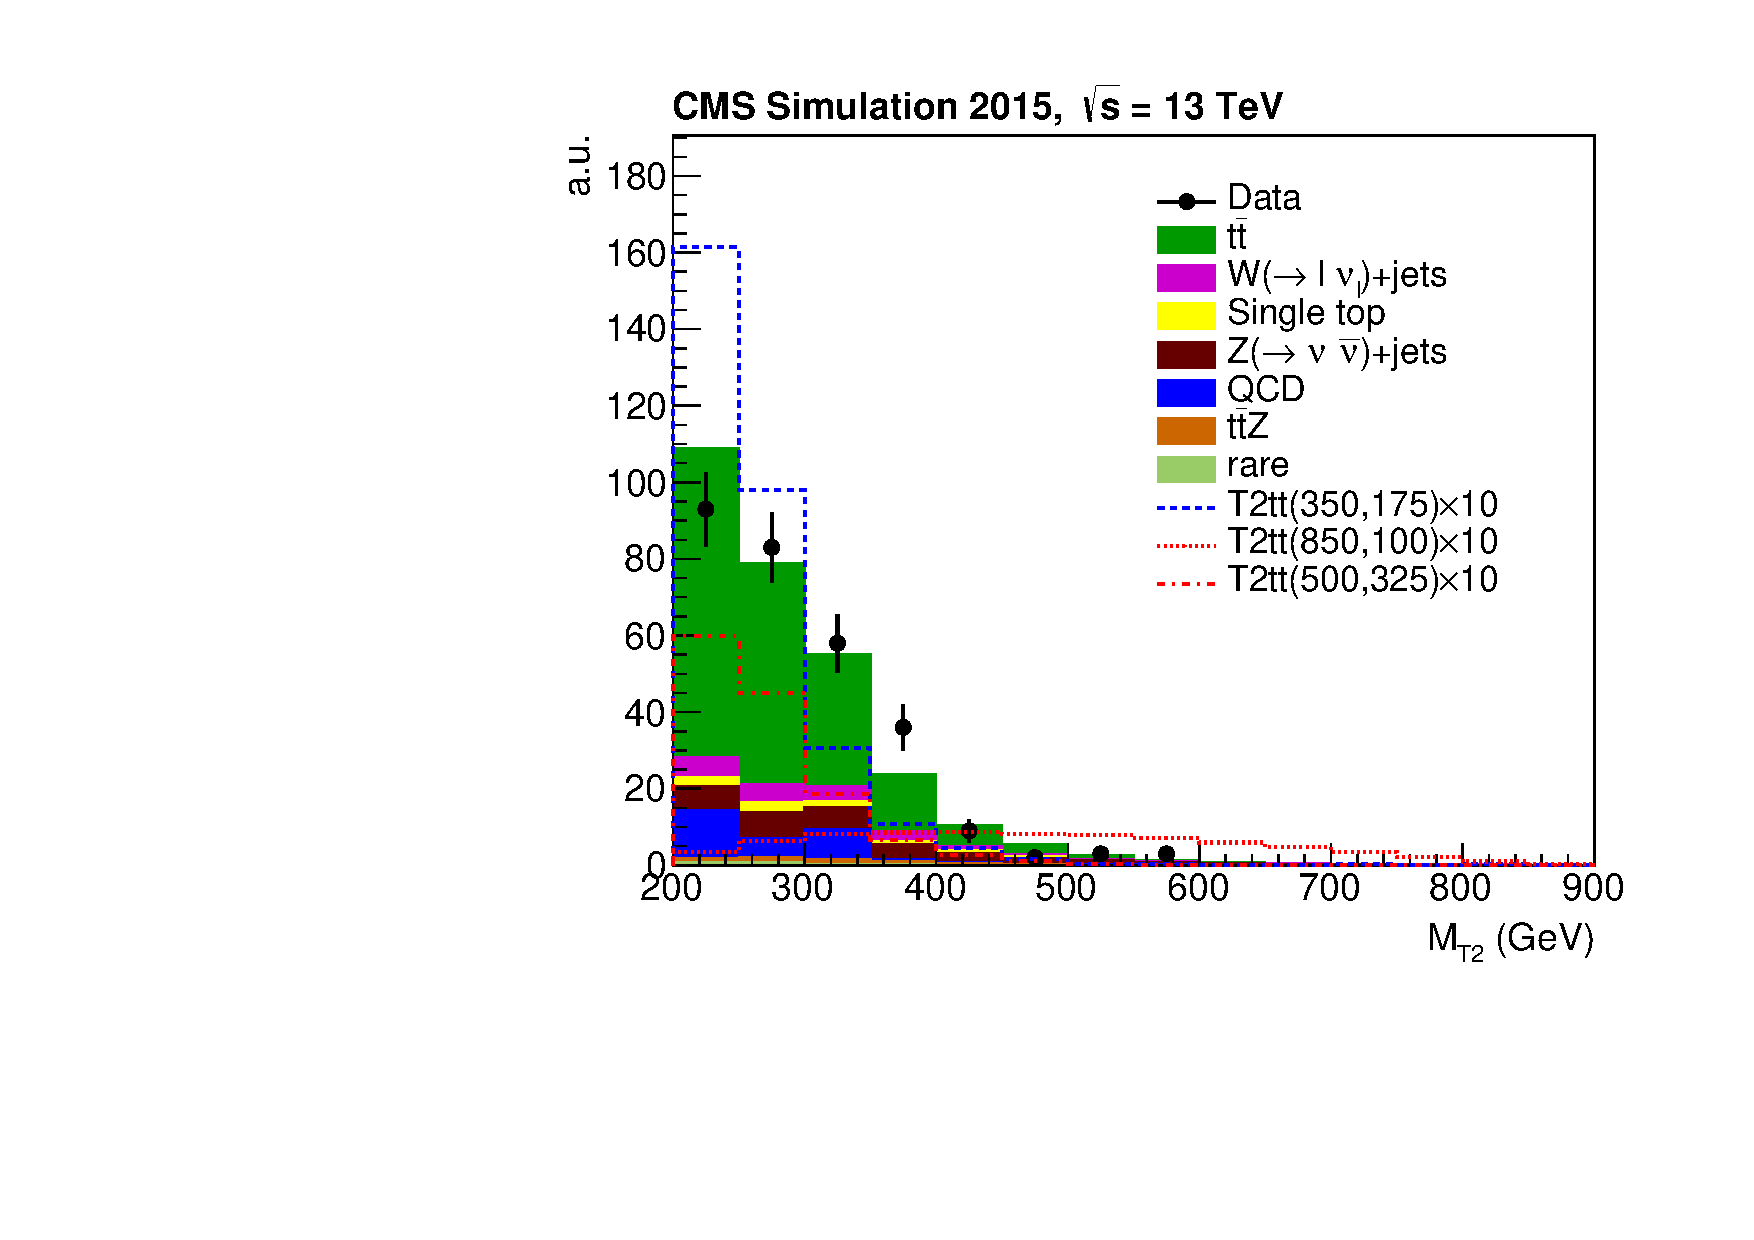
\includegraphics[width=0.48\linewidth]{figures/comb_MT2_baseline.pdf}
    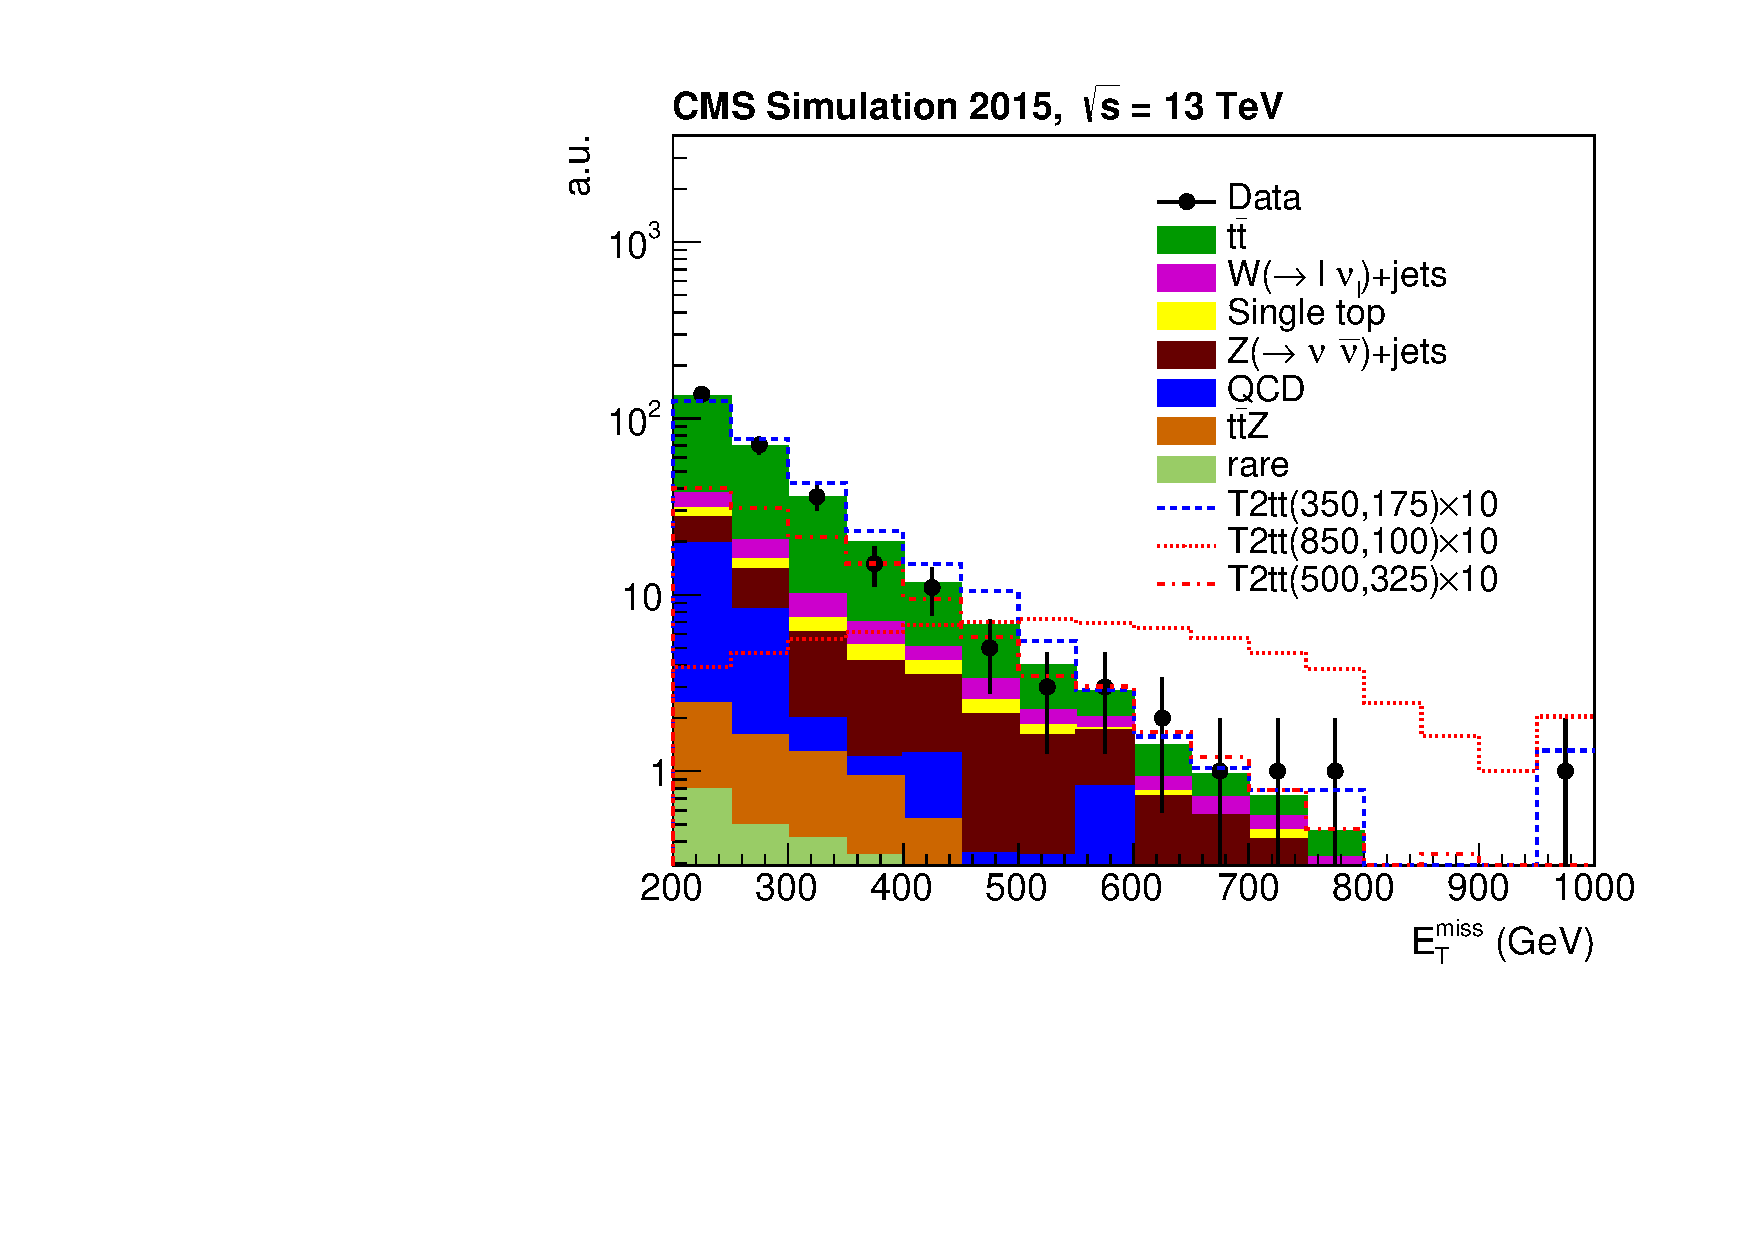
\includegraphics[width=0.48\linewidth]{figures/comb_met_baseline.pdf}
    \caption{ Comparison of the distributions between total SM backgrounds from simulation and several signal points for \ntops, \nbjets, \MET and \MTTwo clock-wise. }
    \label{fig:compSBvars}
  \end{center}
\end{figure}
%%%%%%%%%%%%%%%%%%%%%%%%%%%%%%%%%%%%%%%%%%%%%%%%%%
The search bins defined after pre-selection cuts are illustrated in Fig.~\ref{fig:SBXX}. 
%%%%%%%%%%%%%%%%%%%%%%%%%%%%%%%%%%%%%%%%%%%%%%%%%%
\begin{figure}[h]
  \begin{center}
    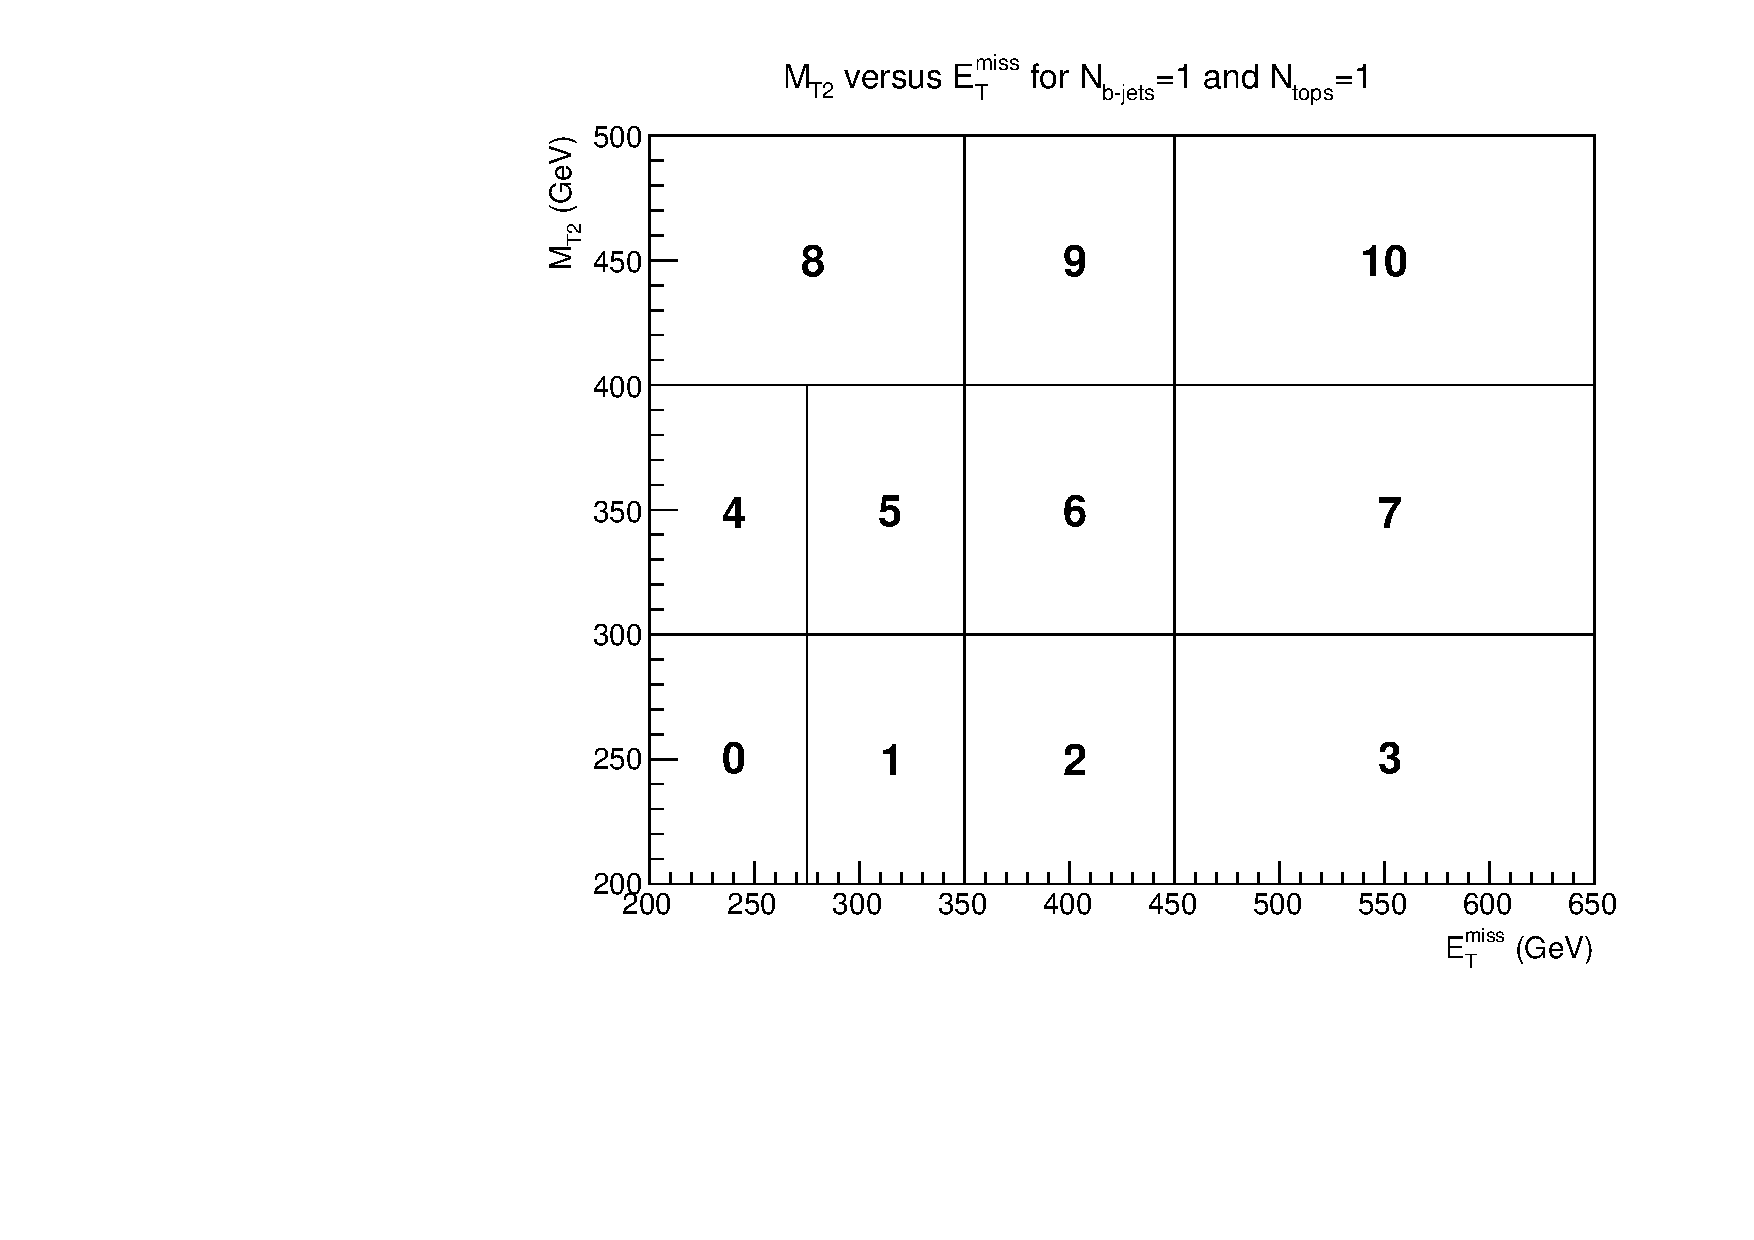
\includegraphics[width=0.45\linewidth]{figures/poly_MT2_vs_met_merged_0.pdf}
    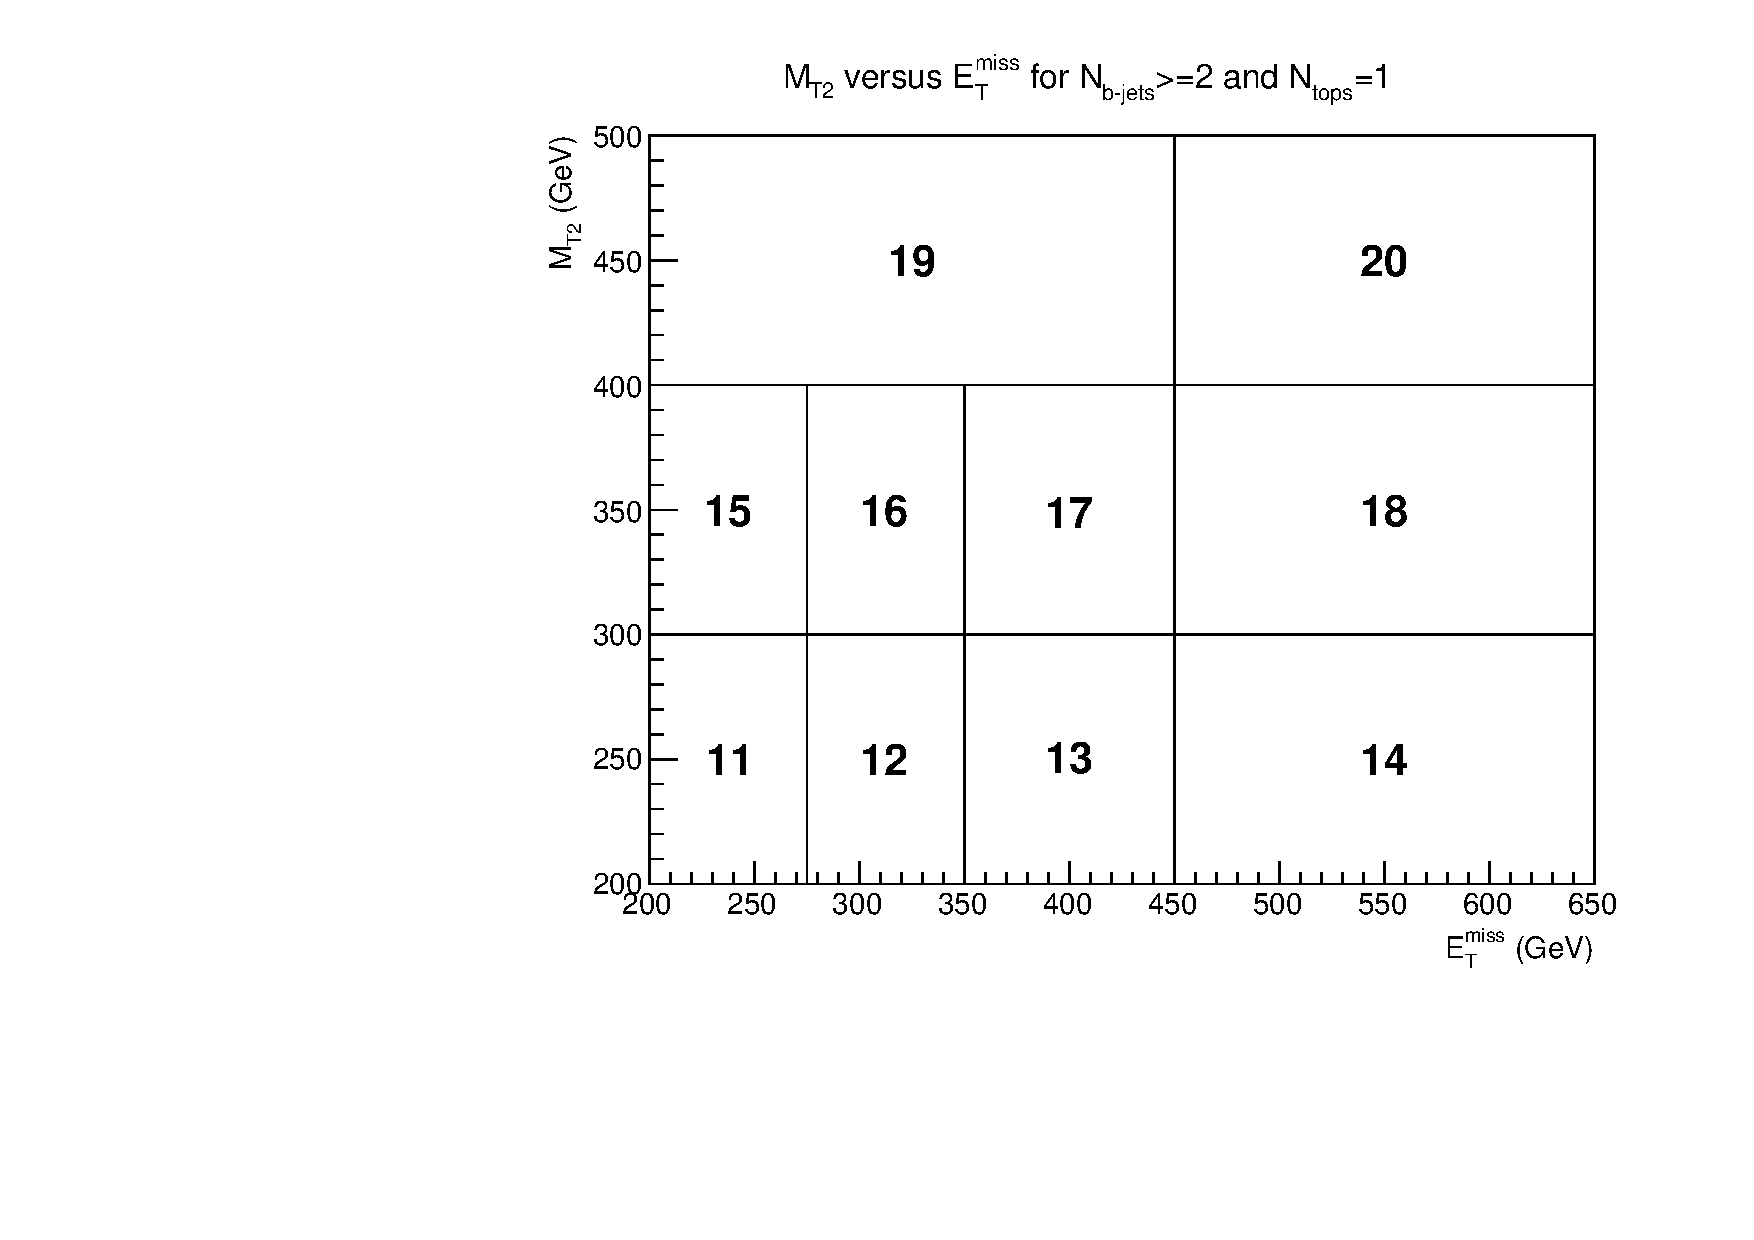
\includegraphics[width=0.45\linewidth]{figures/poly_MT2_vs_met_merged_1.pdf} \\
    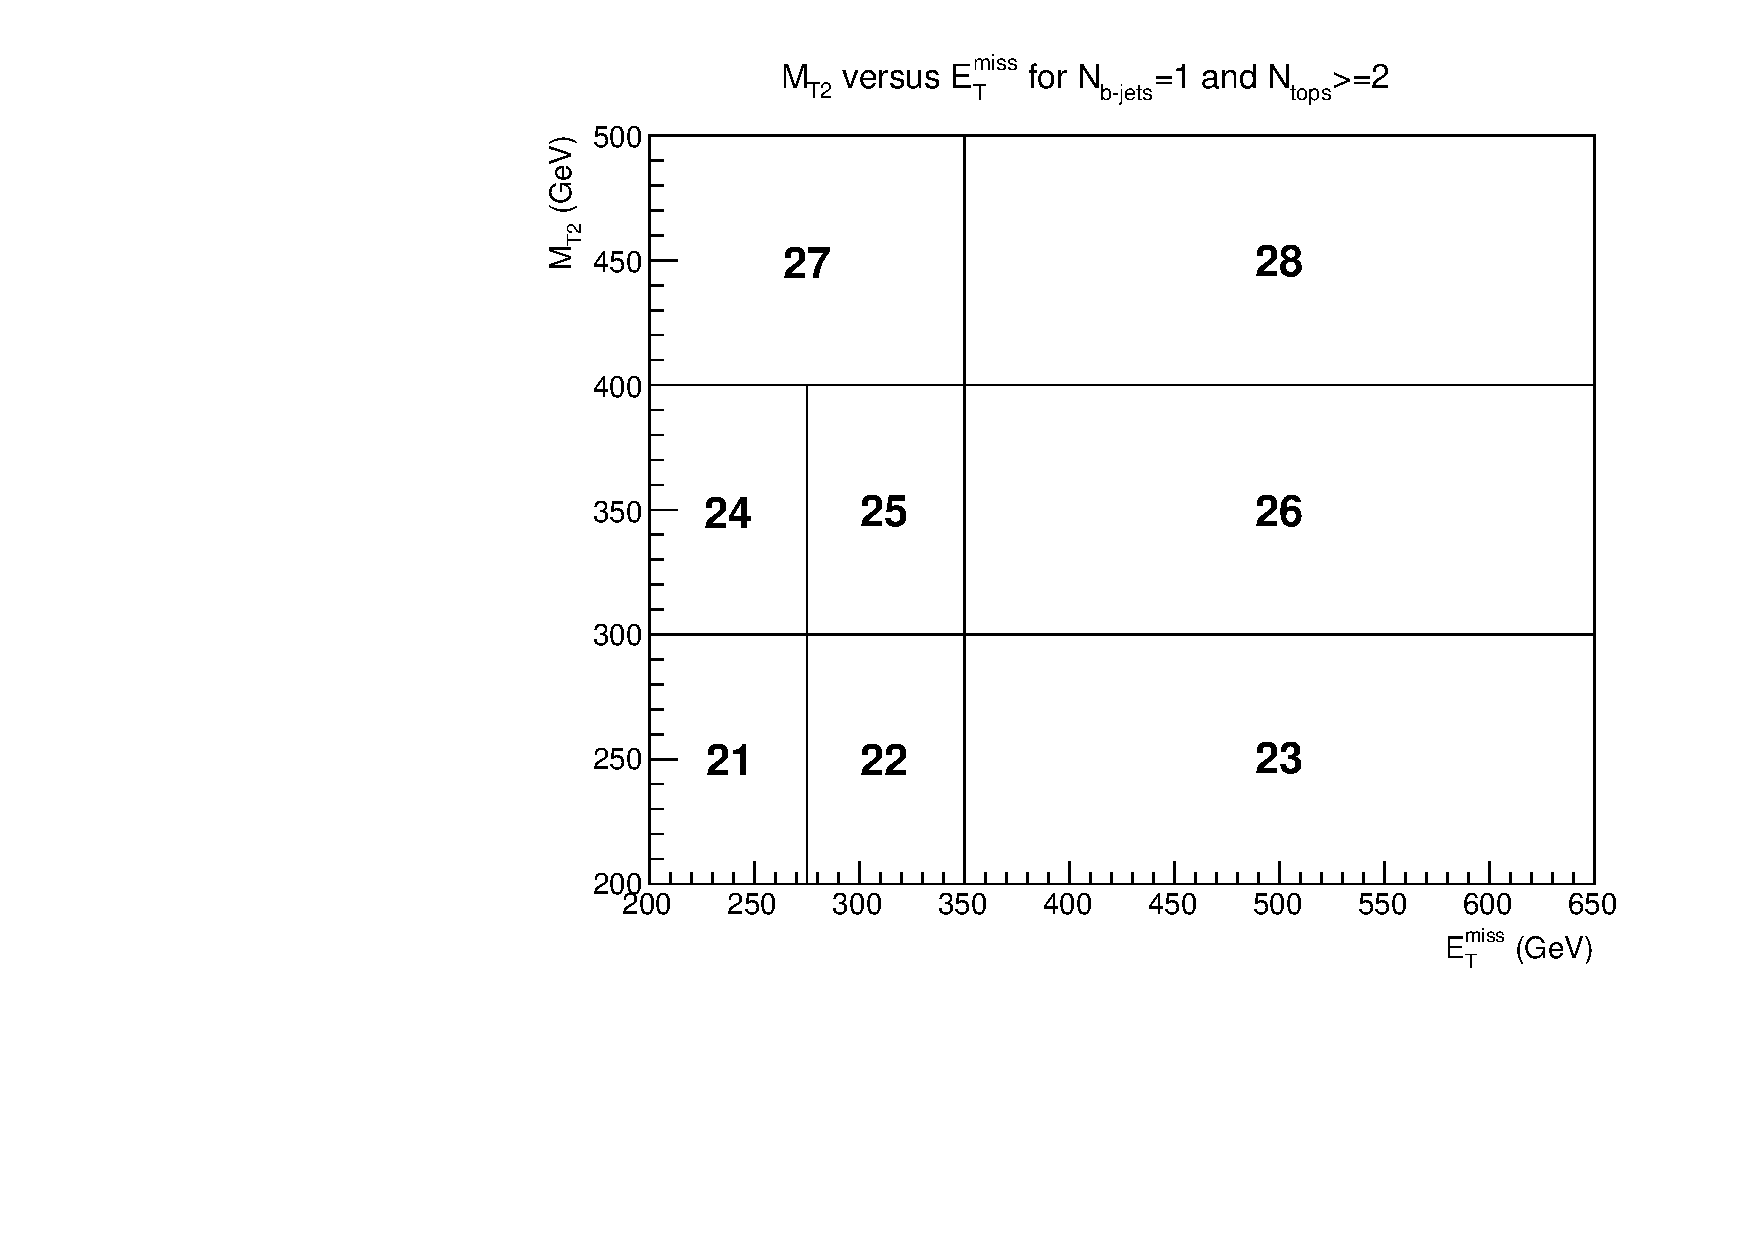
\includegraphics[width=0.45\linewidth]{figures/poly_MT2_vs_met_merged_3.pdf} 
    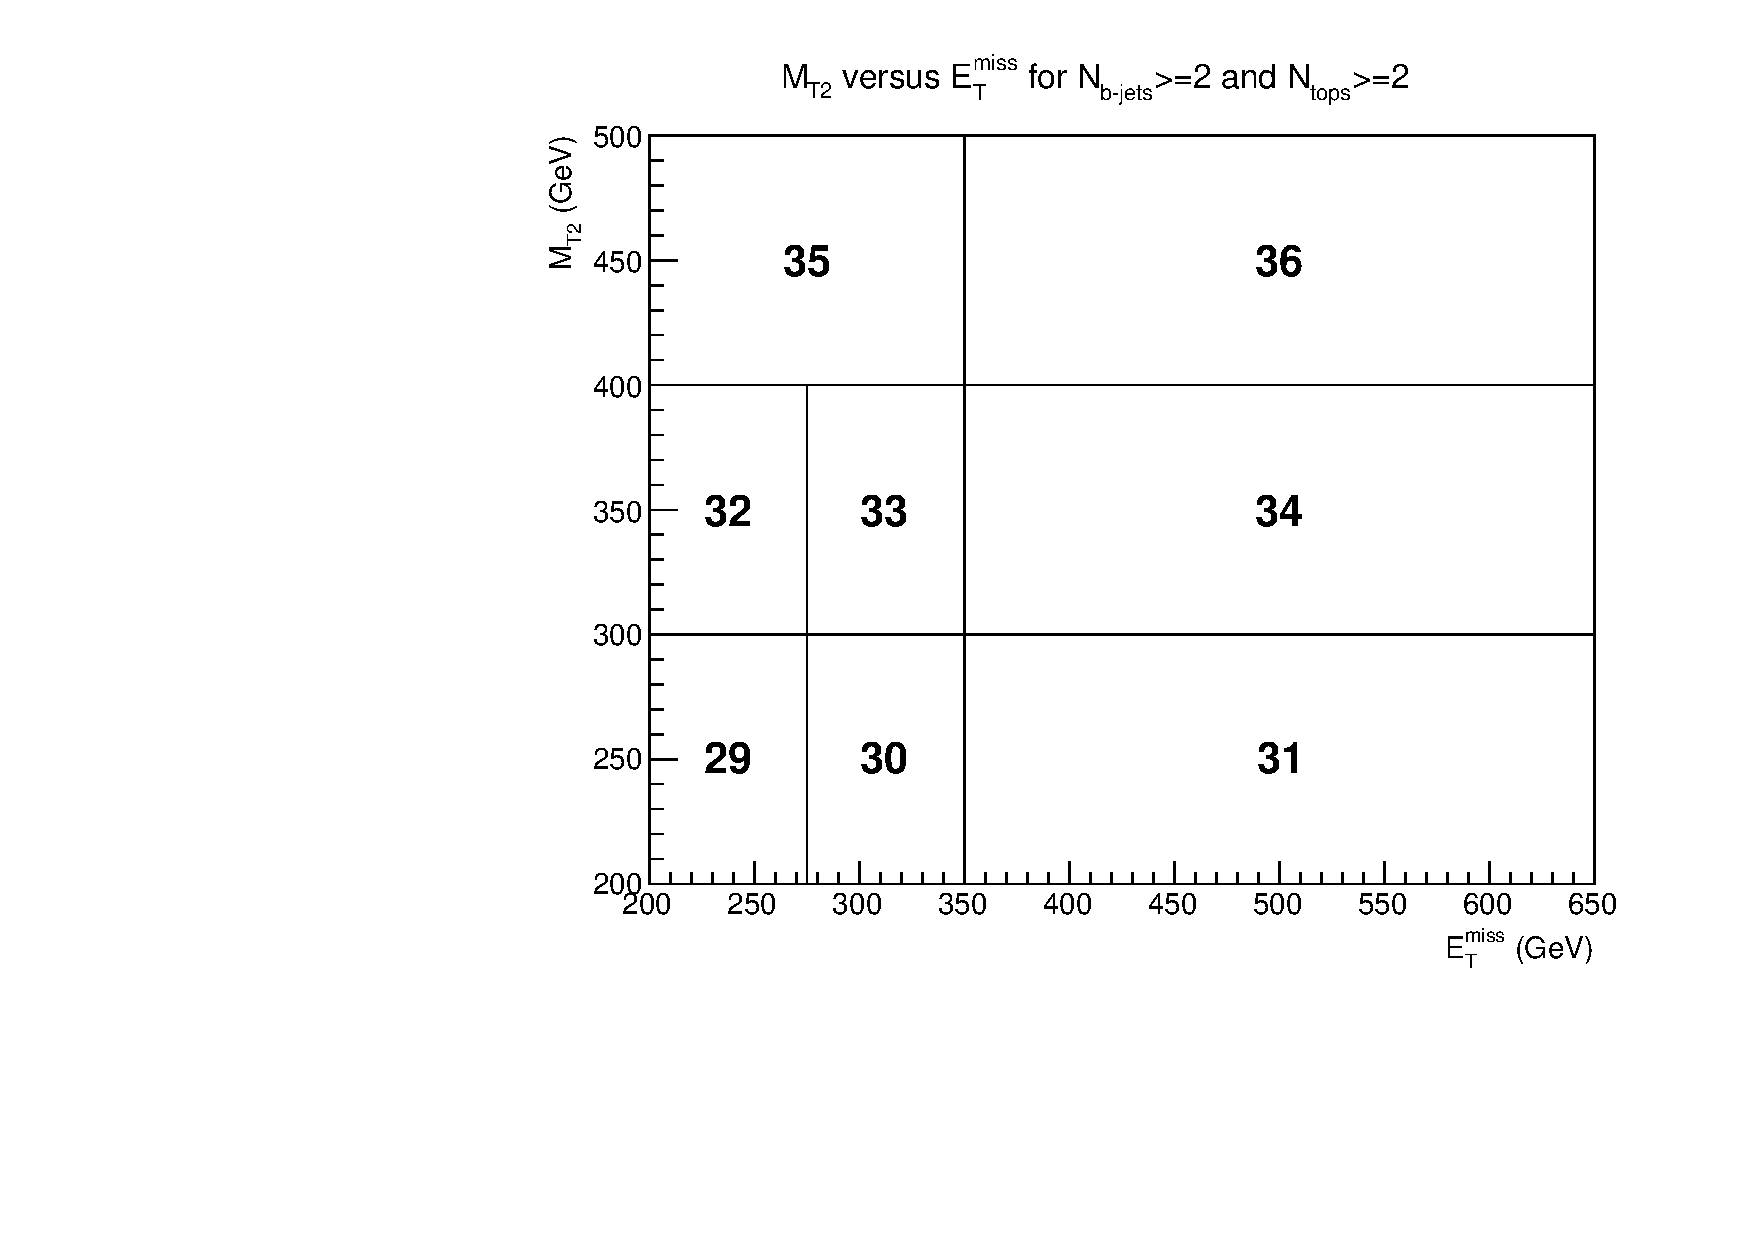
\includegraphics[width=0.45\linewidth]{figures/poly_MT2_vs_met_merged_4.pdf} \\
    \caption{ Search bin definitions after pre-selection cuts. }
    \label{fig:SBXX}
  \end{center}
\end{figure}
%%%%%%%%%%%%%%%%%%%%%%%%%%%%%%%%%%%%%%%%%%%%%%%%%%
The numbers displayed in the figures are the binning indices which are used throughout the analysis.


%%%%%%%%%%%%%%%%%%%%%%%%%%%%%%%%%%%%%%%%%%%%%%%%%%
\subsection{Monte Carlo simulated event samples}
%%%%%%%%%%%%%%%%%%%%%%%%%%%%%%%%%%%%%%%%%%%%%%%%%%

%-------------
The analysis uses a set of Monte Carlo (MC) samples for background estimation method development and predictions as well as SUSY signal samples for interpretation of the results in the light of a number of simplified models. The {\MADGRAPH}5~\cite{Alwall:2011uj} event generator is used to simulate \ttbar, \wjets, \zjets, and QCD multijet events.
%
Single-top events in the $t$ and $\cPqt\PW$ channels are described using the \POWHEG v1.0~\cite{Nason:2004rx,Frixione:2007vw,Alioli:2010xd,Alioli:2009je,Re:2010bp} program, and in the $s$ channel using the {\MADGRAPH}5{\textunderscore}a{\MCATNLO}~\cite{Alwall:2014hca} program. 
%
The latter generator is also used to simulate events with dibosons ($\PW\PW$, $\cPZ\cPZ$, and $\PW\PH$ production, etc., with $\PH$ a Higgs boson) and rare processes ($\ttbar\PW$, $\ttbar\cPZ$, and $\PW\PW\cPZ$ combinations, etc.), except that \POWHEG~\cite{Melia:2011tj} is used for $\PW\PW$ events in which both {\PW} bosons decay leptonically.
%
Simulation of the detector response is based on the \GEANTfour~\cite{Agostinelli:2002hh} package. 
%
All cross sections come from calculations performed at next-to-next-to-leading-order (NNLO), unless otherwise noted.  
%
All simulated samples include pile-up with an average of 20 interactions per bunch crossing and a 25~ns interval between bunches.
%-------------
Signal T2tt and T2tb events are simulated for a range of stop \mstop LSP \mlsp mass values, with $\mlsp<\mstop$.
%
The signal samples are based on the \MADGRAPH generator, with up to two partons present in addition to the stop pair. 
%
The decays of the stop are described with a pure phase-space matrix element~\cite{Sjostrand:2014zea}. 
%
The signal production cross sections are computed~\cite{bib-nlo-nll-01,bib-nlo-nll-02,bib-nlo-nll-03,bib-nlo-nll-04,bib-nlo-nll-05} with next-to-leading order (NLO) plus next-to-leading-logarithm (NLL) accuracy. 
%
To reduce computational requirements, the detector is modeled with the CMS fast simulation program~\cite{Orbaker:2010zz,bib-cms-fastsim-02}, which yields consistent results compared with the {\GEANTfour}-based simulation.
%-------------
The NNPDF3.0LO~\cite{Ball:2014uwa} parton distribution functions (PDF) are used for the \MADGRAPH signal and background samples, and the NNPDF3.0NLO~\cite{Ball:2014uwa} PDFs for the \POWHEG and {\MADGRAPH}5{\textunderscore}a{\MCATNLO} samples. 
%
All simulated samples use the \PYTHIA 8.2~\cite{Sjostrand:2014zea} program to describe parton showering and hadronization.

%%%%%%%%%%%%%%%%%%%%%%%%%%%%%%%%%%%%%%%%%%%%%%%%%%
\section{Standard Model background predictions}
%%%%%%%%%%%%%%%%%%%%%%%%%%%%%%%%%%%%%%%%%%%%%%%%%%

%-------------
The event selection described in Sec.~\ref{sec:pre-selection} removes most of the SM background, including \ttbar and $W$+jets, but residual contributions remain due to the following mechanisms. 
%
If one or both $W$'s decay leptonically and the leptons are not reconstructed or identified, the result would be an event with all jets and \met that would mimic a signal event. 
%
Similarly, if one or both $W$'s decayed leptonically to $\tau\nu$ and the $\tau$'s decayed hadronically, we would also have an all-hadronic final state with \met.  
%
Another important background for any search involving jets and large $\ptvecmiss$ is the production of $\cPZ$ bosons in association with jets, especially b-jets, where the $\cPZ$ boson decays to neutrinos.  
%
Further, in the event of a catastrophic momentum mismeasurement of one or more jets in a SM multijet event, large amounts of spurious \MET are present in the reconstructed event, which can potentially mimic an all-hadronic SUSY final state that passes the search selection.   
%
Besides the dominant backgrounds described above, other SM background processes with lower cross sections can mimic the signal, such as diboson ($WW$, $WZ$, $ZZ$) processes, multiboson ($WWW$, $WWZ$, $ZZZ$) processes, and the associated production of a $W$ or $Z$ boson with a top quark pair (\ttbarW and \ttbarZ). 
%
Due to the reconstructed top requirement, the \ttbarW and \ttbarZ processes are expected to have larger contributions than the rest. 



%%%%%%%%%%%%%%%%%%%%%%%%%%%%%%%%%%%%%%%%%%%%%%%%%%
\subsection{Backgrounds from misidentified leptons in top quark or W boson processes}
\label{sec:wtop}
%%%%%%%%%%%%%%%%%%%%%%%%%%%%%%%%%%%%%%%%%%%%%%%%%%

%%%%%%%%%% LOST LEPTON %%%%%%%%%%

%-------------
The lepton veto does not succeed in rejecting events when light leptons (electrons or muons) are not isolated, not identified/reconstructed, or are out of the acceptance region. 
%
About 70\% of the expected SM background (integrated over all search bins) comes from \ttbar and {\PW}+jets events with a lepton that is ``lost''.  

%-------------
These ``lost'' leptons are modeled using appropriately weighted data events from a control sample which consists mainly of $\ttbar$ events. 
%
This control sample is defined by the same critera as the pre-selection, but the muon veto is replaced by requiring exactly one well identified and isolated muon and no isolated track veto is applied.
%
To reduce possible signal contamination in this control sample, only events with a transverse mass less than 100 \gev are considered, with $m_{\rm T}$ reconstructed from the muon \pt and the event missing transverse energy as $m_{\rm T} = \sqrt{2 p_{\rm T}(\mu) E^{\rm miss}_{\rm T} (1 - \cos(\Delta \phi))}$, where $\Delta \phi$ is the distance in $\phi$ between the muon and the $\MET$. 
%
For the electroweak muon control sample, $\MET$ originates from a neutrino, \mt represents the transverse $W$-mass, and therefore the distribution falls sharply above $80$~GeV.

%-------------
A detailed desciption of the method is available in~\cite{LostLepton} and in~\cite{8TeVstopAN}. In short, the predicted number of \ttbar, $W$+jets and single top events with lost leptons, $N_{LostLepton}$ contributing to the search sample is calculated as
%%%%%%%%%%%%%%%%%%%%%%%%%%%%%%%%%%%%%%%%%%%%%%%%%%
\begin{equation}
N_{LostLepton}= \sum_{CS} (\sum_{i={e,\mu}}({F_{ISO}}^{i}+{F_{ID}}^{i}+{F_{Acc}}^{i}) \times F_{dilepton}^{i}) \times E_{Mtw} \times \epsilon_{isotrack}
\label{eq:lostleptonequation}
\end{equation}
%%%%%%%%%%%%%%%%%%%%%%%%%%%%%%%%%%%%%%%%%%%%%%%%%%
where $\sum_{CS}$ is the sum over the events measured directly in the control sample after the search selection cuts, ${F_{ISO}}^{i}$, ${F_{ID}}^{i}$ and ${F_{Acc}}^{i}$ are the factors that convert the number of events in the control sample to the number of lost lepton events due to respectively isolation, reconstruction or acceptance criteria, $F_{dilepton}^{i}$ the correction factor for dilepton contribution, $E_{Mtw}$ the correction factor due to the $m_{\rm T}$ cut and $\epsilon_{isotrack}$ the correction factor to compensate the isolated track veto. 
%
The control sample is normalized up ($E_{Mtw}$) to compensate for the reduction of efficiency due to the $m_{\rm T}<100$~GeV cut.
%
The isolation and reconstruction efficiencies as well as the acceptance are obtained from simulated \ttbar events.
%
The acceptance efficiencies are derived for each search bin from \ttbar simulated events, selected following the pre-selection criteria. 

%-------------
Dilepton events may also contribute to the background if both leptons are lost.
%
In the muon control sample, there are dilepton events that contribute when one lepton is lost while the other one is reconstructed and identified as a muon.
%
This effect is evaluated in simulated \ttbar events as the ratio between the number of events with one or two lost leptons over the number of events with one lost lepton plus twice the number of events with two lost lepton. 
%
Separate correction factors are applied,  $F_{dilepton}^{\mu}$=$99.3\pm0.02$ for muons and $F_{dilepton}^{e}$=$96.9\pm0.02$ for electrons.
%
Finally, the isolated track veto efficiency factor is applied in Eq.~\ref{eq:lostleptonequation} to get the final number of predicted lost lepton background events. 

%-------------
The following sources of systematic uncertainty are included for the lost-lepton background prediction: lepton isolation efficiency, lepton reconstruction/ID efficiency, lepton acceptance from uncertainty in the parton distribution functions (PDF), control sample purity, corrections due to the presence of dileptons, efficiency of the $M_T$ selection cut, isolated-track veto, and precision of the closure tests.

%-------------
The lost lepton background prediction analysis is applied to collider data event samples (collected with the search triggers described in section~\ref{sec:trig}) corresponding to an integrated luminosity of $2.3\fbinv$. 
%
The final predictions for all search bins are listed in Appendix~\ref{sec:bkgpred} in Tab.~\ref{tab:LLpred}.

%%%%%%%%%%%%%%%%%%%%%%%%%%%%%%%%%%%%%%%%%%%%%%%%%%
\subsection{Backgrounds from hadronic decays of tau leptons in top quark or W boson processes}
%%%%%%%%%%%%%%%%%%%%%%%%%%%%%%%%%%%%%%%%%%%%%%%%%%

%%%%%%%%%% HADRONIC TAU %%%%%%%%%%

%-------------
The hadronic decay of $\tau$ leptons (\tauh) is one of the largest components of the background from \ttbar, \wpj and single-top events contributing to the search regions. 
%
When a $W$ boson decays to a neutrino and a hadronically decaying $\tau$ lepton ($\tauh$), the presence of neutrinos in the final state results in \METv, and the event passes the lepton veto because the hadronically decaying $\tau$ is reconstructed as a jet. 
%
A veto on isolated tracks is used to reduce the hadronic $\tau$ background while sustaining a minimal impact on signal efficiency. 
%
After applying the veto, the remnant hadronic $\tau$ events are then predicted using the method described below. 

%-------------
The estimate of this background is based on a control sample of $\mu$\,+\,jets events selected from data using a $\mu+\HT$-based trigger, and requiring exactly one $\mu$ with $\pt^{\mu}>20\GeV$ and $|\eta|<2.4$.
%
A cut on the transverse mass of the $W$, $m_\mathrm{T}=\sqrt{2\pt^{\mu}\MET(1-\cos\Delta\phi)}<$ 100 \gev, is required to select events containing a $\W\to\mu\nu$ decay and to suppress possible new physics signal contamination, i.e., signal events present in the $\mu$\,+\,jets sample. 
%
Here, $\Delta\phi$ is the azimuthal angle between the $\vec{\pt}^\mu$ and the \METv directions.
%
Because the $\mu$\,+\,jets and \tauh{}\,+\,jets events arise from the same physics processes, the hadronic component of the two samples is the same except for the response of the detector to the muon or the $\tauh$ jet. 
%
The strategy employed consists of replacing the muon \pt by a random sample of a simulated \tauh jet response ``template'' distributions for a hadronically-decaying $\tau$ lepton. 
%
The global variables of the event are recalculated with this $\tauh$ jet, and the search selections are applied to predict the \tauh background.

%-------------
The probability to mistag a $\tauh$ jet as a b-jet is significant.
%
This mistag rate must be taken into account in order to accurately predict the \nbjets distribution of $\tauh$ background events, and correctly assign \tauh background events to search bins depending on the b-jet multiplicity. 
%
The dependence of b-mistag rate with $\tauh$ jet \pt is larger for \ttbar events than for \wpj events. 
%
This is because of the overlap of the $\tauh$ jet with the nearby b-quark from the same top quark decay in case of the \ttbar sample. 
%
In order to take into account this mistag rate in the $\mu$+jets control sample, we randomly select a simulated tau-jet and count it as a b-jet with the probability obtained from the simulated mistag rate \wpj for the corresponding $\tauh$ jet \pt bin.

%-------------
The veto of isolated tracks helps to reject hadronically decaying $\tau$ leptons, mostly one prong taus. 
%
However, it also vetoes the events containg isolated muons or electrons.
%
Thus the veto cannot be directly applied to the $\mu$+jets control sample as part of the search sample selection. 
%
In this case, the isolated track veto efficiency ($\epsilon_\text{isotrack}$) for $\tauh$ is measured and the  $\mu$+jets control sample yield is multiplied by this factor to get a prediction with the isolated track veto applied. 
%
This efficiency is determined from simulated \ttbar, \wpj and single-top events by matching isolated tacks to a $\tauh$ jets and computing the ratio of the number of tracks passing the isolation criteria over the total.

%-------------
The $\tauh$ background prediction is calculated as follows:
%%%%%%%%%%%%%%%%%%%%%%%%%%%%%%%%%%%%%%%%%%%%%%%%%%
\begin{equation}
N_{\tau_{h}} = \sum\limits_i^{N_\mathrm{CS}^\mu}\left(\sum\limits_j^\text{Template bins}(P_{\tau_h}^\text{resp})
\frac{\epsilon_{\tau \rightarrow \mu}}{\epsilon^{\mu}_\text{trigger}\,\epsilon^{\mu}_\text{reco}\,\epsilon^{\mu}_\text{iso}\,\epsilon^{\mu}_\text{acc}\,\epsilon^{\mu}_{m_\text{T}}}
%%\,\,\frac{1}{}\,\frac{1}{}\,(1 - )\frac{1}{}
\dfrac{ \mathcal{B}(W \rightarrow \tau_h)}{\mathcal{B}(W \rightarrow \mu)}
\,\epsilon_\text{isotrack}
%\frac{1}{}
\,F_\text{dilepton}\right)
\label{eqn:tauh}
\end{equation}
%%%%%%%%%%%%%%%%%%%%%%%%%%%%%%%%%%%%%%%%%%%%%%%%%%
where the first summation is over the events in the $\mu$ + jets control sample, the second is over the bins of the $\tau_h$ response template and $P_{\tau_h}^\text{resp}$ is the probability of $\tau_h$ response from each bin. 
%
The various correction factors applied to convert $\mu$ + jets events into $\tauh$ + jets events to construct the final $\tauh$ sample are: the branching ratio $\mathcal{B}(\W \rightarrow \tauh)/\mathcal{B}(\W \rightarrow \mu)$ = 0.65; the muon reconstruction and identification efficiency $\epsilon^{\mu}_\text{reco}$ and the muon isolation efficiency $\epsilon^{\mu}_\text{iso}$; the muon kinematic and geometric acceptance $\epsilon^{\mu}_\text{acc}$; the $m_{T}$ selection efficiency $\epsilon_{m_\text{T}}$; the contamination in the control sample by the $\mu$'s coming from $\tau$ decays, $\epsilon_{\tau \rightarrow \mu}$; the isolated track tagging efficiency of $\tauh$, $\epsilon_\text{isotrack}$; the $\tauh$ contribution that overlaps with the lost-lepton prediction (double-conting) due to dileptonic event contamination ($F_\text{dilepton}$) in the control sample; and a correction for $\mu$ trigger efficiency, $\epsilon^{\mu}_{trigger}$. 
%
The muon reconstruction and identification efficiency and the muon isolation efficiency are the same used for the lost-lepton background determination. 
%
%Block parentheses indicates the variables the corrections are parametrized in terms of the search region binning. 

%-------------
Systematic uncertainties are evaluated for each of the following sources: uncertainties in the hadronic tau response template, uncertainties in the muon reconstruction and isolation efficiency, uncertainties in the acceptance due to  uncertainties in the parton distribution functions (PDF), uncertainties in the b quark mistag rate of the hadronic tau jet, uncertainties in the efficiency of the $m_{T}$ cut due to uncertainties in the \met scale, uncertainties in the efficiency of the isolated track veto, uncertainties due to contamination from lost-leptons, uncertainties in the trigger efficiency, and uncertainties in the precision of the closure tests.

%-------------
The hadronic tau background predictions and systematic uncertainties from the single muon dataset scaled to a luminosity of $2.3\fbinv$ are listed in Appendix~\ref{sec:bkgpred} in Tab.~\ref{tab:TAUpred}.  

%%%%%%%%%%%%%%%%%%%%%%%%%%%%%%%%%%%%%%%%%%%%%%%%%%
\subsection{Backgrounds from neutrinos in decays of Z bosons}
\label{sec:zinv}
%%%%%%%%%%%%%%%%%%%%%%%%%%%%%%%%%%%%%%%%%%%%%%%%%%

%-------------
Ideally, one would use a data driven approach based on $\cPZ$+Jets events where the $\cPZ$ boson decays to a pair of muons. 
%
The kinematics of such events are indistinguishable from the kinematics of events where $\cPZ$ decays to neutrinos.  
%
However, such a strategy suffers from low sample sizes due to the small branching ratio for $\cPZ \rightarrow \mu \mu$, the b-tagging requirements, and the other kinematic requirements placed on the control region to make it as similar to the signal region as possible.  
%
To mitigate the large statistical errors that would occur when using the above method, a strategy incorporating data-validated Monte Carlo (MC) simulation is used instead.  
%
In this multistage process the final estimate is taken from the $\cPZ \rightarrow \nu \nu$ simulation, which is corrected for any differences observed between data and simulation in a control region with loosened cuts.

%-------------
The central value of the $\cPZ \rightarrow \nu \nu$ background prediction for each search bin $B$ can be written as
%%%%%%%%%%%%%%%%%%%%%%%%%%%%%%%%%%%%%%%%%%%%%%%%%%
\begin{equation}
\widehat{N}_B = R_\textrm{norm} \cdot \sum_{\textrm{events}\in B} S_{DY}(N_\textrm{jet}) w_\textrm{MC},
\label{eq:zinv_pred}
\end{equation}
%%%%%%%%%%%%%%%%%%%%%%%%%%%%%%%%%%%%%%%%%%%%%%%%%%
with $\widehat{N}_B$ the predicted number of $\cPZ \rightarrow \nu \nu$ background events in search bin $B$, and $w_\textrm{MC}$ a standard MC event weight including the assumed $\cPZ \rightarrow \nu \nu$ cross section, the data luminosity, and the measured trigger efficiency. 
%
Each MC event is corrected using two scale factors. The first, $R_\textrm{norm}$, is an overall normalization factor for the $\cPZ \rightarrow \nu \nu$ simulation that is derived in a tight control region in data.
%
This tight control region has the same selection as the search region, apart from the requirement that there be two muons (treated as if they were neutrinos) and without any requirements on b-tagged jets, so it is a very good proxy for the signal region.
%
The second scale factor, $S_{DY}$, depends on the number of jets $(N_\textrm{jet})$ in the event and is derived in a loose control region in which the signal region requirements on \MET, \HT, \MTTwo and the number of top-tagged jets in the event are relaxed. 
%
The scale factor is derived separately for events with 0 and ${\geq}1$ $\cPqb$-tagged jets. 
%
It corrects both the observed mismodelling of the jet multiplicity distribution in the simulation and the difference in normalization between data and simulation in this loose region. 

%-------------
The loose control region requirements are the following: two muons are required within the $\cPZ$-boson mass window; each event is required to have $\HT > 200\GeV$; each event must contain at least 4 jets, with the same \pt requirements as for the pre-selection; and a $\Delta\phi$ cut between the jets and \MET is required as in the pre-selection. 
%
We additionally divide the events based on the $\cPqb$-tagged jet multiplicity ($0$ and $\geq 1 \cPqb$-tagged jets). 
%
The main goal for the loose control region is to provide a data sample that is close to the signal region in terms of kinematic requirements, \eg the number of jets, but is loose enough to have sufficient events to do a shape comparison for the main analysis variables. 

%-------------
The tight control region adds a few more requirements to the loose one (the tight region is thus fully incorporated in the loose region): each event must have $\MET > 200$ \gev and $\HT > 500$ \gev, and each event must contain at least one top-tagged candidate and have a corresponding $M_{T2} > 200$ \gev.
%
Comparing this to the signal region, the only difference is the requirement that there be no $\cPqb$-tagged jets, and the requirement that there be two muons. 
%
The tight region is very close to the signal region in terms of kinematic properties, but it suffers from a lack of events. Therefore, we cannot bin it in all the signal bins, and only use it to derive an overall normalization for the simulation. 

%-------------
The validation of the Drell-Yan (DY) simulation, in terms of both normalization and shape, is performed with respect to data in the loose $\mu\mu$ control region. 
%
This control region has a good purity for DY$\rightarrow\mu\mu$ events, especially in the 0 $\cPqb$-tagged jet category. 
%
However, for larger jet and $\cPqb$-tagged jet multiplicities the relative composition of the \ttbar process and the DY process become similar. 
%
Hence, it is important to account for the contributions from \ttbar processes; this is accomplished using simulation, corrected by data in a separate $e\mu$ sideband.
%
Studies in that sideband show some shape disagreement between data and simulation for the \ttbar samples, especially in the lower jet multiplicity bins and including a slight overall normalization difference.  
%
Each bin in the jet multplicity distribution of the \ttbar MC sample is corrected using a $N_\textrm{jet}$-dependent scale factor.  
%
Once the \ttbar simulation is corrected, the simulated DY sample is subsequently corrected for any remaining observed disagreements between data and simulation.  
%
This is similarly accomplished by reweighting the simulated DY sample in the loose control region by applying $N_\textrm{jet}$-dependent scale factors, $S_{DY}(N_\textrm{jet})$, which are determined separately for events with 0 $\cPqb$-tagged jets and ${\geq} 1$ $\cPqb$-tagged jets. 
 
%-------------
Having derived the $S_{DY}(N_\textrm{jet})$ scale factors that correct the DY simulation to match the data in the loose control region, we must determine the final prediction for $\cPZ \rightarrow \nu \nu$ in the signal region, for which we have designed a good proxy: the tight $\mu\mu$ control region. 
%
We use this region to constrain the overall normalization $R_\textrm{norm}$ of the $\cPZ\rightarrow\nu\nu$ MC in the signal region.
%
We find that $R_\textrm{norm} = 0.799 \pm 0.147$, where the uncertainty includes only the statistical uncertainties on data and simulation. 

%-------------
The systematic uncertainties for the $\cPZ\rightarrow\nu\nu$ background prediction can be divided in two broad categories: uncertainties associated to the use of MC simulation and uncertainties specifically associated to the background prediction method.  
%
The first category includes systematic uncertainties such as PDF and renormalization/factorization scale choices, jet and \MET energy scale uncertainties, $\cPqb$-tag scale factor uncertainties and trigger efficiency uncertainties.  
%
The second category include uncertainties from the method used to determine $R_\textrm{norm}$ and the $S_{DY}(N_\textrm{jet})$ scale factors. 
%
The uncertainties associated with that scale factor are related to residual shape uncertainties (after applying the $S_{DY}(N_\textrm{jet})$ scale factor) in variables other than $N_\textrm{jet}$, which are evaluated in the loose control region.  
%
The uncertainty in $R_\textrm{norm}$ is directly propagated as a flat 18.4\% uncertainty in each search bin. 

%-------------
To account for any differences of shape in the kinematic observables used by this analysis, additional systematic uncertainties are assigned based upon any differences observed between data and simulation in the loose control region, with the additional requirement that $\ntops \ge 1$ and $\ntops + \nbjets \ge 2$.  
%
Specifically, we investigate the \HT, \MET, \MTTwo, $N_\cPqb$ and $N_t$ variables, and for each one, we apply the corresponding cut from the tight region (\eg $\HT>500\GeV$) on top of the loose region, and assess whether the difference between data and simulation change for the other variables. 
%
The statistical uncertainties on the ratios between data and simulation are taken as a systematic uncertainty, in addition to any shift of the central value between data and simulation.

The  $\cPZ \rightarrow \nu \nu$ background predictions for each search bin, including the statistical and systematic uncertainties, are listed in Appendix~\ref{sec:bkgpred} in Tab.~\ref{tab:Zinv_prediction}.
 

%%%%%%%%%%%%%%%%%%%%%%%%%%%%%%%%%%%%%%%%%%%%%%%%%%
\subsection{Backgrounds from QCD production of multijets}
\label{sec:qcd}
%%%%%%%%%%%%%%%%%%%%%%%%%%%%%%%%%%%%%%%%%%%%%%%%%%

%-------------
One of the challenging consequences of the excellent veto power of the selection criteria is that the QCD contribution is also very small in the "sideband" samples typically used for residual background estimation. 
%
Further, the fact that these control samples are most frequently dominated by \ttbar processes make it difficult to use the more common background estimation techniques which would extrapolate QCD dominated distributions from the sidebands into the signal regions. 
%
The procedure adopted here consists in selecting a signal-depleted data control sample, rich in QCD events, from which significant contributions of other SM backgrounds, such as \ttbar, $W$+jets, $Z$+jets, are subtracted. 
%
These backgrounds (contaminations to the pure QCD process) are estimated using the same procedures described in the preceeding sections.  
%
Following that, a translation factor, partly determined by data and partly by simulation, is used to convert the number of QCD events measured in the data control region into a QCD prediction for each search region bin. 
%-------------
The signal depleated, QCD enriched control sample is defined by applying the full set of pre-selection cuts to the search triggers described in Sec.~\ref{sec:trig}, except for the $\Delta\phi(\MET, jets)$ requirements, which are inverted to select multijet events, to maximize the number of events with fake \MET, which tend to be aligned with one of the leading jets.

%-------------
Although the contribution from QCD multijet events in this control sample is not negligible, it is still far from dominant.
%
We therefore must first subtract the contributions from lost leptons (LL), hadronic $\tau$'s (\tauh), and $Z$+jets ($Z\rightarrow \nu\nu$) processes from the number of data events counted in the inverted $\Delta\phi(\MET,jets)$ sample.
%
The remaining events make up the QCD contribution to the contol region, $N^{CR}_{QCD}$, and is calculated as
%%%%%%%%%%%%%%%%%%%%%%%%%%%%%%%%%%%%%%%%%%%%%%%%%%
\begin{equation}
N^{CR}_{QCD} = N^{CR}_{Data} - N^{CR}_{LL} - N^{CR}_{\tauh} - N^{CR}_{Z\rightarrow \nu\nu} \; ,
\label{eq:Nqcd}
\end{equation}
%%%%%%%%%%%%%%%%%%%%%%%%%%%%%%%%%%%%%%%%%%%%%%%%%%
The contributions from lost-leptons $N^{CR}_{LL}$, hadronic $\tau$'s $N^{CR}_{\tauh}$, and $Z$+jets $N^{CR}_{Z \rightarrow \nu\nu}$ are all estimated using the same methods as described in the previous sections, but applied to this QCD enriched control region. 

%-------------
In general the translation factor between the QCD enriched control region and the search region bins may depend on some of the kinematic observables used to define the search bins.  
%
Nevertheless, since the translation factor is a ratio, any such dependence is expected to be mild.
%
Because of the small size of the QCD enriched control sample in the high \MET regions, we constrain the value of the translation factor to a data measurement in a 175 \gev$<\MET<$ 200 \gev sideband, just below the pre-selected signal region, where the amount of data is sufficiently large to accurately measure the translation factor. 
%
We then account for any possible kinematic dependence on \MET or \MTTwo by using a 1st-order (linear) approximation derived from simulation, whose slope (in those variables) is taken from simulation and whose offset is fixed by the data measurement in the low \MET sideband.
%
The translation factors, $T_{QCD}$, then scale the number of pure QCD events measured in the QCD enriched control region into a QCD prediction for a given search region bin: 
%%%%%%%%%%%%%%%%%%%%%%%%%%%%%%%%%%%%%%%%%%%%%%%%%%
\begin{equation}
N^{SR}_{QCD} = T_{QCD} \times N^{CR}_{QCD}  \; .
\label{eq:QCDformula}
\end{equation}
%%%%%%%%%%%%%%%%%%%%%%%%%%%%%%%%%%%%%%%%%%%%%%%%%%

%-------------
The dominant sources of QCD background systematical uncertainty are the following: uncertainties in measuring the $T_{QCD}$ factors, uncertainties in the precision of closure tests, and the trigger efficiency.  
The QCD background predictions for the full $2.3$fb$^{-1}$ dataset in all search bins are listed in Appendix~\ref{sec:bkgpred} in Tab.~\ref{tab:QCDpred}, which includes statistical and systematic uncertainties.


%%%%%%%%%%%%%%%%%%%%%%%%%%%%%%%%%%%%%%%%%%%%%%%%%%
\subsection{\texorpdfstring{Backgrounds from \ttbarZ and other SM rare processes}%%%%%%%%%%%%%%%%%%%%%%%%%%%%%%%%%%%%%%%%%%%%%%%%%%
{Backgrounds from ttZ and other SM rare processes}}
\label{sec:ttZ}
%%%%%%%%%%%%%%%%%%%%%%%%%%%%%%%%%%%%%%%%%%%%%%%%%%

%-------------
Similar to the $Z\rightarrow\nu\nu$+jets background, \ttbarZ is an irreducible background when $Z$ bosons decay to $\nu \nu$ and both top quarks decay hadronically. 
%
The \ttbarZ cross section at 13~TeV is 782.6~\pb, so the predicted yield of \ttbarZ events in the search bins is less than 10\% of the total background. 
%
Given the small cross section associated with this process, we rely on simulation to predict the contribution of \ttbarZ events to each search region bin, although this estimation is validated using data.
%
The \ttbarW background estimation is covered by the lost lepton and hadronic tau background methods. 

%-------------
%The dedicated cross section measurement of \ttbarZ and \ttbarW published in Ref.~\cite{Khachatryan:2015sha} at 8TeV, demonstrates that the three-lepton channel, where the $Z$ boson decays into two electrons or two muons and one $W$ boson decays leptonically while the other $W$ boson decays hadronically, has the best signal to backgrounds ratio. 
%
%Consequently, we study the \ttbarZ process in the three-lepton channel.

%-------------
In the data validation of the \ttbarZ simulation, we start from a single muon triggered data sample, corresponding to an integrated luminosity of 2.3\ifb. 
%
Events are selected to maximize the presence of \ttbarZ events and minimize its background. 
%
They are required to have at least 4 jets with the same \pt requirements as for the pre-selection, two muons and an additional electron or muon, and at least one $b$-tagged jet to suppress Drell-Yan background.  
%
The leading muon must have a \pt be greater than 45 \gev and the second leading muon must $\pt>$20 \gev. 
%
These thresholds are chosen to ensure that the muons are in the plateau range of the trigger efficiency curve.  
%
A third lepton is required and must have a \pt greater than 10 \gev. 
%
At least one muon pair must have an invariant mass in the 71-111 \gev range. 
%
This tight mass window has been optimized to suppress \ttbar
background from the \ttbarZ sample. 

%-------------
The MC simulations are normalized to their corresponding cross sections. 
%
In the differential \ttbar cross section measurements~\cite{CMS-PAS-TOP-12-027,CMS-PAS-TOP-12-028}, the shape of the \pt spectrum of the individual top quarks in data is found to be softer than predicted from simulation. 
%
Therefore, \ttbar MC simulated samples are reweighted to account for this effect.  
%
After subtracting the contributions from backgrounds, 6.4 events in total, an estimated \ttbarZ contribution of 5.6 events is measured, which is only a factor of 1.167 greater that the pure MC simulation prediction. 
%
The statistical uncertainty in the data measurement is about 30\%. 

The yields for diboson and multiboson processes are combined into singla rare background prediction, which are fully determined by simulation. 
%
Their predictions, in addition to the \ttbarZ prediction, are showed in Appendix~\ref{sec:bkgpred} in Table.~\ref{tab:Rarepred}.

%%%%%%%%%%%%%%%%%%%%%%%%%%%%%%%%%%%%%%%%%%%%%%%%%%
\section{Results and interpretations}
%%%%%%%%%%%%%%%%%%%%%%%%%%%%%%%%%%%%%%%%%%%%%%%%%%

%-------------
The predicted number of SM background events and the number of events observed in data for each of the search regions defined in Section \ref{sec:trig} are summarized in Figure~\ref{fig:baseline_SR} and Table~\ref{tab:obs_vs_pred_37Bins}. 
%
Typically, the most significant background across the search regions comes from the SM \ttbar production or W-boson production, where either ${\rm W}\rightarrow \ell\nu$ and the lepton ($\ell={\rm e},\mu$) is not detected or ${\rm W}\rightarrow \tau\nu$ and the $\tau$ lepton decays hadronically. 
%
Generally, the next largest contribution comes from Z($\nu\nu$) production in association with jets (including heavy-flavour jets) in which the neutrino pair gives large \MET and the top quark conditions are satisfied by an accidental combination of the jets. 
%
The QCD multijet contribution and the conribution from other rare SM processes are subdominate across all bins. The largest rare SM process contribution (though still small) comes from \ttbarZ with the Z boson decaying into a pair of neutrinos. 

%%%%%%%%%%%%%%%%%%%%%%%%%%%%%%%%%%%%%%%%%%%%%%%%%%
\begin{figure}[htbp]
  \begin{center}
  \begin{tabular}{cc}
\hspace{-1.5cm}
  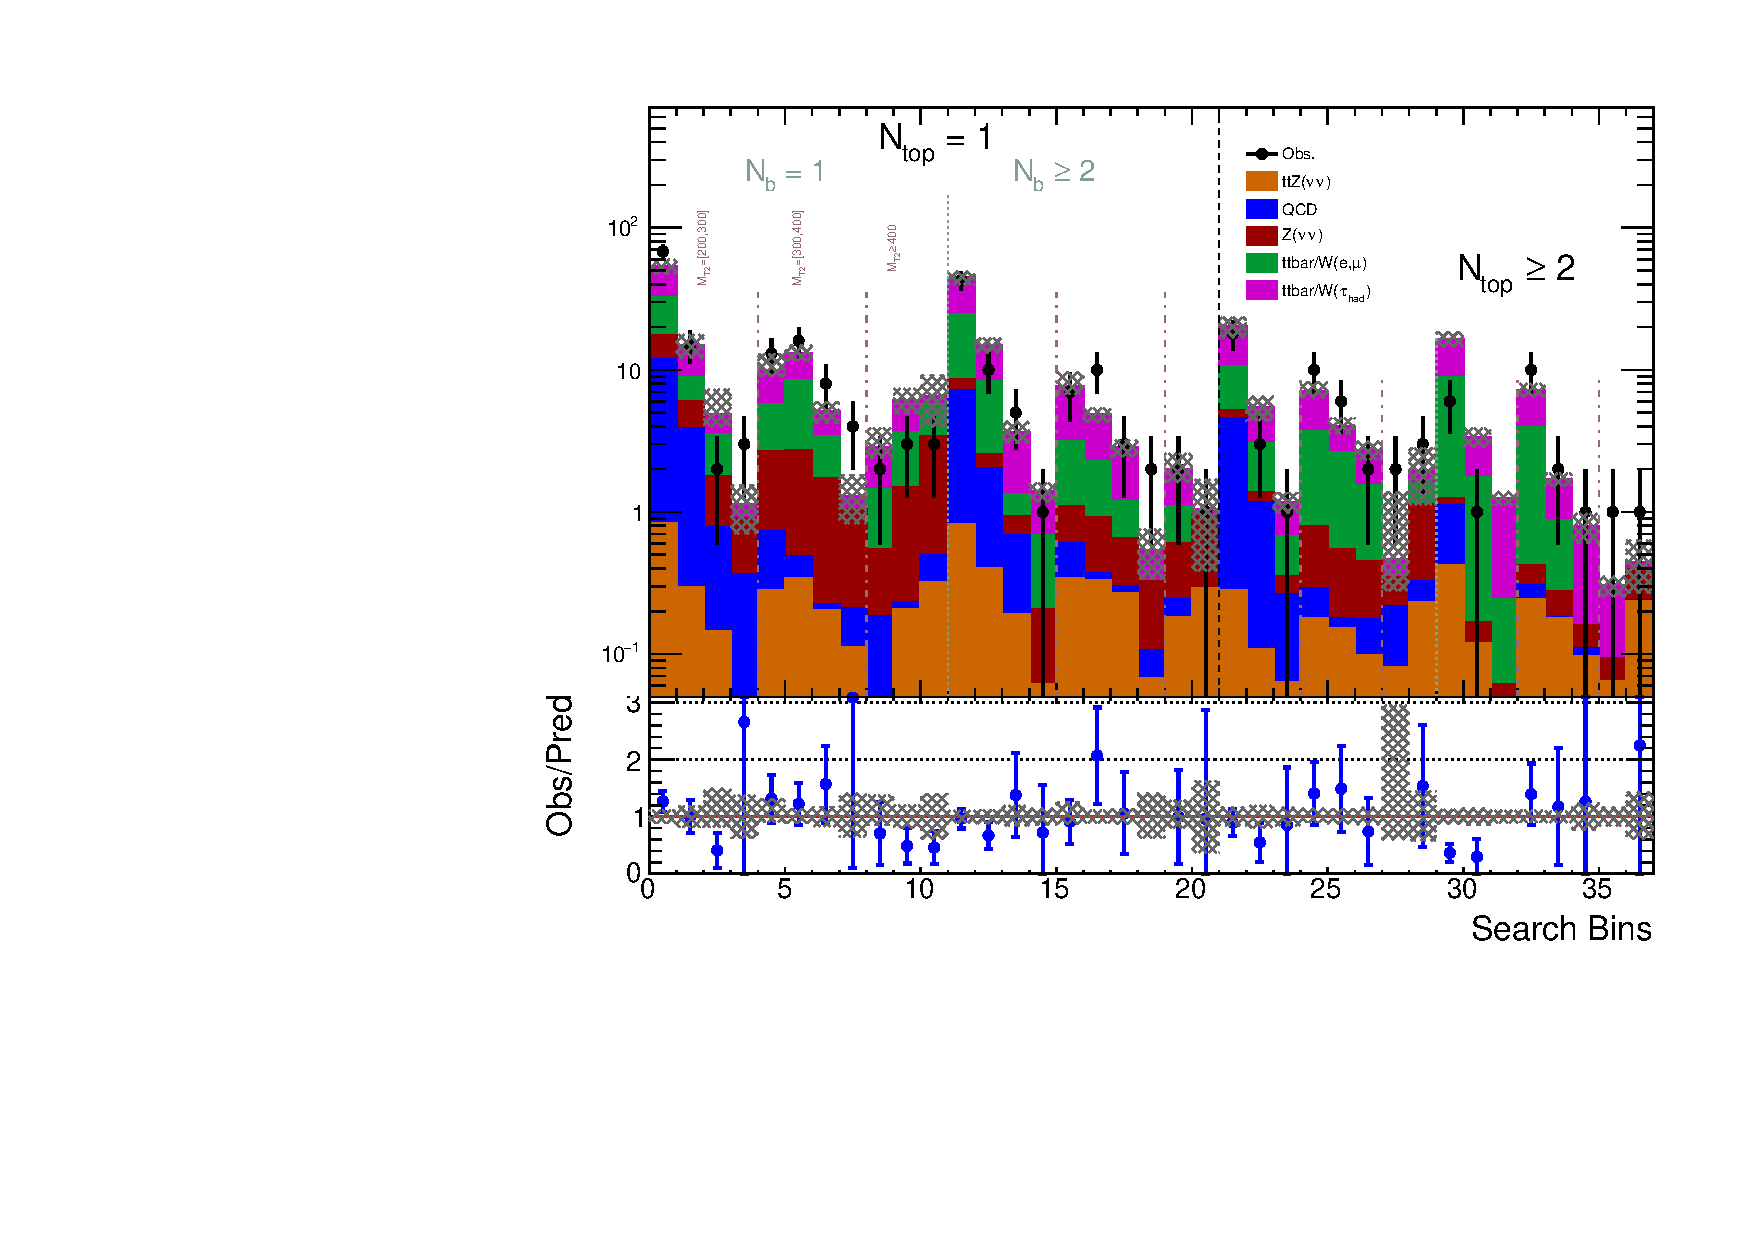
\includegraphics[angle=0,width=0.70\textwidth]{figures/UnblindPlots.pdf}
  \end{tabular}
  \caption{Data are shown as black points. The total predictions are shown in filled solid area. The bottom plot shows the ratio of data over total background prediction in each search bin. Only statistical uncertainties are propagated to the ratio.}
    \label{fig:baseline_SR}
  \end{center}
\end{figure}
%%%%%%%%%%%%%%%%%%%%%%%%%%%%%%%%%%%%%%%%%%%%%%%%%%

%%%%%%%%%%%%%%%%%%%%%%%%%%%%%%%%%%%%%%%%%%%%%%%%%%
\begin{landscape}
\newsavebox{\resBox}
\begin{table}[hp]
\centering
\caption{In the merged 37 bins: observed yields from the full luminosity of data compared to our total background predictions for the search bins.}
\label{tab:obs_vs_pred_37Bins}
\begin{lrbox}{\resBox}
%{\footnotesize
\begin{tabular}{|c|c|c|c|c||c|c||c|c|c|c|c|}
\hline
     SB &          \ntops &   \nbjets &   \MTTwo [\GeV] &     \MET [\GeV]  & Obs. & Sum. Pred. & Lost. Lep. & Had. Tau & Z($\nu\nu$)+Jets & QCD & ttZ \\
 \hline
              0 &               1 &               1 &         200-300 &         200-275  &     68 &  53.72 $^{+3.93}_{-3.78}$ $^{+6.44}_{-6.43}$ &  14.97 $^{+2.80}_{-2.63}$ $^{+2.23}_{-2.19}$ &  21.10 $^{+2.39}_{-2.32}$ $^{+1.39}_{-1.39}$ &   5.74 $^{+0.09}_{-0.09}$ $^{+1.56}_{-1.56}$ &  11.08 $^{+1.39}_{-1.39}$ $^{+5.66}_{-5.66}$ &   0.83 $^{+0.05}_{-0.05}$ $^{+0.29}_{-0.28}$ \\
 \hline
              1 &               1 &               1 &         200-300 &         275-350  &     15 &  14.95 $^{+2.18}_{-1.86}$ $^{+2.81}_{-2.81}$ &   2.84 $^{+1.57}_{-1.21}$ $^{+0.44}_{-0.44}$ &   6.15 $^{+1.29}_{-1.17}$ $^{+0.47}_{-0.47}$ &   2.11 $^{+0.05}_{-0.05}$ $^{+0.67}_{-0.67}$ &   3.56 $^{+0.80}_{-0.80}$ $^{+2.65}_{-2.65}$ &   0.30 $^{+0.03}_{-0.03}$ $^{+0.10}_{-0.10}$ \\
 \hline
              2 &               1 &               1 &         200-300 &         350-450  &      2 &   4.88 $^{+1.64}_{-1.16}$ $^{+2.44}_{-0.90}$ &   1.75 $^{+1.48}_{-1.07}$ $^{+0.30}_{-0.30}$ &   1.33 $^{+0.64}_{-0.33}$ $^{+0.18}_{-0.18}$ &   1.01 $^{+0.03}_{-0.03}$ $^{+0.53}_{-0.53}$ &   0.64 $^{+0.32}_{-0.32}$ $^{+2.35}_{-0.64}$ &   0.14 $^{+0.02}_{-0.02}$ $^{+0.05}_{-0.05}$ \\
 \hline
              3 &               1 &               1 &         200-300 &            450+  &      3 &   1.13 $^{+1.06}_{-0.23}$ $^{+0.43}_{-0.43}$ &   0.00 $^{+0.88}_{-0.00}$ $^{+0.00}_{-0.00}$ &   0.22 $^{+0.56}_{-0.09}$ $^{+0.03}_{-0.04}$ &   0.54 $^{+0.02}_{-0.02}$ $^{+0.29}_{-0.29}$ &   0.34 $^{+0.21}_{-0.21}$ $^{+0.31}_{-0.31}$ &   0.02 $^{+0.01}_{-0.01}$ $^{+0.01}_{-0.01}$ \\
 \hline
              4 &               1 &               1 &         300-400 &         200-275  &     13 &   9.90 $^{+1.84}_{-1.53}$ $^{+3.12}_{-0.97}$ &   3.02 $^{+1.47}_{-1.18}$ $^{+0.48}_{-0.47}$ &   4.18 $^{+1.11}_{-0.96}$ $^{+0.32}_{-0.32}$ &   1.96 $^{+0.05}_{-0.05}$ $^{+0.63}_{-0.63}$ &   0.45 $^{+0.09}_{-0.09}$ $^{+3.00}_{-0.45}$ &   0.28 $^{+0.03}_{-0.03}$ $^{+0.09}_{-0.09}$ \\
 \hline
              5 &               1 &               1 &         300-400 &         275-350  &     16 &  13.08 $^{+2.39}_{-2.09}$ $^{+1.78}_{-1.49}$ &   5.75 $^{+2.07}_{-1.80}$ $^{+0.92}_{-0.91}$ &   4.60 $^{+1.19}_{-1.06}$ $^{+0.75}_{-0.74}$ &   2.24 $^{+0.06}_{-0.06}$ $^{+0.89}_{-0.89}$ &   0.15 $^{+0.05}_{-0.05}$ $^{+0.97}_{-0.15}$ &   0.34 $^{+0.03}_{-0.03}$ $^{+0.12}_{-0.12}$ \\
 \hline
              6 &               1 &               1 &         300-400 &         350-450  &      8 &   5.09 $^{+1.70}_{-1.11}$ $^{+0.89}_{-0.88}$ &   1.65 $^{+1.51}_{-0.97}$ $^{+0.32}_{-0.32}$ &   1.71 $^{+0.77}_{-0.53}$ $^{+0.20}_{-0.20}$ &   1.51 $^{+0.04}_{-0.04}$ $^{+0.80}_{-0.80}$ &   0.02 $^{+0.05}_{-0.05}$ $^{+0.06}_{-0.02}$ &   0.20 $^{+0.03}_{-0.03}$ $^{+0.07}_{-0.07}$ \\
 \hline
              7 &               1 &               1 &         300-400 &            450+  &      4 &   1.30 $^{+1.08}_{-0.14}$ $^{+0.53}_{-0.47}$ &   0.00 $^{+0.91}_{-0.00}$ $^{+0.00}_{-0.00}$ &   0.25 $^{+0.56}_{-0.12}$ $^{+0.04}_{-0.04}$ &   0.84 $^{+0.03}_{-0.03}$ $^{+0.45}_{-0.45}$ &   0.10 $^{+0.07}_{-0.07}$ $^{+0.28}_{-0.10}$ &   0.11 $^{+0.02}_{-0.02}$ $^{+0.04}_{-0.04}$ \\
 \hline
              8 &               1 &               1 &            400+ &         200-350  &      2 &   2.83 $^{+1.28}_{-0.79}$ $^{+1.06}_{-0.43}$ &   0.91 $^{+0.99}_{-0.52}$ $^{+0.20}_{-0.19}$ &   1.38 $^{+0.81}_{-0.59}$ $^{+0.22}_{-0.22}$ &   0.36 $^{+0.02}_{-0.02}$ $^{+0.28}_{-0.28}$ &   0.15 $^{+0.05}_{-0.05}$ $^{+0.98}_{-0.15}$ &   0.04 $^{+0.01}_{-0.01}$ $^{+0.01}_{-0.01}$ \\
 \hline
              9 &               1 &               1 &            400+ &         350-450  &      3 &   6.16 $^{+2.12}_{-1.52}$ $^{+1.24}_{-1.24}$ &   2.15 $^{+1.85}_{-1.26}$ $^{+0.41}_{-0.40}$ &   2.51 $^{+1.02}_{-0.85}$ $^{+0.45}_{-0.45}$ &   1.26 $^{+0.04}_{-0.04}$ $^{+1.08}_{-1.08}$ &   0.02 $^{+0.05}_{-0.05}$ $^{+0.07}_{-0.02}$ &   0.21 $^{+0.03}_{-0.03}$ $^{+0.07}_{-0.07}$ \\
 \hline
             10 &               1 &               1 &            400+ &            450+  &      3 &   6.55 $^{+2.11}_{-1.45}$ $^{+2.64}_{-2.59}$ &   2.33 $^{+1.98}_{-1.37}$ $^{+0.48}_{-0.48}$ &   0.79 $^{+0.73}_{-0.47}$ $^{+0.12}_{-0.12}$ &   2.93 $^{+0.06}_{-0.06}$ $^{+2.53}_{-2.53}$ &   0.18 $^{+0.10}_{-0.10}$ $^{+0.52}_{-0.18}$ &   0.32 $^{+0.03}_{-0.03}$ $^{+0.11}_{-0.11}$ \\
 \hline
             11 &               1 &              2+ &         200-300 &         200-275  &     43 &  44.60 $^{+4.15}_{-4.00}$ $^{+4.82}_{-4.80}$ &  16.25 $^{+3.17}_{-3.02}$ $^{+2.48}_{-2.44}$ &  19.81 $^{+2.44}_{-2.38}$ $^{+1.33}_{-1.33}$ &   1.38 $^{+0.04}_{-0.04}$ $^{+0.96}_{-0.96}$ &   6.33 $^{+1.10}_{-1.10}$ $^{+3.78}_{-3.78}$ &   0.83 $^{+0.05}_{-0.05}$ $^{+0.27}_{-0.27}$ \\
 \hline
             12 &               1 &              2+ &         200-300 &         275-350  &     10 &  14.95 $^{+2.64}_{-2.35}$ $^{+1.80}_{-1.79}$ &   5.72 $^{+2.10}_{-1.80}$ $^{+0.89}_{-0.88}$ &   6.67 $^{+1.51}_{-1.40}$ $^{+0.49}_{-0.49}$ &   0.53 $^{+0.03}_{-0.03}$ $^{+0.39}_{-0.39}$ &   1.63 $^{+0.57}_{-0.57}$ $^{+1.43}_{-1.43}$ &   0.40 $^{+0.04}_{-0.04}$ $^{+0.14}_{-0.14}$ \\
 \hline
             13 &               1 &              2+ &         200-300 &         350-450  &      5 &   3.63 $^{+1.54}_{-0.89}$ $^{+0.71}_{-0.58}$ &   0.39 $^{+1.20}_{-0.39}$ $^{+0.07}_{-0.07}$ &   2.30 $^{+0.94}_{-0.76}$ $^{+0.21}_{-0.21}$ &   0.26 $^{+0.02}_{-0.02}$ $^{+0.21}_{-0.21}$ &   0.49 $^{+0.26}_{-0.26}$ $^{+0.64}_{-0.49}$ &   0.19 $^{+0.02}_{-0.02}$ $^{+0.07}_{-0.07}$ \\
 \hline
             14 &               1 &              2+ &         200-300 &            450+  &      1 &   1.39 $^{+1.48}_{-0.66}$ $^{+0.23}_{-0.21}$ &   0.48 $^{+1.30}_{-0.48}$ $^{+0.13}_{-0.13}$ &   0.71 $^{+0.71}_{-0.44}$ $^{+0.10}_{-0.10}$ &   0.14 $^{+0.01}_{-0.01}$ $^{+0.13}_{-0.13}$ &   0.00 $^{+0.13}_{-0.13}$ $^{+0.11}_{-0.00}$ &   0.06 $^{+0.01}_{-0.01}$ $^{+0.02}_{-0.02}$ \\
 \hline
             15 &               1 &              2+ &         300-400 &         200-275  &      7 &   7.68 $^{+1.75}_{-1.38}$ $^{+2.01}_{-0.95}$ &   2.06 $^{+1.25}_{-0.85}$ $^{+0.38}_{-0.38}$ &   4.53 $^{+1.22}_{-1.09}$ $^{+0.75}_{-0.75}$ &   0.49 $^{+0.03}_{-0.03}$ $^{+0.34}_{-0.34}$ &   0.26 $^{+0.06}_{-0.06}$ $^{+1.78}_{-0.26}$ &   0.34 $^{+0.03}_{-0.03}$ $^{+0.13}_{-0.12}$ \\
 \hline
             16 &               1 &              2+ &         300-400 &         275-350  &     10 &   4.83 $^{+1.70}_{-1.12}$ $^{+0.59}_{-0.54}$ &   1.36 $^{+1.39}_{-0.79}$ $^{+0.24}_{-0.24}$ &   2.55 $^{+0.96}_{-0.79}$ $^{+0.23}_{-0.23}$ &   0.55 $^{+0.03}_{-0.03}$ $^{+0.41}_{-0.41}$ &   0.04 $^{+0.03}_{-0.03}$ $^{+0.24}_{-0.04}$ &   0.33 $^{+0.03}_{-0.03}$ $^{+0.11}_{-0.11}$ \\
 \hline
             17 &               1 &              2+ &         300-400 &         350-450  &      3 &   2.83 $^{+1.61}_{-0.85}$ $^{+0.39}_{-0.38}$ &   0.54 $^{+1.37}_{-0.54}$ $^{+0.10}_{-0.10}$ &   1.64 $^{+0.86}_{-0.66}$ $^{+0.20}_{-0.20}$ &   0.35 $^{+0.02}_{-0.02}$ $^{+0.29}_{-0.29}$ &   0.03 $^{+0.05}_{-0.05}$ $^{+0.09}_{-0.03}$ &   0.27 $^{+0.03}_{-0.03}$ $^{+0.10}_{-0.09}$ \\
 \hline
             18 &               1 &              2+ &         300-400 &            450+  &      2 &   0.54 $^{+1.27}_{-0.15}$ $^{+0.23}_{-0.20}$ &   0.00 $^{+1.13}_{-0.00}$ $^{+0.00}_{-0.00}$ &   0.21 $^{+0.57}_{-0.13}$ $^{+0.03}_{-0.03}$ &   0.22 $^{+0.01}_{-0.01}$ $^{+0.19}_{-0.19}$ &   0.04 $^{+0.05}_{-0.05}$ $^{+0.11}_{-0.04}$ &   0.07 $^{+0.01}_{-0.01}$ $^{+0.02}_{-0.02}$ \\
 \hline
             19 &               1 &              2+ &            400+ &         200-450  &      2 &   2.01 $^{+1.42}_{-0.68}$ $^{+0.57}_{-0.40}$ &   0.49 $^{+1.22}_{-0.49}$ $^{+0.12}_{-0.12}$ &   0.92 $^{+0.72}_{-0.47}$ $^{+0.13}_{-0.13}$ &   0.36 $^{+0.02}_{-0.02}$ $^{+0.35}_{-0.35}$ &   0.06 $^{+0.03}_{-0.03}$ $^{+0.41}_{-0.06}$ &   0.18 $^{+0.02}_{-0.02}$ $^{+0.07}_{-0.06}$ \\
 \hline
             20 &               1 &              2+ &            400+ &            450+  &      1 &   1.04 $^{+1.77}_{-0.06}$ $^{+0.66}_{-0.65}$ &   0.00 $^{+1.68}_{-0.00}$ $^{+0.00}_{-0.00}$ &   0.09 $^{+0.55}_{-0.05}$ $^{+0.02}_{-0.02}$ &   0.66 $^{+0.02}_{-0.02}$ $^{+0.65}_{-0.65}$ &   0.00 $^{+0.07}_{-0.00}$ $^{+0.00}_{-0.00}$ &   0.29 $^{+0.03}_{-0.03}$ $^{+0.10}_{-0.10}$ \\
 \hline
             21 &              2+ &               1 &         200-300 &         200-275  &     18 &  20.13 $^{+2.43}_{-2.30}$ $^{+3.31}_{-3.30}$ &   5.42 $^{+1.68}_{-1.59}$ $^{+0.95}_{-0.92}$ &   9.50 $^{+1.53}_{-1.43}$ $^{+0.94}_{-0.94}$ &   0.67 $^{+0.03}_{-0.03}$ $^{+0.48}_{-0.48}$ &   4.27 $^{+0.87}_{-0.87}$ $^{+2.99}_{-2.99}$ &   0.28 $^{+0.03}_{-0.03}$ $^{+0.08}_{-0.09}$ \\
 \hline
             22 &              2+ &               1 &         200-300 &         275-350  &      3 &   5.47 $^{+1.38}_{-1.13}$ $^{+1.08}_{-1.08}$ &   1.69 $^{+0.94}_{-0.74}$ $^{+0.40}_{-0.39}$ &   2.41 $^{+0.91}_{-0.72}$ $^{+0.43}_{-0.43}$ &   0.20 $^{+0.01}_{-0.01}$ $^{+0.15}_{-0.15}$ &   1.07 $^{+0.44}_{-0.44}$ $^{+0.90}_{-0.90}$ &   0.11 $^{+0.02}_{-0.02}$ $^{+0.03}_{-0.03}$ \\
 \hline
             23 &              2+ &               1 &         200-300 &            350+  &      1 &   1.17 $^{+0.89}_{-0.50}$ $^{+0.20}_{-0.20}$ &   0.32 $^{+0.59}_{-0.32}$ $^{+0.07}_{-0.07}$ &   0.50 $^{+0.65}_{-0.34}$ $^{+0.08}_{-0.08}$ &   0.09 $^{+0.01}_{-0.01}$ $^{+0.08}_{-0.08}$ &   0.20 $^{+0.18}_{-0.18}$ $^{+0.15}_{-0.15}$ &   0.06 $^{+0.01}_{-0.01}$ $^{+0.02}_{-0.02}$ \\
 \hline
             24 &              2+ &               1 &         300-400 &         200-275  &     10 &   7.11 $^{+1.82}_{-1.52}$ $^{+1.06}_{-0.72}$ &   2.88 $^{+1.51}_{-1.26}$ $^{+0.48}_{-0.47}$ &   3.43 $^{+1.02}_{-0.86}$ $^{+0.39}_{-0.39}$ &   0.50 $^{+0.02}_{-0.02}$ $^{+0.37}_{-0.37}$ &   0.11 $^{+0.05}_{-0.05}$ $^{+0.77}_{-0.11}$ &   0.18 $^{+0.02}_{-0.02}$ $^{+0.05}_{-0.06}$ \\
 \hline
             25 &              2+ &               1 &         300-400 &         275-350  &      6 &   4.03 $^{+1.49}_{-1.08}$ $^{+0.53}_{-0.49}$ &   2.10 $^{+1.32}_{-0.99}$ $^{+0.37}_{-0.37}$ &   1.38 $^{+0.69}_{-0.41}$ $^{+0.15}_{-0.15}$ &   0.37 $^{+0.02}_{-0.02}$ $^{+0.28}_{-0.28}$ &   0.03 $^{+0.02}_{-0.02}$ $^{+0.21}_{-0.03}$ &   0.15 $^{+0.02}_{-0.02}$ $^{+0.05}_{-0.05}$ \\
 \hline
             26 &              2+ &               1 &         300-400 &            350+  &      2 &   2.70 $^{+1.18}_{-0.81}$ $^{+0.44}_{-0.38}$ &   1.08 $^{+0.92}_{-0.65}$ $^{+0.24}_{-0.24}$ &   1.17 $^{+0.73}_{-0.48}$ $^{+0.15}_{-0.16}$ &   0.28 $^{+0.02}_{-0.02}$ $^{+0.23}_{-0.23}$ &   0.08 $^{+0.07}_{-0.07}$ $^{+0.23}_{-0.08}$ &   0.10 $^{+0.02}_{-0.02}$ $^{+0.03}_{-0.03}$ \\
 \hline
             27 &              2+ &               1 &            400+ &         200-350  &      2 &   0.47 $^{+1.09}_{-0.13}$ $^{+0.92}_{-0.19}$ &   0.00 $^{+0.93}_{-0.00}$ $^{+0.00}_{-0.00}$ &   0.12 $^{+0.56}_{-0.12}$ $^{+0.02}_{-0.02}$ &   0.13 $^{+0.01}_{-0.01}$ $^{+0.12}_{-0.12}$ &   0.14 $^{+0.04}_{-0.04}$ $^{+0.91}_{-0.14}$ &   0.08 $^{+0.02}_{-0.02}$ $^{+0.03}_{-0.03}$ \\
 \hline
             28 &              2+ &               1 &            400+ &            350+  &      3 &   1.95 $^{+1.11}_{-0.51}$ $^{+0.88}_{-0.83}$ &   0.45 $^{+0.93}_{-0.45}$ $^{+0.09}_{-0.09}$ &   0.36 $^{+0.59}_{-0.22}$ $^{+0.07}_{-0.07}$ &   0.81 $^{+0.03}_{-0.03}$ $^{+0.82}_{-0.81}$ &   0.10 $^{+0.09}_{-0.09}$ $^{+0.28}_{-0.10}$ &   0.23 $^{+0.03}_{-0.03}$ $^{+0.07}_{-0.07}$ \\
 \hline
             29 &              2+ &              2+ &         200-300 &         200-275  &      6 &  16.41 $^{+2.90}_{-2.79}$ $^{+2.05}_{-2.02}$ &   7.62 $^{+2.50}_{-2.43}$ $^{+1.61}_{-1.56}$ &   7.54 $^{+1.40}_{-1.28}$ $^{+1.13}_{-1.13}$ &   0.14 $^{+0.01}_{-0.01}$ $^{+0.11}_{-0.11}$ &   0.69 $^{+0.45}_{-0.45}$ $^{+0.57}_{-0.57}$ &   0.43 $^{+0.04}_{-0.04}$ $^{+0.14}_{-0.14}$ \\
 \hline
             30 &              2+ &              2+ &         200-300 &         275-350  &      1 &   3.38 $^{+1.33}_{-1.06}$ $^{+0.55}_{-0.52}$ &   1.58 $^{+1.03}_{-0.85}$ $^{+0.44}_{-0.43}$ &   1.63 $^{+0.81}_{-0.59}$ $^{+0.27}_{-0.27}$ &   0.05 $^{+0.01}_{-0.01}$ $^{+0.04}_{-0.04}$ &   0.00 $^{+0.23}_{-0.23}$ $^{+0.17}_{-0.00}$ &   0.12 $^{+0.02}_{-0.02}$ $^{+0.04}_{-0.04}$ \\
 \hline
             31 &              2+ &              2+ &         200-300 &            350+  &      0 &   1.25 $^{+0.89}_{-0.44}$ $^{+0.15}_{-0.14}$ &   0.18 $^{+0.58}_{-0.18}$ $^{+0.04}_{-0.04}$ &   1.01 $^{+0.67}_{-0.38}$ $^{+0.13}_{-0.13}$ &   0.02 $^{+0.00}_{-0.00}$ $^{+0.02}_{-0.02}$ &   0.00 $^{+0.09}_{-0.09}$ $^{+0.06}_{-0.00}$ &   0.04 $^{+0.01}_{-0.01}$ $^{+0.01}_{-0.01}$ \\
 \hline
             32 &              2+ &              2+ &         300-400 &         200-275  &     10 &   7.18 $^{+1.80}_{-1.50}$ $^{+0.84}_{-0.70}$ &   3.51 $^{+1.41}_{-1.14}$ $^{+0.62}_{-0.60}$ &   3.24 $^{+1.12}_{-0.97}$ $^{+0.32}_{-0.32}$ &   0.12 $^{+0.01}_{-0.01}$ $^{+0.10}_{-0.10}$ &   0.06 $^{+0.04}_{-0.04}$ $^{+0.46}_{-0.06}$ &   0.24 $^{+0.03}_{-0.03}$ $^{+0.08}_{-0.08}$ \\
 \hline
             33 &              2+ &              2+ &         300-400 &         275-350  &      2 &   1.70 $^{+1.28}_{-0.67}$ $^{+0.18}_{-0.18}$ &   0.60 $^{+1.11}_{-0.60}$ $^{+0.11}_{-0.11}$ &   0.83 $^{+0.63}_{-0.31}$ $^{+0.10}_{-0.10}$ &   0.09 $^{+0.01}_{-0.01}$ $^{+0.08}_{-0.08}$ &   0.00 $^{+0.02}_{-0.02}$ $^{+0.02}_{-0.00}$ &   0.18 $^{+0.02}_{-0.02}$ $^{+0.06}_{-0.06}$ \\
 \hline
             34 &              2+ &              2+ &         300-400 &            350+  &      1 &   0.79 $^{+1.00}_{-0.33}$ $^{+0.19}_{-0.19}$ &   0.00 $^{+0.77}_{-0.00}$ $^{+0.00}_{-0.00}$ &   0.63 $^{+0.64}_{-0.33}$ $^{+0.18}_{-0.18}$ &   0.05 $^{+0.01}_{-0.01}$ $^{+0.04}_{-0.04}$ &   0.01 $^{+0.04}_{-0.04}$ $^{+0.04}_{-0.01}$ &   0.10 $^{+0.02}_{-0.02}$ $^{+0.03}_{-0.03}$ \\
 \hline
             35 &              2+ &              2+ &            400+ &         200-350  &      1 &   0.30 $^{+1.00}_{-0.16}$ $^{+0.05}_{-0.05}$ &   0.00 $^{+0.82}_{-0.00}$ $^{+0.00}_{-0.00}$ &   0.21 $^{+0.57}_{-0.16}$ $^{+0.03}_{-0.03}$ &   0.03 $^{+0.00}_{-0.00}$ $^{+0.03}_{-0.03}$ &   0.00 $^{+0.02}_{-0.00}$ $^{+0.01}_{-0.00}$ &   0.06 $^{+0.01}_{-0.01}$ $^{+0.02}_{-0.02}$ \\
 \hline
             36 &              2+ &              2+ &            400+ &            350+  &      1 &   0.44 $^{+1.27}_{-0.06}$ $^{+0.19}_{-0.18}$ &   0.00 $^{+1.14}_{-0.00}$ $^{+0.00}_{-0.00}$ &   0.05 $^{+0.55}_{-0.04}$ $^{+0.01}_{-0.01}$ &   0.16 $^{+0.01}_{-0.01}$ $^{+0.17}_{-0.16}$ &   0.00 $^{+0.04}_{-0.04}$ $^{+0.02}_{-0.00}$ &   0.23 $^{+0.03}_{-0.03}$ $^{+0.08}_{-0.08}$ \\
 \hline
\end{tabular}
%\footnotesize}
\end{lrbox}
\scalebox{0.80}{\usebox{\resBox}}
\end{table}
\end{landscape}

%%%%%%%%%%%%%%%%%%%%%%%%%%%%%%%%%%%%%%%%%%%%%%%%%%
Table~\ref{tab:obs_vs_pred_37Bins} details the observed data and the total background prediction, together with their statistical and systematic uncertainties. 
%
As can be seen, good agreement is observed between the SM background predictions and the yields observed in data for each search bin, within uncertainties.
%
%%%%%%%%%%%%%%%%%%%%%%%%%%%%%%%%%%%%%%%%%%%%%%%%%%
%\subsection{Interpretation in terms of direct pair production of scalar top quarks}
%%%%%%%%%%%%%%%%%%%%%%%%%%%%%%%%%%%%%%%%%%%%%%%%%%
%
Because the observed data yields are consistent with SM expectations.
%
A modified frequentist CLs method is used taking a profile likelihood as a test statistic~\cite{aread,tjunk,ATL-PHYS-PUB-2011-011} in order to determine the upper limit on the possible contributions from non-SM processes in this search. 
%
In particular, these results are used to set limits on the T2tt and T2tb signal models for scalar top quark pair production. 
%
The cross sections are determined at the NLO in the strong coupling constant and include the resummation of soft gluon emission at the accuracy of next-to-leading-log (NLL) level~\cite{bib-nlo-nll-01,bib-nlo-nll-02,bib-nlo-nll-03,bib-nlo-nll-04,bib-nlo-nll-05,SMSXsecUnc}.

%-------------
The following uncertainties on the signal modelling are taken into account when the limits are determined: simulation sample size, luminosity determination ($4.6\%$), lepton and isolated track veto, b-tag efficiency corrections used to scale simulation to data, trigger efficiency, QCD renormalisation and factorisation scales, initial/final state radiation (ISR/FSR), signal acceptance and efficiency arising from the jet energy-momentum corrections, jet energy-momentum resolutions, and propagated to \MET, parton distribution functions (PDF) of the proton, and uncertainties in the faithfulness of the fast-simulation compared with the full-simulation for top-quark reconstruction and mistagging.  
%
The typical values of these systematic effects are listed in Tab.~\ref{tab:sigSyst}
%
The effect of potential contributions of signal events in the control data regions used to predict the backgrounds in each search bin are included. 
%
%%%%%%%%%%%%%%%%%%%%%%%%%%%%%%%%%%%%%%%%%%%%%%%%%%
\begin{table}[hp]
\centering
\caption{Sources of signal systematic uncertainties and their typical ranges. The last column indicates if the uncertainty across signal bins is correlated.}
\label{tab:sigSyst}
\begin{tabular}{l|c|c}
\hline \hline
Source & Typical Values & Correlated \\
\hline
MC statistics & 1-100\% & No \\
\hline
Luminosity & 2.7\% &  Yes \\
\hline
Renormalization and factorization scales & 0-2.6\% & Yes \\
\hline
``ISR'' recoil & 0-30\% & Yes \\
\hline
b-tagging efficiency, heavy flavor & 0-31\% & Yes \\
\hline
b-tagging efficiency, light flavor & 0-36\% & Yes \\
\hline
Lepton veto & 0-3.3\% & Yes \\
\hline
Jet energy scale & 0-25\% & Yes \\
\hline
MET uncerntainty & 0-21\% & Yes \\
\hline
Trigger & 0-1\% & Yes \\
\hline
Full/fastsim scale for top reco. & 0-5\% & Yes \\
\hline
top mistag uncertainty & 0-5\% & Yes \\
\hline
top tagger efficiency data/MC difference & 5\% & Yes \\
\hline \hline
\end{tabular}
\end{table}
%%%%%%%%%%%%%%%%%%%%%%%%%%%%%%%%%%%%%%%%%%%%%%%%%%

%-------------
The observed cross section upper limits on signal models of direct top squark pair production, T2tt and T2tb, are shown in Figure~\ref{fig:fulllimit_T2tt_T2tb}, together with contours that correspond to points for which the observed (black contour) and expected (red-dashed contour) upper limits equal the theoretical signal cross sections.
%%%%%%%%%%%%%%%%%%%%%%%%%%%%%%%%%%%%%%%%%%%%%%%%%%
\begin{figure}[htbp]
  \begin{center}
  \begin{tabular}{cc}
\hspace{-1.5cm}
  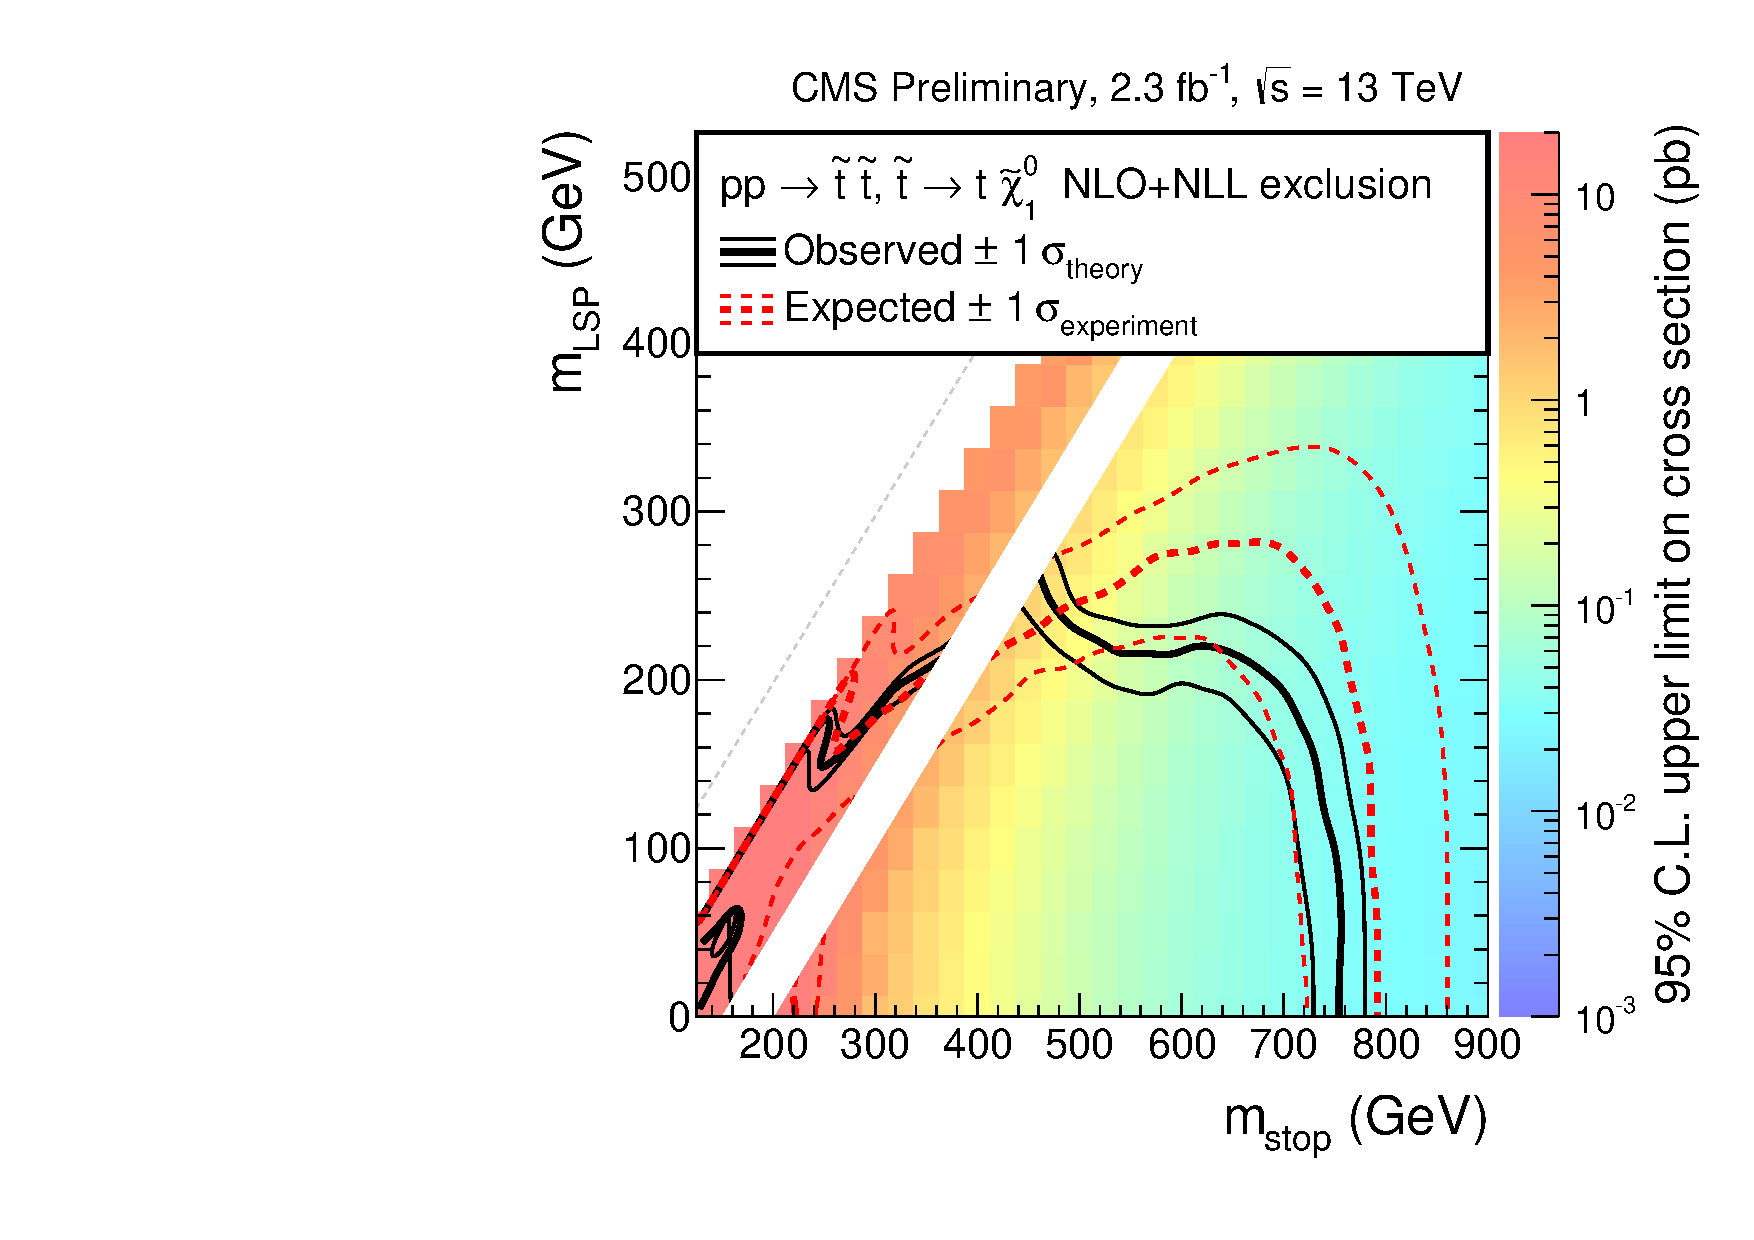
\includegraphics[angle=0,width=0.48\textwidth]{figures/Covered_BR_1p00_Stop_OnlyXSEC.pdf}
  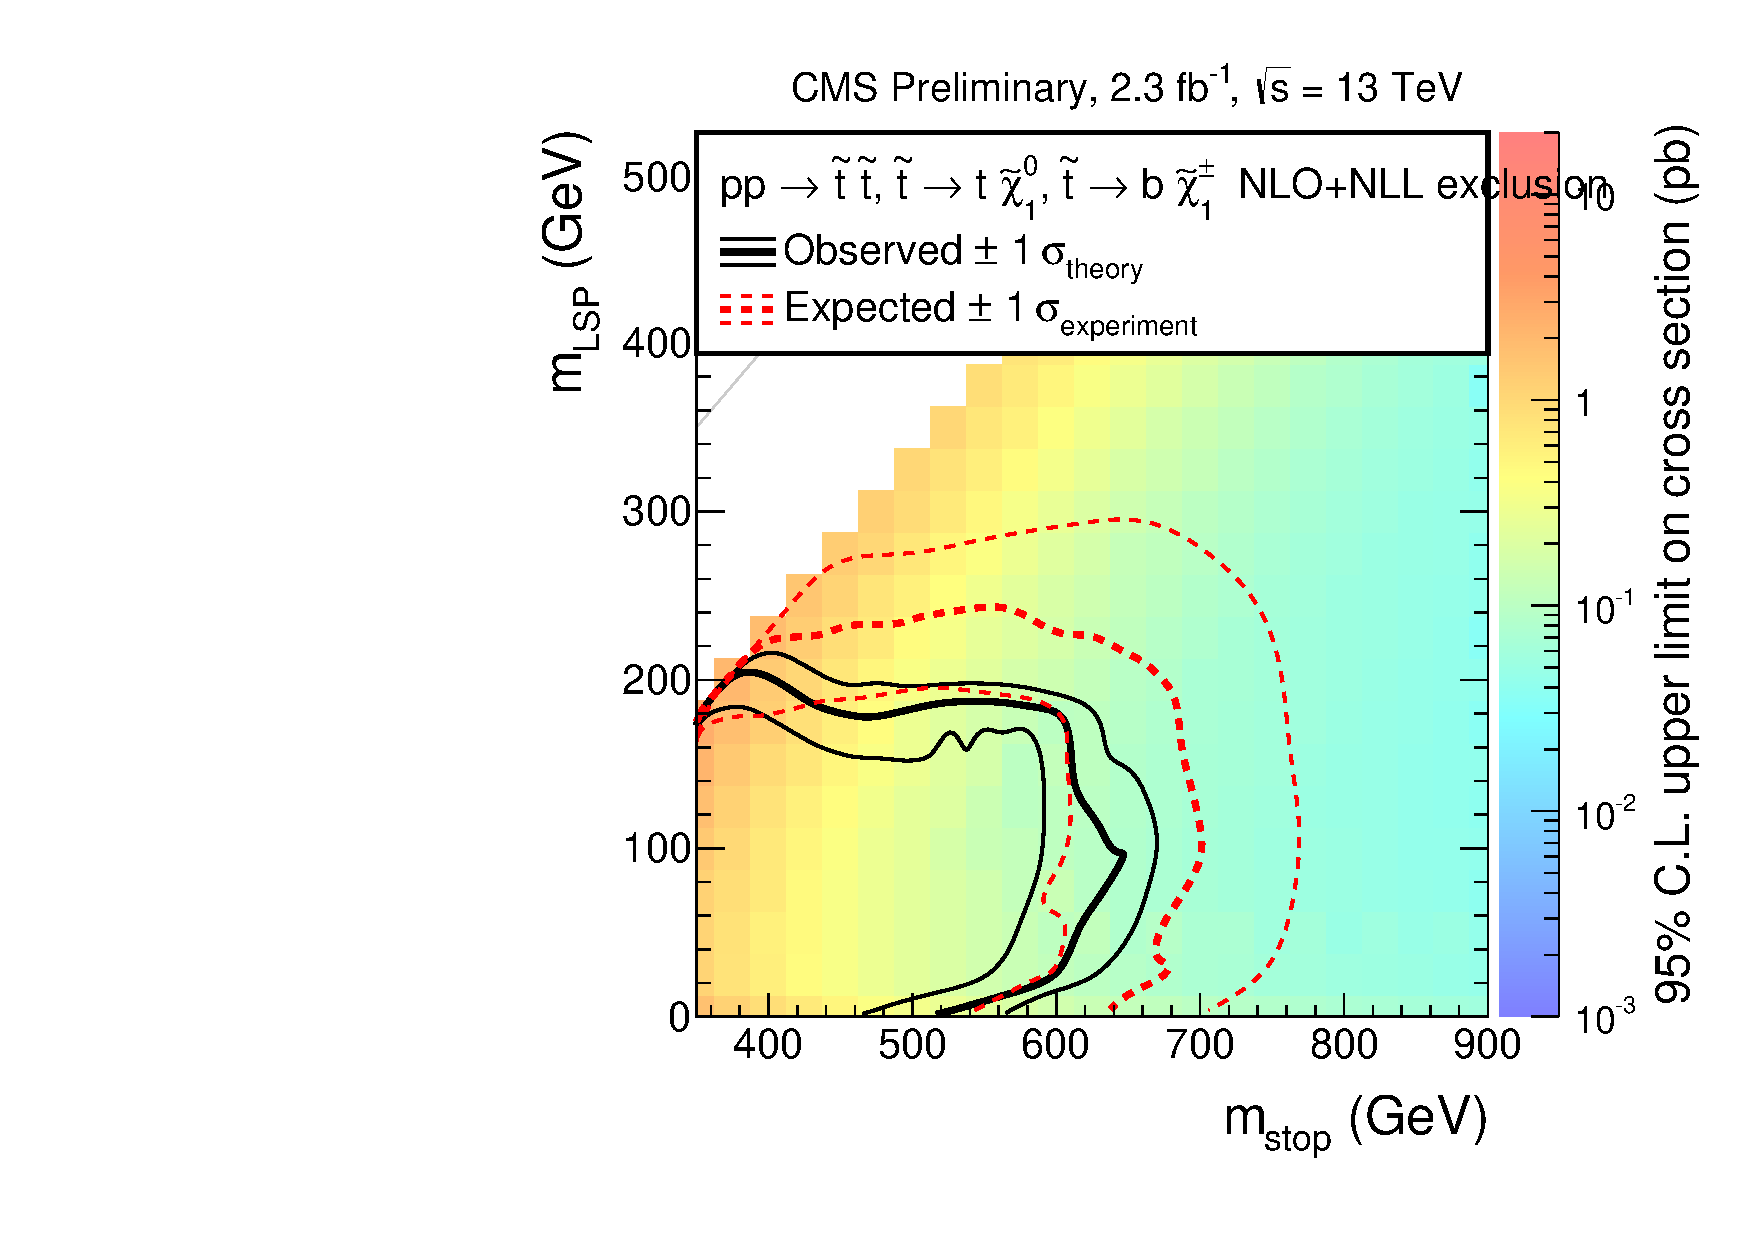
\includegraphics[angle=0,width=0.48\textwidth]{figures/BR_0p50_Stop_OnlyXSEC.pdf}
  \end{tabular}
  \caption{Expected limits and observed limits. The left shows the limits on the T2tt model, where the branching ratio for the top squark to decay to a top quark and neutralino is 100\%. The right plots shows the limits on the T2tb model, where the branching ratio for a top squark to decay to a top quark and neutralino is 50\%. }
    \label{fig:fulllimit_T2tt_T2tb}
  \end{center}
\end{figure}
%%%%%%%%%%%%%%%%%%%%%%%%%%%%%%%%%%%%%%%%%%%%%%%%%%
The observed exclusion curves are also shown for the cases in which the signal cross section is varied by changing the renormalization and factorization scales by a factor of 2 and using the PDF4LHC recommendation~\cite{Botje:2011sn} for the PDF uncertainty to illustrate the sensitivity of the exclusion to the signal cross section uncertainty.
%
The expected exclusion curves show the cases in which the background uncertainties are varied by one standard deviation.

In the T2tt model, shown in the left plot of Fig.~\ref{fig:fulllimit_T2tt_T2tb}, where both top squarks decay to top quarks and neutralinos, the median expected lower limit on the top squark mass reaches 790~\GeV, for small neutralino masses, and the observed limit excludes top squark masses below about 760~\GeV at 95\% confidence level.  
%
For large neutralino masses in the same model, the median expected lower mass limit on the neutralino reaches about 280~\GeV with an observed limit near 220~\GeV, for a top squark mass near 650~\GeV. 

In the T2tb model, displayed in the right plot f Fig.~\ref{fig:fulllimit_T2tt_T2tb}, which includes a light chargino (nearly degenerate with the neutralino) and allows the top squark to decay to a bottom quark and chargino with 50\% probability, the median expected lower limit reaches 700~\GeV, for a neutralino mass near 100~\GeV, and the observed limit excludes top squark masses below about 650~\GeV at 95\% confidence level. 
%
For larger neutralino masses, the median expected lower limit on the neutralino mass reaches about 240~\GeV with an observed limit near 200~\GeV. 










\section{Conclusions}

The results of a search for direct pair production of supersymmetric scalar top quarks in the all-hadronic final state has been performed.  
%
The top squarks may decay directly to stable neutralinos and top quarks, or may decay to charginos (nearly degenerate with the neutralinos) and bottom quarks.  
%
Top squark decay branching fractions to a top quark and neutralino of 100\% and 50\% have been studied.  
%
The data sample analyzed corresponds to 2.3~\fbinv of proton-proton collisions collected at a center-of-mass energy of 13~TeV by the CMS detector at the CERN LHC.  

No significant deviations beyond the Standard Model are observed and exclusion limits at 95\% confidence are set.  
%
In the case where both top squarks decay to top quarks and neutralinos, the median expected lower limit on the top squark mass reaches 800~\GeV, for small neutralino masses, and the observed limit excludes top squark masses below about 770~\GeV at 95\% confidence level.  
%
For large neutralino masses in the same model, the median expected lower mass limit on the neutralino reaches about 280~\GeV with an observed limit near 240~\GeV, for a top squark mass near 650~\GeV. 
%
In the case which includes a light chargino (nearly degenerate with the neutralino), allowing the top squark to decay to a bottom quark and chargino with 50\% probability, the median expected lower limit reaches 700~\GeV, for a neutralino mass near 100~\GeV, and the observed limit excludes top squark masses below about 670~\GeV at 95\% confidence level. 
%
For larger neutralino masses, the median expected lower limit on the neutralino mass reaches about 240~\GeV with an observed limit near 200~\GeV. 



%% **DO NOT REMOVE BIBLIOGRAPHY**
\bibliography{auto_generated}   % will be created by the tdr script.

%% examples of appendices. **DO NOT PUT \end{document} at the end
\clearpage
\appendix
\section{Analysis Cut Flow}
\label{sec:appendixcutflow}

\begin{table}[htb]
  \caption{Sample selection cut flow and event yields from MC simulated 
samples. All numbers are normalized to $2.2\fbinv$. 
Only statistical uncertainties are shown. Rare process refer to 
ttW, di-boson and tri-boson events.}
  \label{tab:cutflowMC1}
  \vskip-5ex
  \begin{center}
    \begin{tabular}{|c|c|c|c|c|}
      \hline
      Samples    & \ttbar          & \wlnu             & single top       & \znunu             \\
      Cuts       &                 &                   &                  &                    \\
      \hline
     No cut    & $9.77\times 10^5$ (100\%) & $4.62\times10^6$ (100\%) & $1.53\times10^5$ (100\%) & $9.88\times10^5$ (100\%)  \\
     \hline
  event filter & $9.64\times 10^5$  (99\%) & $4.54\times10^6$  (98\%) & $1.52\times10^5$  (99\%) & $9.81\times10^5$  (99\%)   \\
     \hline
   $\mu$ veto    & $6.18\times 10^5$ (64\%) & $3.39\times10^6$ (75\%) & $1.21\times10^5$ (80\%) & $9.80\times10^5$ (100\%)   \\
     \hline
       e veto    & $3.46\times 10^5$ (56\%) & $2.35\times10^6$ (69\%) & $9.69\times10^4$ (80\%) & $9.77\times10^5$ (100\%)   \\
     \hline
  isoTrk veto    & $2.20\times 10^5$ (63\%) & $1.81\times10^6$ (77\%) & $7.65\times10^4$ (79\%) & $9.34\times10^5$ (96\%)   \\
     \hline
$\njets\ge4$     & $1.04\times 10^5$ (48\%) & $8.21\times10^4$ (5\%) & $3.61\times10^4$ (47\%) & $3.38\times10^4$ (4\%)   \\
     \hline
$\nbjets\ge1$    & $8.49\times 10^4$ (81\%) & $1.23\times10^4$ (15\%) & $2.52\times10^4$ (70\%) & $5.72\times10^3$ (17\%)   \\
     \hline
$\HT\ge500$ GeV   & $1.63\times 10^4$ (19\%) & $2.99\times10^3$ (24\%) & $5.53\times10^3$ (22\%) & $1.50\times10^3$ (26\%)   \\
     \hline
$\met\ge200$ GeV & $1727\pm3$ (11\%) & $333\pm3$ (11\%) & $111\pm3$ (2\%) & $395\pm3$ (26\%)  \\
     \hline
 $\Delta\phi$    & $988\pm3$ (57\%) & $195\pm3$ (59\%) & $53\pm2$ (48\%) & $283\pm2$ (72\%)   \\
     \hline
tagger + $\ntops\ge1$ & $451\pm2$ (46\%) & $33\pm1$ (17\%) & $17\pm1$ (32\%) & $48\pm1$ (17\%)   \\
     \hline
$\MTTwo\ge200$ GeV & $289\pm1$ (64\%) & $28\pm1$ (83\%) & $13\pm1$ (77\%) & $42\pm1$ (87\%) \\
      \hline
    \end{tabular}
  \end{center}
\end{table}

\begin{table}[htb]
  \caption{Sample selection cut flow and event yields from MC simulated 
samples. All numbers are normalized to $2.2\fbinv$. 
Only statistical uncertainties are shown. Rare process refer to 
ttW, di-boson and tri-boson events.}
  \label{tab:cutflowMC2}
  \vskip-5ex
  \begin{center}
    \begin{tabular}{|c|c|c|c|c|}
      \hline
      Samples    & QCD          &  ttZ       &  rare          &  sum SM      \\
      Cuts       &              &            &                &          \\
      \hline
     No cut     & $6.39\times10^{10}$ (100\%) & $1.69\times10^3$ (100\%) & $3.87\times10^5$ (100\%) & $6.39\times10^{10}$ (100\%)  \\
     \hline
  event filter  & $6.34\times10^{10}$  (99\%) & $1.66\times10^3$  (99\%) & $3.81\times10^5$  (99\%) & $6.34\times10^{10}$ (99\%)  \\
     \hline
   $\mu$ veto    & $6.34\times10^{10}$ (100\%) & $1.26\times10^3$ (76\%) & $3.27\times10^5$ (86\%) & $6.34\times10^{10}$ (100\%)  \\
     \hline
       e veto    & $6.33\times10^{10}$ (100\%) & $9.61\times10^2$ (76\%) & $2.82\times10^5$ (86\%) & $6.33\times10^{10}$ (100\%)  \\
     \hline
  isoTrk veto     & $6.06\times10^{10}$ (96\%) & $7.30\times10^2$ (76\%) & $2.41\times10^5$ (85\%) & $6.06\times10^{10}$ (96\%)  \\
     \hline
$\njets\ge4$      & $5.65\times10^8$ (1\%) & $6.43\times10^2$ (88\%) & $1.96\times10^4$ (8\%) & $5.65\times10^8$ (1\%)  \\
     \hline
$\nbjets\ge1$     & $8.49\times10^7$ (15\%) & $5.21\times10^2$ (81\%) & $4.52\times10^3$ (23\%) & $8.50\times10^7$ (15\%)  \\
     \hline
$\HT\ge500$ GeV   & $6.46\times10^6$ (8\%) & $2.74\times10^2$ (53\%) & $9.59\times10^2$ (21\%) & $6.49\times10^6$ (8\%)  \\
     \hline
$\met\ge200$ GeV  & $6773\pm1053$ (0\%) & $21.7\pm0.4$ (8\%) & $27\pm2$ (3\%) & $9386\pm1053$ (0\%)  \\
     \hline
 $\Delta\phi$     & $1051\pm729$ (16\%) & $16.6\pm0.4$ (76\%) & $16\pm1$ (60\%) & $2604\pm729$ (28\%)  \\
     \hline
tagger + $\ntops\ge1$  & $52\pm6$ (5\%) & $9.0\pm0.3$ (54\%) & $4.5\pm0.6$ (28\%) & $615\pm7$ (24\%)  \\
     \hline
$\MTTwo\ge200$ GeV & $39\pm5$ (75\%) & $7.9\pm0.3$ (89\%) & $3.5\pm0.5 (76\%) $ & $422\pm6$ (69\%)  \\
      \hline
    \end{tabular}
  \end{center}
\end{table}

\begin{table}[htb]
  \caption{Sample selection cut flow and event yields from MC simulated 
samples. All numbers are normalized to $2.2\fbinv$. 
Only statistical uncertainties are shown. Rare process refer to 
ttW, di-boson and tri-boson events.}
  \label{tab:cutflowMC3}
  \vskip-5ex
  \begin{center}
    \begin{tabular}{|c|c|c|}
      \hline
      Samples    & T2tt        & T2tt         \\
      Cuts       & (500, 325)  & (850, 100)  \\
      \hline
     No cut      & $1.12\times10^3$ (100\%)  & $41$ (100\%)    \\
     \hline
  event filter   & $1.11\times10^3$ (99\%)  & $40$ (99\%)    \\
     \hline
   $\mu$ veto    & $8.75\times10^2$ (79\%) & 32 (79\%)    \\
     \hline
       e veto     & $6.92\times10^2$ (79\%)  & 25 (78\%)    \\
     \hline
  isoTrk veto     & $5.52\times10^2$ (80\%)  & 23 (93\%)    \\
     \hline
$\njets\ge4$     & $4.50\times10^2$ (81\%)  & 21 (90\%)    \\
     \hline
$\nbjets\ge1$      & $3.65\times10^2$ (81\%)  & 17 (83\%)    \\
     \hline
$\HT\ge500$ GeV    & $1.27\times10^2$ (35\%)  & 16 (94\%)    \\
     \hline
$\met\ge200$ GeV   & $52.9\pm0.4$ (42\%)  & $14.4\pm0.1$ (88\%)    \\
     \hline
 $\Delta\phi$      & $32.9\pm0.3$ (62\%)  & $13.0\pm0.1$ (91\%)    \\
     \hline
tagger + $\ntops\ge1$  & $18.6\pm0.2$ (57\%)  & $8.56\pm 0.04$ (66\%)    \\
     \hline
$\MTTwo\ge200$ GeV  & $14.9\pm0.2$ (80\%)  & $8.39\pm0.04$ (98\%)    \\
      \hline
    \end{tabular}
  \end{center}
\end{table}


\clearpage
\section{Background Predictions}
\label{sec:bkgpred}

\begin{table}[htbp]
\fontsize{10 pt}{1.2 em}
\selectfont
\begin{centering}
\caption{\label{tab:LLpred37} Predicted lost lepton background yield with
statistical and systematic uncertainties for a $2.3$~fb$^{-1}$ sample, in the case of 37 bins.}
\hspace*{-4ex}
\begin{lrbox}{\closureBox}
\begin{tabular}{|c|c|c|c|c||c|}
\hline
Search Bin & \ntops & \nbjets & \MTTwo [\GeV] & \MET [\GeV] & Lost Lepton Prediction\\
\hline
0 & 1 & 1 & 200-300 & 200-275 & 15.42 $^{+2.77}_{-2.61}$ $^{+2.29}_{-2.24}$ \\ 
\hline
1 & 1 & 1 & 200-300 & 275-350 & 2.69 $^{+1.50}_{-1.15}$ $^{+0.43}_{-0.42}$ \\ 
\hline
2 & 1 & 1 & 200-300 & 350-450 & 1.77 $^{+1.51}_{-1.08}$ $^{+0.27}_{-0.27}$ \\ 
\hline
3 & 1 & 1 & 200-300 & 450+ & 0 $^{+0.80}_{-0}$ $^{+0}_{-0}$ \\ 
\hline
4 & 1 & 1 & 300-400 & 200-275 & 3.03 $^{+1.49}_{-1.18}$ $^{+0.46}_{-0.45}$ \\ 
\hline
5 & 1 & 1 & 300-400 & 275-350 & 5.68 $^{+2.05}_{-1.78}$ $^{+0.86}_{-0.84}$ \\ 
\hline
6 & 1 & 1 & 300-400 & 350-450 & 1.22 $^{+1.16}_{-0.72}$ $^{+0.21}_{-0.21}$ \\ 
\hline
7 & 1 & 1 & 300-400 & 450+ & 0 $^{+0.95}_{-0}$ $^{+0}_{-0}$ \\ 
\hline
8 & 1 & 1 & 400+ & 200-350 & 0.82 $^{+0.89}_{-0.48}$ $^{+0.15}_{-0.15}$ \\ 
\hline
9 & 1 & 1 & 400+ & 350-450 & 1.76 $^{+1.57}_{-1.03}$ $^{+0.29}_{-0.28}$ \\ 
\hline
10 & 1 & 1 & 400+ & 450+ & 1.86 $^{+1.62}_{-1.09}$ $^{+0.31}_{-0.31}$ \\ 
\hline
11 & 1 & 2+ & 200-300 & 200-275 & 16.49 $^{+3.17}_{-3.02}$ $^{+2.51}_{-2.46}$ \\ 
\hline
12 & 1 & 2+ & 200-300 & 275-350 & 5.36 $^{+1.99}_{-1.68}$ $^{+0.77}_{-0.76}$ \\ 
\hline
13 & 1 & 2+ & 200-300 & 350-450 & 0 $^{+1.15}_{-0}$ $^{+0}_{-0}$ \\ 
\hline
14 & 1 & 2+ & 200-300 & 450+ & 0.42 $^{+1.16}_{-0.416}$ $^{+0.18}_{-0.18}$ \\ 
\hline
15 & 1 & 2+ & 300-400 & 200-275 & 2.17 $^{+1.31}_{-0.89}$ $^{+0.35}_{-0.34}$ \\ 
\hline
16 & 1 & 2+ & 300-400 & 275-350 & 1.21 $^{+1.26}_{-0.70}$ $^{+0.19}_{-0.19}$ \\ 
\hline
17 & 1 & 2+ & 300-400 & 350-450 & 0.58 $^{+1.43}_{-0.58}$ $^{+0.11}_{-0.11}$ \\ 
\hline
18 & 1 & 2+ & 300-400 & 450+ & 0 $^{+1.15}_{-0}$ $^{+0}_{-0}$ \\ 
\hline
19 & 1 & 2+ & 400+ & 200-450 & 0.43 $^{+1.07}_{-0.43}$ $^{+0.08}_{-0.08}$ \\ 
\hline
20 & 1 & 2+ & 400+ & 450+ & 0 $^{+1.27}_{-0}$ $^{+0}_{-0}$ \\ 
\hline
21 & 2+ & 1 & 200-300 & 200-275 & 5.54 $^{+1.72}_{-1.63}$ $^{+1.16}_{-1.13}$ \\ 
\hline
22 & 2+ & 1 & 200-300 & 275-350 & 1.98 $^{+1.02}_{-0.84}$ $^{+0.49}_{-0.49}$ \\ 
\hline
23 & 2+ & 1 & 200-300 & 350+ & 0.30 $^{+0.59}_{-0.30}$ $^{+0.06}_{-0.06}$ \\ 
\hline
24 & 2+ & 1 & 300-400 & 200-275 & 3.63 $^{+1.7}_{-1.48}$ $^{+0.57}_{-0.55}$ \\ 
\hline
25 & 2+ & 1 & 300-400 & 275-350 & 2.02 $^{+1.28}_{-0.98}$ $^{+0.33}_{-0.32}$ \\ 
\hline
26 & 2+ & 1 & 300-400 & 350+ & 1.04 $^{+0.90}_{-0.62}$ $^{+0.20}_{-0.20}$ \\ 
\hline
27 & 2+ & 1 & 400+ & 200-350 & 0 $^{+0.97}_{-0}$ $^{+0}_{-0}$ \\ 
\hline
28 & 2+ & 1 & 400+ & 350+ & 0.56 $^{+1.19}_{-0.56}$ $^{+0.12}_{-0.12}$ \\ 
\hline
29 & 2+ & 2+ & 200-300 & 200-275 & 7.77 $^{+2.55}_{-2.49}$ $^{+1.69}_{-1.65}$ \\ 
\hline
30 & 2+ & 2+ & 200-300 & 275-350 & 1.53 $^{+1.00}_{-0.82}$ $^{+0.42}_{-0.41}$ \\ 
\hline
31 & 2+ & 2+ & 200-300 & 350+ & 0.17 $^{+0.55}_{-0.17}$ $^{+0.04}_{-0.04}$ \\ 
\hline
32 & 2+ & 2+ & 300-400 & 200-275 & 3.27 $^{+1.42}_{-1.11}$ $^{+0.54}_{-0.53}$ \\ 
\hline
33 & 2+ & 2+ & 300-400 & 275-350 & 0.54 $^{+1.05}_{-0.54}$ $^{+0.09}_{-0.09}$ \\ 
\hline
34 & 2+ & 2+ & 300-400 & 350+ & 0 $^{+0.79}_{-0}$ $^{+0}_{-0}$ \\ 
\hline
35 & 2+ & 2+ & 400+ & 200-350 & 0 $^{+0.82}_{-0}$ $^{+0}_{-0}$ \\ 
\hline
36 & 2+ & 2+ & 400+ & 350+ & 0 $^{+1.17}_{-0}$ $^{+0}_{-0}$ \\ 
\hline
\end{tabular}
\end{lrbox}
\scalebox{0.80}{\usebox{\closureBox}}
\par\end{centering}
\end{table}


\begin{table}[htbp]
\fontsize{10 pt}{1.2 em}
\selectfont
\begin{centering}
\caption{\label{tab:TAUpred} Predicted hadronic tau background yield with
 statistical and systematic uncertainties for a $2.3$~fb$^{-1}$ sample.}
\hspace*{-4ex}
\begin{lrbox}{\closureBox}
\begin{tabular}{|c|c|c|c|c||c|}
\hline
     Search Bin &          \ntops &         \nbjets &   \MTTwo [\GeV] &     \MET [\GeV] & $\tauh$ Prediction \\
 \hline
              0 &               1 &               1 &         200-300 &         200-275 & $21.37^{+2.37 +1.40}_{-2.31 -1.40}$ \\
 \hline
              1 &               1 &               1 &         200-300 &         275-350 & $5.97^{+1.25 +0.45}_{-1.13 -0.45}$ \\
 \hline
              2 &               1 &               1 &         200-300 &         350-450 & $1.36^{+0.65 +0.18}_{-0.34 -0.18}$ \\
 \hline
              3 &               1 &               1 &         200-300 &            450+ & $0.31^{+0.57 +0.05}_{-0.13 -0.05}$ \\
 \hline
              4 &               1 &               1 &         300-400 &         200-275 & $4.43^{+1.14 +0.34}_{-1.00 -0.34}$ \\
 \hline
              5 &               1 &               1 &         300-400 &         275-350 & $4.92^{+1.27 +0.80}_{-1.14 -0.79}$ \\
 \hline
              6 &               1 &               1 &         300-400 &         350-450 & $1.80^{+0.79 +0.21}_{-0.56 -0.21}$ \\
 \hline
              7 &               1 &               1 &         300-400 &            450+ & $0.37^{+0.58 +0.06}_{-0.17 -0.06}$ \\
 \hline
              8 &               1 &               1 &            400+ &         200-350 & $1.29^{+0.79 +0.21}_{-0.56 -0.21}$ \\
 \hline
              9 &               1 &               1 &            400+ &         350-450 & $2.09^{+0.90 +0.37}_{-0.71 -0.37}$ \\
 \hline
             10 &               1 &               1 &            400+ &            450+ & $0.76^{+0.72 +0.12}_{-0.46 -0.12}$ \\
 \hline
             11 &               1 &              2+ &         200-300 &         200-275 & $19.19^{+2.36 +1.26}_{-2.30 -1.26}$ \\
 \hline
             12 &               1 &              2+ &         200-300 &         275-350 & $6.56^{+1.47 +0.48}_{-1.37 -0.48}$ \\
 \hline
             13 &               1 &              2+ &         200-300 &         350-450 & $1.90^{+0.84 +0.17}_{-0.63 -0.17}$ \\
 \hline
             14 &               1 &              2+ &         200-300 &            450+ & $0.62^{+0.68 +0.09}_{-0.39 -0.09}$ \\
 \hline
             15 &               1 &              2+ &         300-400 &         200-275 & $4.56^{+1.23 +0.75}_{-1.10 -0.75}$ \\
 \hline
             16 &               1 &              2+ &         300-400 &         275-350 & $2.60^{+0.99 +0.24}_{-0.82 -0.24}$ \\
 \hline
             17 &               1 &              2+ &         300-400 &         350-450 & $1.64^{+0.86 +0.20}_{-0.66 -0.20}$ \\
 \hline
             18 &               1 &              2+ &         300-400 &            450+ & $0.28^{+0.58 +0.05}_{-0.18 -0.04}$ \\
 \hline
             19 &               1 &              2+ &            400+ &         200-450 & $0.91^{+0.72 +0.13}_{-0.46 -0.13}$ \\
 \hline
             20 &               1 &              2+ &            400+ &            450+ & $0.08^{+0.55 +0.02}_{-0.04 -0.02}$ \\
 \hline
             21 &              2+ &               1 &         200-300 &         200-275 & $9.39^{+1.51 +0.93}_{-1.40 -0.93}$ \\
 \hline
             22 &              2+ &               1 &         200-300 &         275-350 & $2.59^{+0.94 +0.46}_{-0.77 -0.46}$ \\
 \hline
             23 &              2+ &               1 &         200-300 &            350+ & $0.55^{+0.66 +0.09}_{-0.37 -0.09}$ \\
 \hline
             24 &              2+ &               1 &         300-400 &         200-275 & $3.51^{+1.03 +0.40}_{-0.87 -0.40}$ \\
 \hline
             25 &              2+ &               1 &         300-400 &         275-350 & $1.28^{+0.67 +0.12}_{-0.39 -0.12}$ \\
 \hline
             26 &              2+ &               1 &         300-400 &            350+ & $1.34^{+0.78 +0.17}_{-0.55 -0.17}$ \\
 \hline
             27 &              2+ &               1 &            400+ &         200-350 & $0.12^{+0.56 +0.02}_{-0.12 -0.02}$ \\
 \hline
             28 &              2+ &               1 &            400+ &            350+ & $0.38^{+0.60 +0.08}_{-0.22 -0.08}$ \\
 \hline
             29 &              2+ &              2+ &         200-300 &         200-275 & $7.30^{+1.35 +1.09}_{-1.23 -1.09}$ \\
 \hline
             30 &              2+ &              2+ &         200-300 &         275-350 & $1.58^{+0.79 +0.26}_{-0.57 -0.26}$ \\
 \hline
             31 &              2+ &              2+ &         200-300 &            350+ & $0.82^{+0.63 +0.11}_{-0.31 -0.11}$ \\
 \hline
             32 &              2+ &              2+ &         300-400 &         200-275 & $3.42^{+1.17 +0.33}_{-1.03 -0.33}$ \\
 \hline
             33 &              2+ &              2+ &         300-400 &         275-350 & $0.90^{+0.64 +0.10}_{-0.33 -0.10}$ \\
 \hline
             34 &              2+ &              2+ &         300-400 &            350+ & $0.79^{+0.69 +0.22}_{-0.41 -0.22}$ \\
 \hline
             35 &              2+ &              2+ &            400+ &         200-350 & $0.24^{+0.58 +0.04}_{-0.18 -0.04}$ \\
 \hline
             36 &              2+ &              2+ &            400+ &            350+ & $0.06^{+0.55 +0.01}_{-0.05 -0.01}$ \\
 \hline
\end{tabular}
\end{lrbox}
\scalebox{0.80}{\usebox{\closureBox}}
\par\end{centering}
\end{table}

 \begin{table}[htbp]
\centering
\topcaption{$\cPZ\rightarrow\nu\nu$ background prediction and 
uncertainties, corresponding to $2.3\fbinv$, for all search bins.}
\label{tab:Zinv_prediction}
\begin{tabular}{|c|c|c|c|c||c|}
\hline
     Search Bin &          \ntops &         \nbjets &   \MTTwo [\GeV] &     \MET [\GeV] & $\cPZ\rightarrow\nu\nu$ prediction \\
 \hline
              0 &               1 &               1 &         200-300 &         200-275 & $6.52 \pm 1.70$ \\
 \hline
              1 &               1 &               1 &         200-300 &         275-350 & $2.39 \pm 0.77$ \\
 \hline
              2 &               1 &               1 &         200-300 &         350-450 & $1.13 \pm 0.58$ \\
 \hline
              3 &               1 &               1 &         200-300 &            450+ & $0.60 \pm 0.32$ \\
 \hline
              4 &               1 &               1 &         300-400 &         200-275 & $2.22 \pm 0.67$ \\
 \hline
              5 &               1 &               1 &         300-400 &         275-350 & $2.52 \pm 0.98$ \\
 \hline
              6 &               1 &               1 &         300-400 &         350-450 & $1.70 \pm 0.87$ \\
 \hline
              7 &               1 &               1 &         300-400 &            450+ & $0.94 \pm 0.51$ \\
 \hline
              8 &               1 &               1 &            400+ &         200-350 & $0.42 \pm 0.34$ \\
 \hline
              9 &               1 &               1 &            400+ &         350-450 & $1.39 \pm 1.21$ \\
 \hline
             10 &               1 &               1 &            400+ &            450+ & $3.19 \pm 2.83$ \\
 \hline
             11 &               1 &              2+ &         200-300 &         200-275 & $1.67 \pm 1.49$ \\
 \hline
             12 &               1 &              2+ &         200-300 &         275-350 & $0.63 \pm 0.59$ \\
 \hline
             13 &               1 &              2+ &         200-300 &         350-450 & $0.30 \pm 0.30$ \\
 \hline
             14 &               1 &              2+ &         200-300 &            450+ & $0.17 \pm 0.18$ \\
 \hline
             15 &               1 &              2+ &         300-400 &         200-275 & $0.60 \pm 0.54$ \\
 \hline
             16 &               1 &              2+ &         300-400 &         275-350 & $0.67 \pm 0.61$ \\
 \hline
             17 &               1 &              2+ &         300-400 &         350-450 & $0.43 \pm 0.42$ \\
 \hline
             18 &               1 &              2+ &         300-400 &            450+ & $0.26 \pm 0.28$ \\
 \hline
             19 &               1 &              2+ &            400+ &         200-450 & $0.44 \pm 0.49$ \\
 \hline
             20 &               1 &              2+ &            400+ &            450+ & $0.75 \pm 0.85$ \\
 \hline
             21 &              2+ &               1 &         200-300 &         200-275 & $0.79 \pm 0.60$ \\
 \hline
             22 &              2+ &               1 &         200-300 &         275-350 & $0.23 \pm 0.18$ \\
 \hline
             23 &              2+ &               1 &         200-300 &            350+ & $0.10 \pm 0.09$ \\
 \hline
             24 &              2+ &               1 &         300-400 &         200-275 & $0.61 \pm 0.47$ \\
 \hline
             25 &              2+ &               1 &         300-400 &         275-350 & $0.44 \pm 0.35$ \\
 \hline
             26 &              2+ &               1 &         300-400 &            350+ & $0.32 \pm 0.28$ \\
 \hline
             27 &              2+ &               1 &            400+ &         200-350 & $0.16 \pm 0.16$ \\
 \hline
             28 &              2+ &               1 &            400+ &            350+ & $0.95 \pm 0.99$ \\
 \hline
             29 &              2+ &              2+ &         200-300 &         200-275 & $0.17 \pm 0.17$ \\
 \hline
             30 &              2+ &              2+ &         200-300 &         275-350 & $0.06 \pm 0.06$ \\
 \hline
             31 &              2+ &              2+ &         200-300 &            350+ & $0.03 \pm 0.03$ \\
 \hline
             32 &              2+ &              2+ &         300-400 &         200-275 & $0.15 \pm 0.15$ \\
 \hline
             33 &              2+ &              2+ &         300-400 &         275-350 & $0.11 \pm 0.12$ \\
 \hline
             34 &              2+ &              2+ &         300-400 &            350+ & $0.06 \pm 0.07$ \\
 \hline
             35 &              2+ &              2+ &            400+ &         200-350 & $0.04 \pm 0.04$ \\
 \hline
             36 &              2+ &              2+ &            400+ &            350+ & $0.18 \pm 0.23$ \\
 \hline
\end{tabular}
\end{table}
 
\begin{table}[htbp]
\fontsize{10 pt}{1.2 em}
\selectfont
\begin{centering}
\caption{\label{tab:QCDpred37} Predicted QCD backgrounds corresponding to
the full $2.3$~fb$^{-1}$ data sample in 37 search bins.}
\hspace*{-4ex}
\label{tab:QCDpred}
\begin{lrbox}{\closureBox}
\begin{tabular}{|c|c|c|c|c||c|}
 \hline
     Search Bin &          \ntops &         \nbjets &   \MTTwo [\GeV] &     \MET [\GeV] & QCD Prediction\\
 \hline
              0 &               1 &               1 &         200-300 &         200-275 & 10.82 $\pm$ 1.434 $^{+5.738}_{-5.738}$  \\
 \hline
              1 &               1 &               1 &         200-300 &         275-350 & 3.167 $\pm$ 0.788 $^{+2.450}_{-2.450}$  \\
 \hline
              2 &               1 &               1 &         200-300 &         350-450 & 0.622 $\pm$ 0.329 $^{+2.530}_{-2.530}$  \\
 \hline
              3 &               1 &               1 &         200-300 &            450+ & 0.333 $\pm$ 0.202 $^{+0.429}_{-0.429}$  \\
 \hline
              4 &               1 &               1 &         300-400 &         200-275 & 0.440 $\pm$ 0.085 $^{+2.069}_{-2.069}$  \\
 \hline
              5 &               1 &               1 &         300-400 &         275-350 & 0.154 $\pm$ 0.053 $^{+0.739}_{-0.739}$  \\
 \hline
              6 &               1 &               1 &         300-400 &         350-450 & 0.029 $\pm$ 0.078 $^{+0.058}_{-0.058}$  \\
 \hline
              7 &               1 &               1 &         300-400 &            450+ & 0.139 $\pm$ 0.093 $^{+0.950}_{-0.950}$  \\
 \hline
              8 &               1 &               1 &            400+ &         200-350 & 0.130 $\pm$ 0.049 $^{+0.624}_{-0.624}$  \\
 \hline
              9 &               1 &               1 &            400+ &         350-450 & 0.034 $\pm$ 0.077 $^{+0.064}_{-0.064}$  \\
 \hline
             10 &               1 &               1 &            400+ &            450+ & 0.250 $\pm$ 0.146 $^{+0.446}_{-0.447}$  \\
 \hline
             11 &               1 &              2+ &         200-300 &         200-275 & 6.336 $\pm$ 1.202 $^{+3.919}_{-3.919}$  \\
 \hline
             12 &               1 &              2+ &         200-300 &         275-350 & 1.629 $\pm$ 0.591 $^{+1.474}_{-1.474}$  \\
 \hline
             13 &               1 &              2+ &         200-300 &         350-450 & 0.476 $\pm$ 0.260 $^{+0.686}_{-0.686}$  \\
 \hline
             14 &               1 &              2+ &         200-300 &            450+ & 0.000 $\pm$ 0.151 $^{+0.025}_{-0.025}$  \\
 \hline
             15 &               1 &              2+ &         300-400 &         200-275 & 0.239 $\pm$ 0.059 $^{+1.206}_{-1.206}$  \\
 \hline
             16 &               1 &              2+ &         300-400 &         275-350 & 0.035 $\pm$ 0.029 $^{+0.166}_{-0.166}$  \\
 \hline
             17 &               1 &              2+ &         300-400 &         350-450 & 0.045 $\pm$ 0.080 $^{+0.080}_{-0.080}$  \\
 \hline
             18 &               1 &              2+ &         300-400 &            450+ & 0.056 $\pm$ 0.081 $^{+0.097}_{-0.097}$  \\
 \hline
             19 &               1 &              2+ &            400+ &         200-450 & 0.107 $\pm$ 0.062 $^{+0.506}_{-0.506}$  \\
 \hline
             20 &               1 &              2+ &            400+ &            450+ & 0.000 $\pm$ 0.002 $^{+0.000}_{-0.000}$  \\
 \hline
             21 &              2+ &               1 &         200-300 &         200-275 & 4.004 $\pm$ 0.902 $^{+3.035}_{-3.035}$  \\
 \hline
             22 &              2+ &               1 &         200-300 &         275-350 & 1.199 $\pm$ 0.464 $^{+1.142}_{-1.142}$  \\
 \hline
             23 &              2+ &               1 &         200-300 &            350+ & 0.103 $\pm$ 0.162 $^{+0.092}_{-0.092}$  \\
 \hline
             24 &              2+ &               1 &         300-400 &         200-275 & 0.124 $\pm$ 0.059 $^{+0.822}_{-0.822}$  \\
 \hline
             25 &              2+ &               1 &         300-400 &         275-350 & 0.025 $\pm$ 0.022 $^{+0.165}_{-0.165}$  \\
 \hline
             26 &              2+ &               1 &         300-400 &            350+ & 0.112 $\pm$ 0.095 $^{+0.207}_{-0.207}$  \\
 \hline
             27 &              2+ &               1 &            400+ &         200-350 & 0.144 $\pm$ 0.046 $^{+0.690}_{-0.690}$  \\
 \hline
             28 &              2+ &               1 &            400+ &            350+ & 0.135 $\pm$ 0.152 $^{+0.256}_{-0.256}$  \\
 \hline
             29 &              2+ &              2+ &         200-300 &         200-275 & 0.694 $\pm$ 0.477 $^{+0.655}_{-0.655}$  \\
 \hline
             30 &              2+ &              2+ &         200-300 &         275-350 & 0.000 $\pm$ 0.273 $^{+0.088}_{-0.089}$  \\
 \hline
             31 &              2+ &              2+ &         200-300 &            350+ & 0.000 $\pm$ 0.102 $^{+0.017}_{-0.017}$  \\
 \hline
             32 &              2+ &              2+ &         300-400 &         200-275 & 0.074 $\pm$ 0.049 $^{+0.406}_{-0.406}$  \\
 \hline
             33 &              2+ &              2+ &         300-400 &         275-350 & 0.003 $\pm$ 0.019 $^{+0.019}_{-0.019}$  \\
 \hline
             34 &              2+ &              2+ &         300-400 &            350+ & 0.018 $\pm$ 0.056 $^{+0.038}_{-0.038}$  \\
 \hline
             35 &              2+ &              2+ &            400+ &         200-350 & 0.000 $\pm$ 0.007 $^{+0.002}_{-0.002}$  \\
 \hline
             36 &              2+ &              2+ &            400+ &            350+ & 0.004 $\pm$ 0.060 $^{+0.013}_{-0.013}$  \\
 \hline
\end{tabular}
\end{lrbox}
\scalebox{0.80}{\usebox{\closureBox}}
\par\end{centering}
\end{table}


\begin{table}[htbp]
\fontsize{10 pt}{1.2 em}
\selectfont
\begin{centering}
\caption{\label{tab:Rarepred_37} Predicted \ttbarZ and rare backgrounds yield
with statistical uncertainties for a $2.3$~fb$^{-1}$ sample, in the 37 search
bins configuration.}
\hspace*{-4ex}
\label{tab:Rarepred}
\begin{lrbox}{\closureBox}
\begin{tabular}{|c|c|c|c|c||c|c|}
\hline
     Search Bin &          \ntops &         \nbjets &   \MTTwo [\GeV] &     \MET [\GeV] & \ttbarZ  Prediction &  Rare Background Prediction\\
 \hline 
              0 &               1 &               1 &         200-300 &         200-275 &   0.826 $\pm$ 0.051 & 0.148 $\pm$ 0.022 \\
 \hline                                                                                      
              1 &               1 &               1 &         200-300 &         275-350 &   0.296 $\pm$ 0.031 & 0.135 $\pm$ 0.023 \\
 \hline                                                                                      
              2 &               1 &               1 &         200-300 &         350-450 &   0.144 $\pm$ 0.021 & 0.051 $\pm$ 0.014 \\
 \hline                                                                                      
              3 &               1 &               1 &         200-300 &            450+ &   0.023 $\pm$ 0.009 & 0.090 $\pm$ 0.020 \\
 \hline                                                                                      
              4 &               1 &               1 &         300-400 &         200-275 &   0.283 $\pm$ 0.030 & 0.052 $\pm$ 0.014 \\
 \hline                                                                                      
              5 &               1 &               1 &         300-400 &         275-350 &   0.342 $\pm$ 0.033 & 0.195 $\pm$ 0.040 \\
 \hline                                                                                      
              6 &               1 &               1 &         300-400 &         350-450 &   0.203 $\pm$ 0.025 & 0.015 $\pm$ 0.004 \\
 \hline                                                                                      
              7 &               1 &               1 &         300-400 &            450+ &   0.111 $\pm$ 0.019 & 0.013 $\pm$ 0.004 \\
 \hline                                                                                      
              8 &               1 &               1 &            400+ &         200-350 &   0.039 $\pm$ 0.011 & 0.111 $\pm$ 0.050 \\
 \hline                                                                                      
              9 &               1 &               1 &            400+ &         350-450 &   0.208 $\pm$ 0.025 & 0.012 $\pm$ 0.003 \\
 \hline                                                                                      
             10 &               1 &               1 &            400+ &            450+ &   0.322 $\pm$ 0.032 & 0.065 $\pm$ 0.010 \\
 \hline                                                                                      
             11 &               1 &              2+ &         200-300 &         200-275 &   0.826 $\pm$ 0.051 & 0.006 $\pm$ 0.002 \\
 \hline                                                                                      
             12 &               1 &              2+ &         200-300 &         275-350 &   0.399 $\pm$ 0.036 & 0.043 $\pm$ 0.014 \\
 \hline                                                                                      
             13 &               1 &              2+ &         200-300 &         350-450 &   0.191 $\pm$ 0.025 & 0.040 $\pm$ 0.016 \\
 \hline                                                                                      
             14 &               1 &              2+ &         200-300 &            450+ &   0.061 $\pm$ 0.014 & 0.000 $\pm$ 0.000 \\
 \hline                                                                                      
             15 &               1 &              2+ &         300-400 &         200-275 &   0.340 $\pm$ 0.033 & 0.003 $\pm$ 0.001 \\
 \hline                                                                                      
             16 &               1 &              2+ &         300-400 &         275-350 &   0.332 $\pm$ 0.032 & 0.005 $\pm$ 0.002 \\
 \hline                                                                                      
             17 &               1 &              2+ &         300-400 &         350-450 &   0.270 $\pm$ 0.029 & 0.005 $\pm$ 0.002 \\
 \hline                                                                                      
             18 &               1 &              2+ &         300-400 &            450+ &   0.067 $\pm$ 0.014 & 0.003 $\pm$ 0.001 \\
 \hline                                                                                      
             19 &               1 &              2+ &            400+ &         200-450 &   0.181 $\pm$ 0.024 & 0.042 $\pm$ 0.019 \\
 \hline                                                                                      
             20 &               1 &              2+ &            400+ &            450+ &   0.291 $\pm$ 0.030 & 0.006 $\pm$ 0.002 \\
 \hline                                                                                      
             21 &              2+ &               1 &         200-300 &         200-275 &   0.279 $\pm$ 0.030 & 0.117 $\pm$ 0.035 \\
 \hline                                                                                      
             22 &              2+ &               1 &         200-300 &         275-350 &   0.107 $\pm$ 0.018 & 0.004 $\pm$ 0.002 \\
 \hline                                                                                      
             23 &              2+ &               1 &         200-300 &            350+ &   0.063 $\pm$ 0.014 & 0.002 $\pm$ 0.002 \\
 \hline                                                                                      
             24 &              2+ &               1 &         300-400 &         200-275 &   0.178 $\pm$ 0.024 & 0.005 $\pm$ 0.002 \\
 \hline                                                                                      
             25 &              2+ &               1 &         300-400 &         275-350 &   0.153 $\pm$ 0.022 & 0.045 $\pm$ 0.014 \\
 \hline                                                                                      
             26 &              2+ &               1 &         300-400 &            350+ &   0.097 $\pm$ 0.018 & 0.005 $\pm$ 0.002 \\
 \hline                                                                                      
             27 &              2+ &               1 &            400+ &         200-350 &   0.081 $\pm$ 0.016 & 0.000 $\pm$ 0.000 \\
 \hline                                                                                      
             28 &              2+ &               1 &            400+ &            350+ &   0.230 $\pm$ 0.027 & 0.006 $\pm$ 0.002 \\
 \hline                                                                                      
             29 &              2+ &              2+ &         200-300 &         200-275 &   0.425 $\pm$ 0.037 & 0.005 $\pm$ 0.002 \\
 \hline                                                                                      
             30 &              2+ &              2+ &         200-300 &         275-350 &   0.119 $\pm$ 0.020 & 0.001 $\pm$ 0.001 \\
 \hline                                                                                      
             31 &              2+ &              2+ &         200-300 &            350+ &   0.040 $\pm$ 0.011 & 0.000 $\pm$ 0.000 \\
 \hline                                                                                      
             32 &              2+ &              2+ &         300-400 &         200-275 &   0.241 $\pm$ 0.027 & 0.002 $\pm$ 0.001 \\
 \hline                                                                                      
             33 &              2+ &              2+ &         300-400 &         275-350 &   0.178 $\pm$ 0.024 & 0.001 $\pm$ 0.001 \\
 \hline                                                                                      
             34 &              2+ &              2+ &         300-400 &            350+ &   0.097 $\pm$ 0.017 & 0.001 $\pm$ 0.001 \\
 \hline                                                                                      
             35 &              2+ &              2+ &            400+ &         200-350 &   0.064 $\pm$ 0.014 & 0.000 $\pm$ 0.000 \\
 \hline                                                                                      
             36 &              2+ &              2+ &            400+ &            350+ &   0.234 $\pm$ 0.027 & 0.001 $\pm$ 0.001 \\
 \hline
\end{tabular}
\end{lrbox}
\scalebox{0.80}{\usebox{\closureBox}}
\par\end{centering}
\end{table}


%%% DO NOT ADD \end{document}!

